\documentclass[a4paper,oneside]{Tptesi2}

\usepackage[italian]{babel}
\usepackage{listings}
\usepackage{amsmath,amssymb}
\usepackage{verbatim}
\usepackage{indentfirst}
\usepackage[utf8]{inputenc}
\usepackage{subfigure}
\usepackage{algorithmic}
\usepackage{framed}
\usepackage{rotating}
\usepackage{cite}

\usepackage{bbm}

% Packages -----------------------------------------------------------------------
%\usepackage{amsthm}
%\usepackage{amsmath}          % Non necessario se usi TPTESI2 perche' gia` incluso
%\usepackage[dvips]{graphicx}  % Non necessario se usi TPTESI2 perche' gia` incluso
%\usepackage{url} %non usare se si usa hyperref


\newcommand{\mr}{\emph{motore di ricerca}}
\newcommand{\Mr}{\emph{Motore di ricerca}}
\newcommand{\ws}{Web~service }

\newcommand{\source}[1]{\caption*{Fonte: {#1}} }

% Use a small font for the verbatim environment
\makeatletter  % makes '@' an ordinary character
\renewcommand{\verbatim@font}{%
  \ttfamily\footnotesize\catcode`\<=\active\catcode`\>=\active%
}
\makeatother   % makes '@' a special symbol again
%
% Simboli Matematici -------------------------------------------------------------
%\newcommand{\h}{\mathcal{H}_\infty} % scorciatoia per sequenza usata spesso
% Definizioni & Teoremi ----------------------------------------------------------
\newtheorem{teorema}{Teorema}[chapter]
\newtheorem{corollario}[teorema]{Corollario}
\newtheorem{lemma}[teorema]{Lemma}
%\theoremstyle{definition}
\newtheorem{definizione}{Definizione}[chapter]
\newtheorem{proposizione}[definizione]{Proposizione}
% Formattazione Figure -----------------------------------------------------------
\setcounter{topnumber}{3}
\setcounter{totalnumber}{3}
\def\topfraction{1}
\def\textfraction{0}
% Fuzz ---------------------------------------------------------------------------
%\hfuzz10cm %Non scassare linee che escono dal bordo
% Frontespizio -------------------------------------------------------------------
       \title{Analisi comparativa di Metriche per la valutazione di modelli generativi}
       \author{Rocco Tescaro}
       \titolocorso{Ingegneria Informatica}
       \chair{Prof. Paolo Frasconi \\ }
       \numberofmembers{1} %numero dei relatori
       \degreeyear{2024}
       %\numerocorrelatori{2} %numero dei correlatori
       %\correlatori{insert correlators\ldots} % i correlatori separati da \\

%
% ---- Inclusioni (vedi piu` sotto per il comando "include" --------------
%\includeonly {introduzione,chapter1, chapter2}
%\includeonly {chapter1, chapter2, chapter3, chapter4, chapter5, chapter6}
%\includeonly{chapter6}
%
\hypersetup{%
%  pdfpagemode=FullScreen,%
  plainpages=false,%
  breaklinks,%
  pdftitle={},%
  pdfauthor={},%
  pdfsubject={},%
  pdfkeywords={},%
  colorlinks=false}

\begin{document}

\frontmatter

%\hyphenation{}
%
\pagestyle{headings} % rende attive le impostazioni sulla testata!
%
\maketitle % crea il frontespizio (ricordati di copiare "stemma.eps" nella tua directory)
%
%
%\pagenumbering{roman}
\tableofcontents % inserisce indice generale
\cleardoublepage
%\addcontentsline{toc}{chapter}{Elenco delle figure}
%\listoffigures   % inserisce indice figure
%\addcontentsline{toc}{chapter}{Elenco delle tabelle}
%\listoftables    % inserisce indice tabelle
%\addcontentsline{toc}{chapter}{Elenco degli algoritmi}
%\listofalgorithms
%
%--------------- Inizio del testo vero e proprio
%

%\cleardoublepage
%\pagenumbering{arabic}
%\input{files/ringraziamenti}
\frontmatter
\chapter{Introduzione}\label{ch:introduzione}

Negli ultimi anni, i modelli di reti neurali generative hanno registrato notevoli progressi, trovando applicazione in vari
ambiti quali la creazione automatica di immagini, la sintesi musicale, la generazione di testi e molto altro. 
Algoritmi come le \textit{Generative Adversarial Networks (GANs)} hanno prodotto risultati di grande rilievo, aprendo nuove prospettive 
sia per la ricerca scientifica che per applicazioni industriali e commerciali.

Con l'avanzamento delle capacità di generazione, è emersa la necessità di sviluppare metodi oggettivi e affidabili per la valutazione della qualità dei modelli generativi,
andando oltre la soggettività dell’ispezione visiva umana, che sebbene in ultima analisi rimane comunque il metodo più affidabile e diffuso, 
risulta intrinsecamente non replicabile, è soggetta a variabilità tra diversi osservatori ed è difficilmente scalabile in contesti che richiedono una valutazione in larga scala.

Per rispondere a questa esigenza, inizialmente sono state proposte metriche scalari, basate quindi su singoli indici, tra cui il Frechet Inception Distance (FID), 
progettate per stimare la somiglianza statistica tra campioni generati e reali. 
Tuttavia, tali metriche hanno mostrato limiti nel descrivere con precisione proprietà diverse delle distribuzioni dei dati generati, quali la \textit{fidelity} 
(la somiglianza tra i campioni generati e quelli reali) e la \textit{diversity} (la varietà tra i campioni generati).

Per superare questi limiti, sono state introdotte metriche più complesse, capaci di fornire una valutazione più articolata della qualità dei modelli. 
Tra queste metriche, particolare attenzione sarà riservata all'analisi di \textit{Improved Precision and Recall}, \textit{Density and Coverage}, \textit{Probabilistic Precision and Recall} e \textit{Precision and Recall Coverage}. 
È importante sottolineare la corrispondenza concettuale tra i termini \textit{fidelity} e \textit{precision}, così come tra \textit{diversity} e \textit{recall}. 
Tuttavia, nel contesto delle metriche di precision e recall, il calcolo si basa specificamente sulla distanza tra campioni generati e reali, 
nonché tra ciascun campione e i suoi vicini all'interno dello spazio delle caratteristiche. 

Nei capitoli che seguiranno verrà approfondita la definizione di tali metriche e le relative versioni più generali e complesse definite in tempi più recenti, vale a dire le \textit{Precision Recall Curves}.
Veranno quindi introdotti gli esperimenti condotti e i relativi risultati.

La nostra ricerca si propone di analizzare e confrontare le metriche di valutazione della qualità dei modelli generativi, 
vale a dire caratteristiche e limiti come la dipendenza dai diversi iperparametri, la sensibilità alle dimensioni del dataset, la resistenza agli \textit{outliers}, 
la capacità di discriminare dati generati di altà qualità da quelli di bassa qualità e quindi le possibilità di filtrare i risultati ottenuti.




\mainmatter
\chapter{Metriche}\label{ch:chapter1}

Le protagoniste della nostra analisi sono, come anticipato nell'introduzione: 
\textbf{Improved Precision and Recall}, \textbf{Density and Coverage}, \textbf{Probabilistic Precision and Recall} e \textbf{Precision and Recall Coverage}. 
Saranno poi introdotte tecniche più recenti come la \textbf{Precision Recall Curve} e altre metriche correlate.\

Tutte le metriche citate hanno una serie di caratteristiche in comune, il primo, e forse più ovvio, è che sono presentate in coppia. 
Questo perchè queste coppie di metriche cercano misurare due aspetti complementari delle reti generative: la \textbf{Fidelity} e la \textbf{Diversity}.\ 

Il secondo aspetto che hanno in comune, che verrà discusso e approfondito invece nelle sezioni seguenti, è relativo a come queste metriche sono misurate. Ciascuna di esse infatti 
si basa su un calcolo simile dipendente dalla distanza tra campioni generati e reali e la distanza \textbf{interset} vale a dire fra campioni vicini di uno stesso insieme.\

È utile definire meglio i concetti appena accennati: 
\begin{itemize}
    \item \textbf{Fidelity}: è la somiglianza tra i campioni generati e quelli reali.
    \item \textbf{Diversity}: è la varietà tra i campioni generati.
    \item \textbf{Precision}: misura la proporzione di campioni generati che ricadono nel supporto della distribuzione reale.
    \item \textbf{Recall}: misura la proporzione di campioni reali che ricadono nel supporto della distribuzione generata.
\end{itemize}

\begin{figure}[htbp]
    \centering
    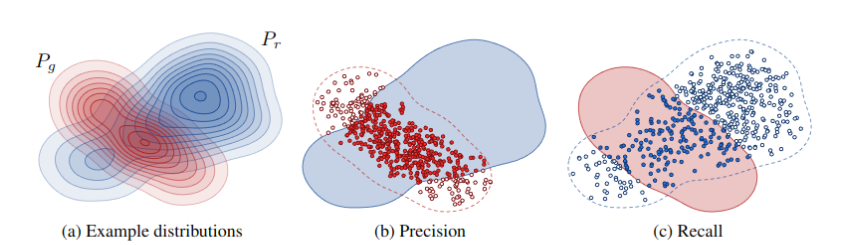
\includegraphics[width=\linewidth]{../images/2_PrecisionRecallManifold_si.png}
    %\label{fig:precision-recall-manifold}
    %\source{\cite{2ImprovedPrecisionRecall} Figure 1}
\end{figure}

Sebbene \textit{fidelity} e \textit{diversity} siano concetti centrali per la valutazione della qualità dei modelli generativi, risultano difficili da quantificare direttamente a causa della loro natura astratta.
Si riduce quindi il problema del calcolo della \textit{fidelity} e \textit{diversity} a quello della \textit{precision} e \textit{recall} (che offrono una formalizzazione più operativa di questi concetti, fornendo una base matematica per una valutazione quantitativa).\

Entrambe si basano sul concetto di \textbf{supporto} della distribuzione. Dato un numero limitato di campioni, definire un supporto continuo è un problema non banale. 
Molte delle metriche si preoccupano quindi di stimare il supporto e stabilire un criterio operativo per determinare la somiglianza tra due distribuzioni, il grado di sovrapposizione dei supporti stimati.
In questo contesto la stima del supporto è detta \textbf{manifold}.

\section{Improved Precision and Recall}
\label{sec:improved-precision-and-recall}

Nonostante il nome \textit{Improved Precision and Recall} possa suggerire un miglioramento rispetto a una versione precedente e meno sofisticata di \textit{precision and recall}, 
la metrica proposta da Tuomas Kynkäänniemi et al., 2019 \cite{2ImprovedPrecisionRecall}, precede temporalmente, in realtà, quella che sarà presentata successivamente, ovvero la metrica denominata più semplicemente \textit{Precision and Recall Coverage}. 
Di fatto, si tratta della forma più semplice di \textit{precision-recall} analizzata in questo lavoro, e rappresenta il punto di partenza per la nostra analisi.

Sia \(R\) il dataset di campioni reali (in genere dati usati per l'addestramento della rete) e \(G\) il dataset di campioni generati dalla rete neurale, identifichiamo con \boldsymbol{\Phi_R} e \boldsymbol{\Phi_G} (tendenzialmente con \boldsymbol{\Phi_R} = \boldsymbol{\Phi_G}) lo spazio delle caratteristiche e \(\Phi_R\) e \(\Phi_G\) i vettori di feature estratti da \(R\) e \(G\) rispettivamente.

È importante sottolineare che, come vedremo anche successivamente nella parte sperimentale, la scelta dell'estrattore di feature è cruciale per la corretta valutazione delle metriche di valutazione dei GAN.

Il manifold stimato a partire da \(R\) e \(G\) è un insieme di ipersfere, ciascuna con un raggio definito e centrate nei vari punti di \(\Phi_R\) e \(\Phi_G\). Il raggio di queste ipersfere è 
determinato da un iperparametro \texttt{k} che rappresenta il numero dei \textbf{nearest neighbors (NN)} da considerare. 

Possiamo quindi definire una funzione binaria che determini se un certo punto appartiene al manifold o meno:
\begin{equation}
    f_{ipr}(x, \Phi) = 
    \begin{cases}
        1 & \text{if }~~ \exists ~ y \in \Phi \text{ such that } ||x - y||_2 \leq ||y - NN_k(y, \Phi)||_2 \\
        0 & \text{otherwise.}
    \end{cases}
\end{equation}

Dove \(NN_k(y, \Phi)\) è il \texttt{k}-esimo vicino più prossimo di \texttt{y} in \(\Phi\).

La Precision e la Recall possono essere quindi definite come:
\begin{equation}
    Precision(\Phi_R, \Phi_G) = \frac{1}{|\Phi_G|} \sum_{g \in \Phi_G} f_{ipr}(g, \Phi_R)
\end{equation}
\begin{equation}
    Recall(\Phi_R, \Phi_G) = \frac{1}{|\Phi_R|} \sum_{r \in \Phi_R} f_{ipr}(r, \Phi_G)
\end{equation}

Nominalmente la Precision misura la percentuale di punti di \(\Phi_G\) che ricadono nel manifold di \(\Phi_R\) e la Recall la percentuale dei punti di \(\Phi_R\) che ricadono nel manifold di \(\Phi_G\).
Come tali le due metriche sono quindi normalizzate e assumono valori compresi tra \texttt{0} e \texttt{1}.
Come ripeteremo in seguito la metrica risulta dipendente dall'iperparametro \texttt{k} e in particolare pare che per \texttt{k = 3} si ottengano i risultati migliori.

\section{Density and Coverage}
\label{sec:density-and-coverage}

Come vedremo nel capitolo seguente l'\textit{Improved Precision Recall} soffre la presenza di \textit{outliers} nei datasets, vale a dire che il manifold stimato da \(R\) e \(G\) può essere fortemente influenzato da pochi punti molto distanti dalla distribuzione principale e quindi la presenza di molti dati generati in una zona vicina a questi outliers può portare a un errata alta stima della \textit{fidelity-precision}.
La \textit{Density and Coverage} è una metrica che cerca di mitigare questo problema (come analizzato da Muhammad Ferjad Naeem et al., 2019 \cite{3ReliableFidelityDiversityMetrics}). 

Invece che contare se le varie ipersfere in $\Phi_R$ contengono almeno un punto di $\Phi_G$, la \textit{Density} conta quanti punti di $\Phi_G$ sono inclusi in ciascuna ipersfera centrata su $\Phi_R$. Viene quindi scalato il risultato per il numero di ipersfere totali per il valore di \texttt{k} (si suppone che ciascuna ipersfera contenga almeno \texttt{k} punti).
Questo conporta però che la \textit{density} non è una metrica normalizzata e in certi casi assume valori maggiori di \texttt{1}. La formula è la seguente: 
\begin{equation}
    Density(\Phi_R, \Phi_G) = \frac{1}{k|\Phi_G|} \sum_{g \in \Phi_G} \sum_{r \in \Phi_R} \mathbbm{1}_{||r - g||_2 \leq ||g - NN_k(g, \Phi_G)||_2}
\end{equation}

Rispetto alle altre metriche in cui si poteva apprezzare la simmetria fra le formule per la stima di \textit{fidelity} e \textit{diversity}, in questo caso la \textit{Coverage} è una metrica completamente diversa dalla \textit{Density}. Questo perchè rispetto a $\Phi_G$, $\Phi_R$ non dovrebbe presentare \textit{outliers}.
La Coverage valuta se ogni dato reale \(r \in \Phi_R \)​ è rappresentato da almeno un punto generato \(g \in \Phi_G \)​, costruendo il manifold in \(\Phi_R\) e verificando se esiste almeno un punto di \(\Phi_G\) in ciascuna ipersfera. 

Anticipando la sezione che seguirà \textit{Precision Recall Curve}, è utile definire una funzione binaria che determini per la \textit{Coverage} se un certo punto appartiene a questa nuova definzione di manifold:
\begin{equation}
    f_{cov}(x, \Phi_x, \Phi_y) = 
    \begin{cases}
        1 & \text{if }~~ \exists ~ y \in \Phi_y \text{ such that } ||x - y||_2 \leq ||x - NN_k(x, \Phi_x)||_2 \\
        0 & \text{otherwise.}
    \end{cases}
\end{equation}

La formula della metrica sarà quindi:
\begin{equation}
    Coverage(\Phi_R, \Phi_G) = \frac{1}{|\Phi_R|} \sum_{r \in \Phi_R} f_{cov}(r, \Phi_R, \Phi_G)
\end{equation}

La formula potrebbe sembrare molto simile a quella dell'Improved Precision ma con un'importante differenza, ci chiediamo se esiste almeno un punto di $\Phi_G$ per ciascuna ipersfera costruita su $\Phi_R$ e non se per ciascun punto di $\Phi_G$ esiste una ipersfera che lo contiene. 

\begin{figure}[htbp]
    \centering
    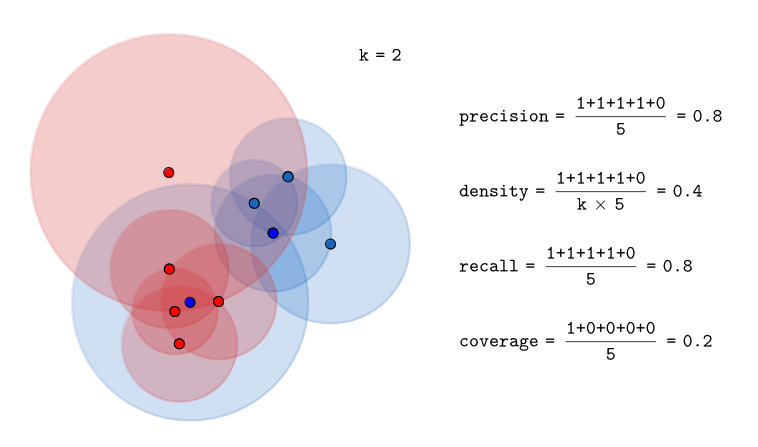
\includegraphics[width=\linewidth]{../images/prdc.png}
    %\label{fig:precision-recall-manifold}
    %\source{\cite{2ImprovedPrecisionRecall} Figure 1}
\end{figure}

Al contrario della Density, la Coverage è una metrica normalizzata e assume valori compresi tra 0 e 1.

Sperimentalmente, si è verificato che un valore di \texttt{k = 5} fornisce risultati ottimali, bilanciando la granularità delle ipersfere e la loro rappresentatività del manifold.

\section{Probabilistic Precision and Recall}  
\label{sec:probabilistic-precision-and-recall}

Un altro approccio al problema della stima del manifold consiste nel considerare la densità di probabilità delle distribuzioni reali e generate. Le formule utilizzate sono simili a quelle dell'\textit{Improved Precision e Recall},
ma con una differenza cruciale: invece di utilizzare una funzione di scoring binaria (\(f_{ipr}\)), si valuta la probabilità che un punto appartenga al manifold stimato. 
Questa probabilità viene calcolata dividendo il supporto in sottosupporti locali (\textit{subSupports}). 
Seguendo il lavoro di Dogyun Park et al., 2023 \cite{4ProbabilisticPrecisionRecall}, la probabilità di un punto \(x\) di appartenere a un sottosupporto centrato su \(y\) è definita come:
\begin{equation}
    P(x \in subSupp(y)) = 
    \begin{cases}
        1 - \frac{||x - y||_2}{\tau} & \text{se } ||x - y||_2 \leq \rho \\
        0 & \text{altrimenti.}
    \end{cases}
\end{equation}

La probabilità che un punto appartenga al manifold stimato viene quindi calcolata calcolando la probabilità che il dato non appartenga all'intersezione fra tutti i complementari dei sottosupporti locali
(supponendo quindi l'indipendenza degli eventi \(x \in subSupp^C(y)\) \(\forall y\)):
\begin{equation}
    P(x \in manifold(\Phi_y))) = 1 - \prod_{y \in \Phi_y} (1 - P(x \in subSupp(y)))
\end{equation}

Per la precision, la somma itera \(x\) su \(\Phi_G\) con manifold calcolato su \(\Phi_R\), mentre per la recall, si inverte il ruolo dei due dataset:
\begin{equation}
    Precision(\Phi_R, \Phi_G) = \frac{1}{|\Phi_G|} \sum_{g \in \Phi_G} P(g \in manifold(\Phi_R)),
\end{equation}
\begin{equation}
    Recall(\Phi_R, \Phi_G) = \frac{1}{|\Phi_R|} \sum_{r \in \Phi_R} P(r \in manifold(\Phi_G)).
\end{equation}

La variabile \(\rho\) gioca un ruolo cruciale in questo approccio, rappresentando il raggio delle ipersfere usate per stimare i sottosupporti locali. Per evitare sovrastime, si adotta una strategia simile alla \textit{Kernel Density Estimation} con varianza fissata, definendo \(\rho\) come segue:  
\begin{equation}
    \rho(\Phi) = \alpha \cdot \frac{1}{|\Phi|} \sum_{x \in \Phi} ||x - NN_k(x, \Phi)||_2
\end{equation}

dove \(\alpha\) è un nuovo iperparametro (con valore consigliato \(\alpha = 1.2\)). Per la precision si adotta quindi \(\rho(\Phi_R)\), mentre per la recall si utilizza \(\rho(\Phi_G)\).

L'approccio probabilistico è particolarmente utile perché affronta i limiti delle metriche basate sul \texttt{k}-Nearest Neighbor. La scelta di una \(\rho\) costante pari alla media delle distanze \(k\)-NN sopprime l’influenza degli outliers, riducendo la sovrastima del manifold in regioni scarsamente popolate 
e rende la metrica più robusta alla scelta di \texttt{k}, minimizzando la sensibilità della metrica ai cambiamenti del numero di vicini considerati.  

Sempre seguendo la letteratura il valore di \texttt{k} consigliato è \texttt{k = 4}.

\section{Precision and Recall Coverage}
\label{sec:precision-and-recall-coverage}

L'ultima metrica che verrà presentata è la \textit{Precision and Recall Coverage}, proposta da Fasil Cheema et al., 2023 \cite{1PrecisionRecallCover}.

Mantenendo la formalizzazione della sezione precedente si introduce un nuovo iperparametro \texttt{k' = Ck}. L'idea è quella di fornire un nuovo elemento per regolare la dimensione del manifold, e in particolare
le aree da considerare trascurabilmente piccole e quelle sufficientemente grandi. L'algoritmo proposto prevede per la Precision di costruire un manifold su \(\Phi_G\) con ipersfere con raggio pari alla distanza dal \texttt{k'}-th nearest neighbor
e contare il numero di ipersfere che contengono almeno \texttt{k} punti di \(\Phi_R\), si divide quindi per il numero di ipersfere totali (la dimensione di \(\Phi_G\)). 
Per la Recall si procede in modo analogo ma invertendo i ruoli di \(\Phi_R\) e \(\Phi_G\).

È importante notare come la metrica sia fondamentalmente la stessa della Coverage ma non è più sufficiente che esista un unico punto di \(\Phi_R\) in un ipersfera di \(\Phi_G\) ma è necessario invece che ce ne siano almeno \texttt{k}.
\begin{equation}
    Precision(\Phi_R, \Phi_G) = \frac{1}{|\Phi_G|} \sum_{g \in \Phi_G} \mathbbm{1}_{|\{ r \in \Phi_R, \text{s.t.} ||r - g||_2 \leq ||r - NN_{k'}(r, \Phi_R)||_2 \}| \geq k}
\end{equation}
\begin{equation}
    Recall(\Phi_R, \Phi_G) = \frac{1}{|\Phi_R|} \sum_{r \in \Phi_R} \mathbbm{1}_{|\{ g \in \Phi_G, \text{s.t.} ||g - r||_2 \leq ||g - NN_{k'}(g, \Phi_G)||_2 \}| \geq k}
\end{equation}

In questo caso l'aggiunta di un nuovo parametro, nonostante aumenti la complessità combinatoria di possibili valori assegnabili, si verifica sperimentalmente che mantenendo \texttt{C=3} la scelta di \texttt{k} e conseguentemente di \texttt{k'} può essere arbitraria
ottenendo comunque buoni risultati.

\section{Precision Recall Curve}  
\label{sec:precision-recall-curve}

Studi recenti \cite{5RevisitingPrecisionRecall, 6UnifyingPrecisionRecall, 7AssessingWithPrecisionRecall} hanno dimostrato che precision e recall possono essere interpretate come combinazioni lineari degli errori di tipo I e II di un classificatore binario ottimo.
Questa formulazione consente di costruire un limite superiore per la Precision e la Recall anche utilizzando un classificatore binario sub-ottimale. 
Inoltre, permette di analizzare il trade-off tra Precision e Recall tramite una curva, di cui le metriche viste in precedenza rappresentano solo i valori estremi.

I classificatori per la costruzione della curva Precision-Recall si basano sui manifold stimati. Le formule per i classificatori associati alle metriche sono:
\begin{equation}
    f_{\lambda}^{ipr}(x) = \mathbbm{1}_{\lambda \cdot |\{ r \in \Phi_R, \text{s.t.} ||r - x||_2 \leq ||r - NN_k(r, \Phi_R)||_2 \}| \geq |\{ g \in \Phi_G, \text{s.t.} ||g - x||_2 \leq ||g - NN_k(g, \Phi_G)||_2 \}|}
\end{equation}
\begin{equation}
    f_{\lambda}^{cov}(x) = \mathbbm{1}_{\lambda \cdot |\{ r \in \Phi_R, \text{s.t.} ||r - x||_2 \leq ||r - NN_k(x, \Phi_G)||_2 \}| \geq |\{ g \in \Phi_G, \text{s.t.} ||g - x||_2 \leq ||g - NN_k(x, \Phi_R)||_2 \}|}
\end{equation}

È interessante notare come le condizioni di appartenenza agli insiemi la cui cardinalità viene confrontata siano analoghe alle condizioni per \(f_{ipr}\) e \(f_{cov}\) con la differenza che qui andiamo a contare il numero di punti che soddisfano la condizione e non se esiste almeno un punto che la soddisfi.

La formula per \(f_{\lambda}^{ipr}\) può essere interpretata come una forma di Kernel Density Estimation (KDE) con bandwidth variabile.

\begin{equation}
    f_{\lambda}^{ipr}(x) = \mathbbm{1}_{\frac{\hat{p}(x)}{\hat{q}(x)} \geq \frac{1}{\lambda}},
\end{equation}

dove \(\hat{p}(x)\) e \(\hat{q}(x)\) rappresentano le densità stimate dai manifold reali e generati rispettivamente. In questa formulazione, il parametro \(\lambda\) agisce come un fattore di soglia che modula la decisione del classificatore:  

- \(\lambda \to 0\): Include quasi tutti i punti, abbassando la precisione e massimizzando la recall.  

- \(\lambda \to \infty\): Include solo i punti con densità generata molto bassa, massimizzando la precisione ma riducendo la recall.

Dal momento che questi classificatori vanno a cotruire un limite superiore, è possibile prendere il minimo fra le curve ottenute con i diversi classificatori per ottenere una stima più precisa.

\section{Altre metriche e funzioni correlate}
\label{sec:altre-metriche}

Per aggiungere un'appendice alla sezione precedente, sono state brevemente sfruttate altre metriche/classificatori accennati nel medesimi paper e in particolare nell'articolo di Benjamin Sykes et al, 2024 \cite{6UnifyingPrecisionRecall}. 
Tra questi risulta il knn classifier e il parzen classifier.
\begin{equation}
    f_{\lambda}^{knn}(x) = \mathbbm{1}_{\lambda |\{ r \in \Phi_R, \text{s.t.} ||r - x||_2 \leq ||r - NN_k(x, \Phi_U)||_2 \}| \geq |\{ g \in \Phi_G, \text{s.t.} ||g - x||_2 \leq ||g - NN_k(x, \Phi_U)||_2 \}|}
\end{equation}
\begin{equation}
    f_{\lambda}^{parzen}(x) = \mathbbm{1}_{\lambda |\{ r \in \Phi_R, \text{s.t.} ||r - x||_2 \leq \rho(\Phi_G) \}| \geq |\{ g \in \Phi_G, \text{s.t.} ||g - x||_2 \leq \rho(\Phi_R) \}|}
\end{equation}

con \(\Phi_U = \Phi_G \cup \Phi_R \) e \(\rho(\Phi)\) definito come nella sezione relativa a \textit{Probabilistic Precision and Recall} (\(\alpha = 1\)), vale a dire che il raggio delle ipersfere è fissato alla media delle distanze \texttt{k}-NN.

\(f_{\lambda}^{knn}\) è fondamentalmente analogo al \(f_{\lambda}^{cov}\) classifier ma costruisce l'ipersfera su entrambi i dataset.
Il \(f_{\lambda}^{parzen}\) classifier invece nutre delle somiglianze con il \(f_{\lambda}^{ipr}\) classifier ma costruisce l'ipersfera con un raggio fisso, è quindi per transitività simile ad una KDE con bandwidth costante.

Sebbene non sia propriamente una metrica di valutazione per i GAN, la Kernel Density Estimation è un metodo di stima della densità di probabilità di un dataset, ed è stata utilizzata nei nostri esperimenti per osservare alcune caratteristiche dei dataset reali e generati.
In particolare sono state sfruttate l'approssimazione di \textbf{Silverman} e nelle fasi di testing anche la stima di \textbf{Scott}.

La stima della densità tramite Kernel Density Estimation (KDE) con un kernel gaussiano può essere espressa come:
\begin{equation}
    \hat{f}(x) = \frac{1}{n h} \sum_{i=1}^{n} K\left(\frac{x - x_i}{h}\right)
\end{equation}

dove \(K(x)\) è, nel nostro caso, il kernel gaussiano definito come:
\begin{equation}
    K(x) = \frac{1}{\sqrt{2\pi}} \exp\left(-\frac{x^2}{2}\right)
\end{equation}

\(h\) è il parametro di bandwidth e \(n\) rappresenta il numero di punti nel datases.
\begin{equation}
    h_{\text{Scott}} = n^{-\frac{1}{d+4}} \cdot \sigma
\end{equation}
\begin{equation}
    h_{\text{Silverman}} = \left(\frac{4}{3n}\right)^{\frac{1}{5}} \cdot \sigma
\end{equation}

dove \(\sigma\) è la deviazione standard del dataset e \(d\) è la dimensione dei dati.

Un ultima funzione che è stata utilizzata per valutare la qualità dei singoli dati è il \textbf{realism score} proposto da \cite{2ImprovedPrecisionRecall} e definito come:
\begin{equation}
    \text{realism score}(g) = \max_{r \in \Phi_R} \{ \frac{||r-NN_k(r)||_2}{||g-r||_2} \}
\end{equation}

Un punto che ha realism score \(\ge 1\) è molto simile ai dati reali, viceversa un punto con realism score in [0,1) è molto diverso dai dati reali.

Per quanto riguarda l'applicazione dei classificatori per la costruzione della Precision Recall Curve, i dataset sono stati divisi in training e testing set con split specificati nella parte sperimentale. Mentre per gli estrattori di caratteristiche sono state utilizzate metriche \textbf{informate} e \textbf{non informate} del dominio dei dati (per queste chiariremo meglio in seguito).

\chapter{Esperimenti}\label{ch:chapter2}

Per la valutazione delle metriche sono stati condotti diversi esperimenti che possono essere suddivisi in due macro-categorie dipendentemente dal tipo di dataset utilizzato:
\begin{itemize}
    \item \textbf{Toy Dataset}: dataset generati artificialmente per testare il comportamento delle metriche in condizioni controllate.
    \item \textbf{Real World Dataset}: dataset reali per testare il comportamento delle metriche in condizioni reali.
\end{itemize}
Le sezioni seguenti descrivono come sono state implementate le metriche, gli esperimenti così come le distribuzioni di dati utilizzate.\
La ragione per cui sono stati condotti esperimenti su dateset generati artificilmente (ovvero di matrice matematica, non derivanti dalla realtà o generati da reti neurali) è che in questo modo è stato possibile osservare il comportamento delle metriche in condizioni controllate, ideali e per poter confrontare i risultati ottenuti con quelli attesi presenti nella letteratura.\
Fanno infatti parte dei test su 'toy dataset', i test di corretta implementazione ovvero un'analisi comparativa delle diverse implementazioni in codice delle metriche. Tali test hanno il fine di verificare che le metriche restituiscano valori corretti validando gli altri esperimenti.\

I dataset reali sono stati utilizzati per testare il comportamento delle metriche in condizioni reali, ovvero per verificare se le metriche si comportano come ci si aspetta in situazioni non ben definite, con distribuzioni di dati non note, ben distanti da quelle ideali. Questo infatti, come vedremo, può sollevare criticità, ad esempio dovute alla assenza di certe categorie di dati o alla presenza di dati non ben distribuiti.\
Un altro elemento dei dataset reali è che spesso questi non sono di carattere prettamente numerico, nei dataset analizzati ad esempio, abbiamo immagini di farfalle e partiture musicali. Questo comporta la necessità di trasformare i dati per poterli utilizzare, e il processo di \textbf{estrazioni di caratteristiche} può equivalere ad una perdita di dati significativi o, al contrario, ad una sovrabbondanza di dati non significativi.\

\section{Toy Dataset}
\label{sec:toy-dataset}

Come anticipato nell’introduzione di questo capitolo, i Toy Dataset sono dataset generati artificialmente tramite funzioni matematiche che producono dati in modo casuale ma controllato. Per questi esperimenti, sono state utilizzate principalmente due tipi di distribuzioni di dati numerici con dimensione variabile: la distribuzione uniforme e la distribuzione normale. In una specifica categoria di esperimenti, sono stati aggiunti anche outliers, ossia dati che si discostano significativamente dalla distribuzione principale, con l'obiettivo di valutare la robustezza delle metriche in presenza di anomalie.

Gli esperimenti condotti si ispirano a quelli presenti in letteratura e hanno diversi obiettivi, tra cui:
\begin{itemize}
    \item Testare l'influenza degli iperparametri delle metriche sul loro comportamento.
    \item Valutare la risposta delle metriche alla presenza di outliers.
    \item Studiare l'impatto della dimensione del dataset sui risultati.
    \item Confrontare le implementazioni delle metriche esistenti comparando numericamente i risultati su dataset identici e confrontando i grafici delle pr-curve con quelli presenti in letteratura.
\end{itemize}

Per ciascun esperimento sono stati prodotti grafici che illustrano i risultati ottenuti. L'unica eccezione è rappresentata dai test di corretta implementazione delle metriche, dove la validazione è stata condotta principalmente tramite confronti numerici. La scelta delle tipologie di grafici è stata guidata dall'obiettivo di facilitare il confronto con i risultati riportati in letteratura quindi in certe circostanza anche a discapito della chiarezza dei grafici stessi.

Data la complessità computazionale di alcuni esperimenti, i risultati intermedi e finali sono stati salvati in file \texttt{.npy}, permettendo analisi approfondite e riproducibilità senza dover ripetere calcoli onerosi. Questo approccio non solo consente una gestione efficiente dei dati, ma permette anche un'analisi successiva più flessibile, ad esempio per esplorare ulteriori correlazioni, per verificare ipotesi aggiuntive o per produrre grafici alternativi.

\subsection{Parametro k e dimensione del dataset}
\label{subsec:k-dataset-dimension}

Come abbiamo visto, tutte le metriche analizzate si basano sulla distanza dei dati rispetto ai loro vicini. Uno dei parametri più determinanti è l'ordine \texttt{k} del vicino più prossimo. Secondo la letteratura, i valori ottimali di \texttt{k} variano in base alla metrica analizzata: per l’\textbf{improved precision recall} \texttt{k = 3}, per la \textbf{probabilistic precision recall} \texttt{k = 4}, per la \textbf{precision recall coverage} \texttt{k=\(\sqrt{|\Phi|}\)} indicando con \(|\Phi|\) la dimensione del dataset reale e/o generato (o \texttt{k = 3} se \texttt{C = 3})
, mentre per \textbf{density} e \textbf{coverage} \texttt{k = 5}. Questi valori riflettono un compromesso ottimale tra stabilità della metrica e sensibilità alla densità locale. Ci si aspetta che l'aumento della dimensione del dataset porti a un incremento dei valori delle metriche, poiché una maggiore quantità di dati aumenta la densità dei punti, migliorando la rappresentatività delle distribuzioni e riducendo l’effetto del rumore.

L'analisi è stata condotta su dataset generati una sola volta, mantenuti costanti e identici per la valutazione di tutte le metriche, questo per garantire coerenza nei risultati. Sono state utilizzate, come anticipato precedentemente, due diverse distribuzioni: uniforme e normale. I test sono stati effettuati per valori di \texttt{k} variabili da 1 a 10 vale a dire \([1,2,3,\dots,8,9,10]\) e per dimensioni del dataset crescenti esponenzialmente, da 500 a 16000 punti (\([500,1000,2000,4000,8000,16000]\)). Ogni dato è rappresentato come un vettore in \(\mathbb{R}^{64}\).

Per presentare i risultati, sono state utilizzate delle \textbf{heatmap}, che mostrano i valori delle metriche in funzione di \texttt{k} e della dimensione del dataset. In queste rappresentazioni, il rosso indica valori prossimi a \texttt{1.}, mentre il verde valori vicini a \texttt{0.}. Sebbene le heatmap non offrano precisione numerica immediata, forniscono una visione d’insieme sulle tendenze generali delle metriche e facilitano il confronto con gli esperimenti presenti in letteratura \cite{3ReliableFidelityDiversityMetrics}. Nel paper di riferimento, sono state prodotte heatmap solo per le metriche di \textbf{improved precision recall} e \textbf{density and coverage} e con distribuzioni normali identiche, ma per completezza sono state prodotte anche per le altre metriche presentate nel capitolo precedente e per distribuzioni uniformi, per evidenziare eventuali comportamenti che si possono presentare in situazioni diverse.

\subsection{Dimensione del dataset e dimensione dei dati}
\label{subsec:dataset-data-dimension}

In questo caso, l'analisi condotta non ha un riscontro diretto nella letteratura esistente, ovvero non presenta antecedenti (quantomeno per gli articoli presi in analisi). L'obiettivo è determinare come la \textbf{dimensione del dataset} possa influenzare la densità dei dati della distribuzione (a dimensione dei dati fissata) e, conseguentemente, il valore delle metriche. I risultati di questa analisi costituiscono una parte fondamentale per le analisi su dati reali, dove la scelta del numero di caratteristiche da considerare può risultare determinante.

In questo esperimento, abbiamo considerato una distribuzione normale (\(\mathcal{N}(0, I)\)) dei dati con \textbf{dimensione del dataset variabile} da 50 a 1600, con valori \([50, 100, 200, 400, 800, 1600]\), e \textbf{dimensione dei dati} da 2 a 64, con valori \([2, 4, 8, 16, 32, 64]\). 
A differenza degli esperimenti precedenti, rappresentati tramite heatmap, qui l'assenza di un riscontro nella letteratura ci ha permesso di utilizzare \textbf{grafici a linee bidimensionali} per rappresentare i risultati (data la ridotta dimensionalità, almeno per le dimensioni di interesse, di uno degli iperparametri da regolare, ovvero la dimensione dei dati).
Il valore dell'\textbf{iperparametro \( k \)} è stato scelto in accordo con quanto suggerito nei vari articoli, per garantire la massima efficacia della metrica. Le misurazioni sono state ripetute 25 volte e successivamente mediate. Anche in questo caso, il calcolo è stato effettuato in parallelo.

\subsection{Outliers}
\label{subsec:outliers}

Una delle proprietà più rilevanti da esaminare nelle diverse metriche è la loro resistenza agli outliers. In linea con la letteratura, abbiamo analizzato come i valori delle metriche cambiano in presenza di dataset con distribuzione normale, \textbf{senza outliers} e con \textbf{outliers} inseriti sia nei dati reali sia in quelli generati.

L’esperimento si è svolto considerando una distribuzione reale fissa \( X \sim \mathcal{N}(0, I) \) e una distribuzione generata \( Y \sim \mathcal{N}(\mu, I) \), con uno shift della media \(\mu\) variabile in \([-1,1]\) (con \textbf{step} di \texttt{0.05}). In aggiunta, sono stati esaminati due scenari di outliers, in cui un campione estremo a \( x = +1 \) è stato aggiunto ai dati reali o a quelli generati. 
Lo spazio di lavoro è stato definito in \( \mathbb{R}^{64} \), con vettori reali centrati sull’origine e campioni generati con media variabile lungo la direzione del vettore unitario.
Data l'onerosità computazionale di questo esperimento, sono stati considerati dataset con 1000 punti per ciascuna distribuzione senza mediazione. I calcoli sono stati effettuati in parallelo per ridurre i tempi di esecuzione.

Oltre alle metriche di \textbf{precision-recall} e \textbf{density-coverage} (come nel paper), i test sono stati condotti anche sulle metriche di \textbf{probabilistic precision-recall} e \textbf{improved precision-recall}. Per ciascuna metrica sono stati utilizzati i valori degli iperparametri suggeriti dai rispettivi articoli.

In assenza di outliers, ci si attende che i valori delle metriche diminuiscano gradualmente man mano che \(\mu\) si allontana da zero, indicando correttamente la divergenza tra le due distribuzioni. Ci aspettiamo quindi, anche che per \(\mu = 0\) si abbia un massimo assoluto molto vicino a \texttt{1.} (data la completa sovrapposizione delle due distribuzioni).\

\subsection{Comparazione con implementazioni esistenti}
\label{subsec:comparazione}

Non tutti i papers analizzati presentavano un'implementazione delle metriche in codice. Sono stati svolti dei test confrontando su dataset identici le diverse implementazioni delle metriche presenti in letteratura \cite{2ImprovedPrecisionRecall} \cite{3ReliableFidelityDiversityMetrics} \cite{4ProbabilisticPrecisionRecall}.
Non sono stati possibili confronti diretti per quanto riguarda la \textbf{precision-recall coverage}, in quanto non sono state trovate implementazioni in codice, mentre per la \textbf{improved precision-recall} sono state confrontate due diverse implementazioni.

Sono state scelte tre diverse distribuzioni di dati: distribuzione uniforme, distribuzione normale e distribuzione normale con media in \(3/\sqrt{dim}\). Ciascuna distribuzione è stata generata con dimensione del dataset pari a 10000 e dimensione dei dati pari a 64.\
I risultati sono stati riportati su un file \texttt{log.txt} per poter essere confrontati in un secondo momento.\
Allo scopo di velocizzare la computazione e ridurre il tempo di esecuzione, i test comparativi per la \textbf{probabilistic precision-recall} e la \textbf{density-coverage} sono stati eseguiti con ordine \( k = 3 \), nonostante i valori ottimali suggeriti dalla letteratura siano diversi. Questo hai infatti permesso di calcolare le distanze intraset una sola volta, evitando di ripeterle per ogni valore di \( k \) considerato che non eravamo interessati a valutare l'efficacia delle metriche quanto a confrontare le diverse implementazioni.

\subsection{Riproduzione delle pr-curve}
\label{subsec:pr-curve}

Anche per la riproduzione delle pr-curve sono stati utilizzati dataset generati artificialmente. L'articolo di riferimento per questo esperimento \cite{6UnifyingPrecisionRecall}, non presentava un'implementazione in codice delle metriche, ma solo i risultati ottenuti.\
Abbiamo quindi replicato le pr-curve per i quattro classificatori presentati nel paper, vale a dire il classificatore \textbf{ipr}, \textbf{coverage}, \textbf{knn} e \textbf{parzen}, per due differenti distribuzioni di dati, in particolare distribuzioni normali con media in \(0\) per i dati reali  e \(1/\sqrt{dim}\) e \(3/\sqrt{dim}\) per i dati generati (\(dim = 64\)).\ 

I classificatori hanno operato su un dataset di 20000 elementi, con 10000 elementi per ciascuna classe. 
Sono stati condotti gli esperimenti sia operando uno split dei dati dividendoli in training e test set al 50\% (ovvero 5000 punti effettivi per classe scelti casualmente sui 10000) sia senza split, ovvero costruendo il training set con tutti i dati reali e generati.\
Sono stati inoltre scelti due valori di \( k \) ovvero \(k = 4\) e \(k = \sqrt{n}\) (dove \(n\) è il numero di punti nel training set ed ha quindi cardinalità pari \(|\Phi|\) se si sta operando senza split o \(n = |\Phi|/2 \) se con split).\

Osservando i risultati del paper ci si aspetta che delle quattro pr-curve generate, la coverage-curve sia la più estrema, ovvero quella che produce un risultato migliore (più vicino al classificatore ottimale).\
Un'altra proprietà attesa è la simmetria delle curve rispetto alla diagonale, questo è dovuto al tipo di distribuzione dei dati utilizzata, al fatto che i training set fossero bilanciati e le metriche simmetriche a loro volta.\
Dei test preliminari hanno poi mostrato fondamentale la scelta del range di valori e degli step per quanto riguarda la variabile \( \lambda \) (ovvero il parametro che regola la trade-off tra precision e recall). 
Come consigliato da \cite{7AssessingWithPrecisionRecall}, il range di valori è stato generato dalla formula \( \tan(\pi/2 * i/(g+1)) \) con \( i \in [1, g] \) e \( g = 1001\) il numero di valori generati. Questa trasformazione consente di esplorare diverse scale di \(\lambda\) con una densità variabile: i valori crescono rapidamente da 0 a 1, variano lentamente fino a \(\pi/2\)​, e infine aumentano rapidamente verso l'infinito. Questa caratteristica rende la funzione adatta per analizzare con precisione le transizioni critiche della PR-curve in regioni chiave, bilanciando una copertura fine e una rapida esplorazione delle estremità. 
In fase sperimentale sono state utilizzate altre funzioni per coprire il range di valori di \(\lambda\), ma la funzione sopra descritta è risultata la più adatta per l'analisi delle curve, e quella che ha prodotto i risultati più simili a quelli presenti in letteratura, pertanto l'unica di cui si riportano i risultati.

\section{Real World Dataset}
\label{sec:real-world-dataset}

Come anticipato nell'introduzione di questo capitolo, oltre agli esperimenti condotti in ambienti controllati, 
regolati e basati su dati sintetici, è fondamentale analizzare il comportamento delle metriche in condizioni reali, 
ovvero su dataset rappresentativi di problemi pratici. Questa fase di sperimentazione consente di testare l'applicabilità 
delle metriche in contesti che vanno oltre l’ambito strettamente numerico e teorico, avvicinandosi alle condizioni operative 
in cui tali strumenti dovrebbero operare. In particolare, l’obiettivo finale delle metriche studiate è proprio quello 
di fornire un supporto concreto nell’analisi della qualità dei dati generati, facilitando l’integrazione delle reti generative in applicazioni pratiche.

Gli esperimenti sui dati reali sono stati condotti su due dataset distinti: un set di immagini raffiguranti farfalle 
e una collezione di partiture musicali di Alessandro Scarlatti, compositore rappresentativo della musica barocca. 
Questi dataset presentano specificità intrinseche che richiedono l’estrazione di caratteristiche rilevanti dal dominio dei dati (in particolare per le immagini utilizzare i \texttt{raw data} sarebbe improponibile data la loro dimensione). 
Per le immagini delle farfalle si è scelto di lavorare con feature basilari, come istogrammi di colore e saturazione, per valutare l’abilità delle metriche nel rilevare differenze qualitative senza fare ricorso a rappresentazioni complesse o specifiche del dominio.
Nel caso delle partiture musicali, invece, le caratteristiche estratte sono state più mirate e informate dal dominio della musica barocca seguendo quanto descritto nella letteratura \cite{8OnTheEvaluationOfGenerativeModelsInMusic}. 
Sono state utilizzate, ad esempio, informazioni di carattere ritmico e tonali. Questo approccio permette di valutare le metriche su dati complessi con maggiore precisione.

Un ulteriore strumento di analisi utilizzato in questo contesto è la \textbf{Kernel Density Estimation} (\textbf{KDE}), che si è dimostrata particolarmente utile per ottenere una stima non parametrica della distribuzione dei dati. 
La \textbf{KDE} permette di visualizzare come i dati siano distribuiti nel loro spazio delle caratteristiche, fornendo così un quadro più completo delle relazioni tra i campioni reali e quelli generati. 
Questa informazione è cruciale per interpretare meglio il comportamento delle \textbf{metriche}, soprattutto quando si cerca di identificare regioni di alta o bassa densità che potrebbero indicare rispettivamente dati generati di alta qualità o outlier.

Infine, un obiettivo centrale di questa fase sperimentale è quello di verificare l'efficacia delle metriche nel discriminare dati generati di alta qualità da dati generati di bassa qualità, 
fungendo così da filtro ultimo per le reti generative. In questa ottica, le metriche potrebbero operare come strumento di selezione, scartando i dati che non soddisfano determinati standard di qualità e potenzialmente indicando i campioni da rigenerare.

\subsection{Butterflies}
\label{subsec:butterflies}

Il dataset di immagini di farfalle è stato utilizzato per valutare l’efficacia delle metriche in un contesto caratterizzato dall’uso di feature elementari, estratte senza ricorrere a una conoscenza specifica del dominio dei dati. 
A differenza del dataset di partiture musicali, qui si è scelto di non considerare caratteristiche strutturali o semantiche delle immagini, concentrandosi invece su proprietà visive di base quali le proprietà cromatiche e di intensità. 
Queste sono particolarmente semplici da estrarre in quanto basta calcolare gli istogrammi di colore, saturazione e valore, con il vantaggio che si può regolare la dimensione dello spazio delle caratteristiche, ad esempio scegliendo di lavorare con istogrammi ad un numero ridotto di bin.

Per ogni immagine sono stati calcolati sei tipi di istogrammi, utilizzati come feature per le metriche:
\begin{itemize}
    \item \textbf{Hue hitogram}: rappresenta la distribuzione delle tonalità di colore.
    \item \textbf{Saturation histogram}: descrive l'intensità cromatica dell'immagine.
    \item \textbf{Value histogram}: misura la luminosità, derivata dalla rappresentazione HSV.
    \item \textbf{Grayscale histogram}: calcolato come combinazione lineare dei valori RGB, distinto dal value histogram.
    \item \textbf{RGB histogram}: include le distribuzioni di colore separate per i canali rosso, verde e blu.
    \item \textbf{HSV histogram}: include tonalità, saturazione e valore in una rappresentazione unificata.
\end{itemize}
Gli istogrammi sono stati costruiti suddividendo il range di ciascuna caratteristica in 64 intervalli uniformi, detti "bin". Ogni bin rappresenta un intervallo specifico del valore della caratteristica e conta il numero di pixel dell'immagine che rientrano in quel range. La scelta di lavorare con 64 bin è stata motivata dalla necessità di mantenere un equilibrio tra la complessità delle feature e la capacità delle metriche di discriminare tra dati reali e generati (una maggiore quantità di informazioni potrebbe rendere più evidenti le differenze tra le distribuzioni).
Per gli istogrammi con più canali, vale a dire RGB e HSV, sono stati considerati 64 bin complessivi, ovvero 21 bin per ciascun canale. Questa scelta è stata fatta per mantenere la stessa dimensione dello spazio delle caratteristiche per tutti gli istogrammi, facilitando il confronto tra le diverse feature. È molto probabile infatti (e motivo di indagine degli esperimenti introdotti precedentemente sui toydataset) che la dimensione dei dati possa influenzare il valore delle metriche.

La distanza tra gli istogrammi è stata misurata utilizzando la norma \(l_1\)​ (distanza di \textbf{Manhattan} o \textbf{cityblock}) anziché la norma \(l_2\)​ (distanza euclidea). La norma \(l_1\)​ è risultata più adeguata in questo contesto, poiché, lavorando su distribuzioni discrete come gli istogrammi, consente di misurare l'area condivisa fra gli istogrammi piuttosto che la distanza tra i loro picchi che è di minor interesse in questo contesto.

Il rilevamento dei falsi positivi è stato effettuato utilizzando un classificatore \texttt{k}-NN, configurato con ​\(k=\sqrt{n/2}\), dove \(n\) è il numero di punti nel training set. In questo contesto, i falsi positivi sono definiti come dati generati che si collocano al di fuori del manifold dei dati reali, mentre i veri positivi rappresentano i dati generati che rientrano in tale manifold. L’approccio è analogo a quello adottato negli esperimenti sulle IPR-curve, ma senza variare il parametro \(\lambda\). 
Questo approccio eredita tutti i difetti della metrica improved precision recall, in particolare la sensibilità alla presenza di outliers. Tuttavia la sua semplicità offre un'opportunità rapida di verificare i limiti e le potenzialità del metodo di discriminazione di dati di alta e bassa qualità che verrà poi applicato con maggior rigore per i dati musicali.
L'immagine generata valutata dal classificare è stata di volta in volta rimossa dallo stimatore del manifold, in questo modo si è potuto identificare quei dati che risultassero degli outliers per la propria distribuzione.

Il dataset di farfalle usato per l'allenamento della rete generativa e quindi comprendente i dati reali è composto da 1000 immagini, mentre il dataset generato da 895 immagini. Data la natura delle metriche utilizzate (alcune di esse richiedevano che la dimensione dei due dataset fosse uguale) è stato impiegato per la valutazione la dimensione minima fra le due dimensioni dei dataset considerati, ovvero 895 immagini (per dataset).\
Nonostante la qualità variabile delle immagini reali (alcune delle quali contenevano artefatti o impurità), non sono state effettuate operazioni di pulizia. L’obiettivo era infatti verificare l’efficacia delle metriche indipendentemente dalla qualità dei dati.

In questo caso l'applicazione della KDE per le distanze inter e intra set è stata fondamentale per la comprensione dei risultati ottenuti, in quanto ha permesso di visualizzare le distribuzioni dei dati in uno spazio a dimensione ridotta, fornendo un quadro chiaro delle relazioni tra i campioni reali e quelli generati.\

\subsection{Scarlatti}
\label{subsec:scarlatti}

Al contrario del dataset di farfalle, per il dataset di partiture musicali è stato adottato un approccio più mirato e informato dal dominio dei dati. Per l'estrazione delle caratteristiche infatti sono state utilizzate informazioni di carattere ritmico e tonale, seguendo quanto descritto nella letteratura \cite{8OnTheEvaluationOfGenerativeModelsInMusic}.\

\begin{figure}[h]
    \centering
    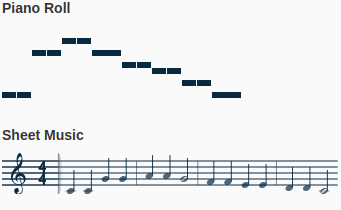
\includegraphics[width=0.5\textwidth]{../images/piano_roll.png}
    \caption{Esempio di rappresentazione di una partitura musicale in piano-roll}
\end{figure}

Il paper indicato, in particolare, presentava un implementazione delle metriche per l'estrazione di caratteristiche musicali basato su una rappresentazione delle partiture musicali in forma di \textbf{piano-roll}.
Il piano-roll è una rappresentazione grafica delle note musicali in cui l'asse delle ascisse rappresenta il tempo e l'asse delle ordinate rappresenta le note. Ogni cella della matrice corrisponde a una nota suonata in un determinato istante di tempo. Presenta tuttavia delle limitazioni, in quanto in condizioni particolari può esserci perdita di informazione.\
Invece che utilizzare il piano-roll, sono state estratte le caratteristiche direttamente dai file MIDI, quindi da una lista di note (\textbf{tuple}) con informazioni sul tempo, altezza, durata e strumento adoperato (nel nostro caso sempre e solo il clavicembalo), reimplementando le metriche del paper ma con questa diversa rappresentazione.\
Le caratteristiche estratte si dividono in due categorie: \textbf{caratteristiche ritmiche} e \textbf{caratteristiche tonali}. Le prime includono informazioni sul tempo e sulla durata delle note, mentre le seconde riguardano la tonalità delle note e le relazioni armoniche tra di esse.\
Tra le diverse distanze sono poi presenti: distanze scalari, distanze vettoriali e distanze matriciali.\

Le caratteristiche tonali considerate sono:
\begin{itemize}
    \item \textbf{number of pitches per measure} - il numero di toni diversi presenti in una singola battuta (vettore di dimensione 8)
    \item \textbf{pitch class histogram} - l'istogramma delle classi di toni presenti in una singola battuta (vettore di dimensione 12)
    \item \textbf{pitch class histogram per measure} - l'istogramma delle classi di toni presenti in una singola battuta (vettore di dimensione 12x8 = 96)
    \item \textbf{pitch class transition matrix} - la matrice di transizione delle classi di toni (matrice 12x12=144)
    \item \textbf{pitch range} - la differenza tra il tono più alto e il tono più basso (scalare)
    \item \textbf{average pitch shift} - la media delle variazioni di tono tra note consecutive (scalare)
\end{itemize}

Caratteristiche ritmiche:
\begin{itemize}
    \item \textbf{number of notes per measure} - il numero di note presenti in una singola battuta (vettore di dimensione 8)
    \item \textbf{note length histogram} - l'istogramma delle durata delle note presenti in una singola battuta (vettore di dimensione 24)
    \item \textbf{note length histogram per measure} - l'istogramma delle durata delle note presenti in una singola battuta (vettore di dimensione 24x8 = 192)
    \item \textbf{note length transition matrix} - la matrice di transizione delle durate delle note (matrice 24x24=576)
    \item \textbf{average IOI} - l'intervallo inter-onset medio, ovvero la media delle variazioni di durate di note consecutive (scalare)
\end{itemize}

Mentre per le immagini di farfalle avevamo un unico modello generativo per la generazione dei dati, per le partiture musicali sono stati utilizzati più modelli generativi, o meglio cinque versioni di uno stesso modello a diverse epoche di  \textit{training}.\

Il primo test eseguito è stato un \textbf{sanity check}, un controllo preliminare per garantire che le caratteristiche estratte mostrassero distribuzioni stabili e coerenti sui dati reali. 
Per fare ciò, sono state calcolate le KDE sulle distanze intra-set dei dati reali, suddivisi in \textbf{training} e \textbf{test} più \textbf{validation} set. Poiché entrambi i set contengono dati reali, una divergenza tra le distribuzioni, o una difficoltà
ad individuare una \textbf{bandwidth}, indicherebbe un problema nell’approccio o nelle caratteristiche selezionate.

Sono stati quindi riprodotti gli esperimenti condotti sul dataset di farfalle, studiando le distribuzioni delle distanze intra-set per ciascuna caratteristica sempre tramite KDE. Avendo a disposizione più modelli generativi sono stati prodotti grafici a violino (\textbf{violin plots}) che accostano le due distribuzioni e permettono di stabilire rapidamente quale epoca di training abbia prodotto i dati più simili a quelli reali.\
Per validare ulteriormente i risultati ottenuti, sono state tracciate le pr-curve (che seppur basate sulle distanze fra i dati, operano direttamente nello spazio dei dati e non sulle distanze).\

Sempre come nei test sul dataset di farfalle, sono stati identificati i falsi positivi individuando i dati generati che non rientravano nel manifold dei dati reali. In questa fase sono state anche calcolate le overlaped area tra le KDE dei dati reali e i dati genati dalle diverse epoche. 
Questo ha permesso di stabilire numericamente per ciascuna metrica quale epoca di training avesse prodotto i dati più simili a quelli reali per numero di falsi positivi e per overlaped area.\ 

Con 'measure' si intende una singola battuta di musica, ovvero un'unità di tempo musicale, ad esempio se il tempo è 4/4, una battuta è composta da 4 semiminime (o 8 crome, o 16 semicrome, ecc.).\
La maggior parte dei dati musicali di musica barocca è scritta in 4/4 con 8 battute, per quei dati in cui il tempo non era specificato è stato considerato 4/4, e in caso di battute mancanti sono state aggiunte battute vuote.\
Sebbene si sia cercato di eliminare i dati mal generati, alcuni di essi sono stati comunque inclusi nel dataset con le considerazioni sopra descritte. Ci aspettiamo che questo possa influenzare i risultati delle metriche, in particolare vogliamo verificare che l'applicazione delle metriche come filtro, siano in grado di discriminare tali dati di bassa qualità.\
Delle 1000 partiture musicali per modello disponibili ne sono state scartate le prime 50 e le ultime 50, per un totale di 900 partiture musicali per modello.\
Gli altri iperparametri e distanze utilizzate sono state le stesse di quelle impiegate per il dataset di farfalle, fatta eccezione del valore di \texttt{k} che è stato impostato a \texttt{k = 3} per tutte le metriche. La motivazione è che ci aspettiamo che i dati musicali siano più fitti di quelli delle immagini (sopratutto date le caratteristiche estratte) e quindi un valore di \texttt{k} più basso dovrebbe permettere una stima del manifold più accurata.\

Infine, sempre per studiare le capacità delle metriche di discriminare dati di alta e bassa qualità, è stato adottato un approccio \textbf{leave-one-out} applicato però alla stima della KDE.\
È stato rimosso dalla KDE stimata dalle distanze inter-set fra dati reali e dati generati da una certa epoca, i contributi di ciascun dato generato e verificato se la \textbf{likelihood} di tale dato fosse inferiore ad un certo \textbf{threshold}.
Nel caso in cui la likelihood fosse inferiore al threshold il dato generato è da considerare un falso positivo.\
Come trashold è stato preso lo \texttt{0.05} percentile delle likelihood stimate con la KDE.\
Questo metodo, sebbene efficace, ha un enorme limitazione, infatti prendendo un percentile fisso avremo lo stesso numero di falsi positivi per ogni epoca di training, questo non ci permette di confrontare le epoche tra di loro, ma solo di valutare la capacità delle metriche di discriminare dati di alta e bassa qualità.\
Metodi più sofisticati prevedono di calcolare la GPD (Generalized Pareto Distribution) sulle likelihood stimate e prendere il threshold in modo da identificare con maggiore accuratezza l'insieme completo degli outliers, vedi \cite{9LeaveOneOut}, ma questo è stato considerato fuori dallo scopo di questo lavoro.
\chapter{Conclusioni}\label{ch:conclusioni}

\section{Risultati degli esperimenti sui toy-dataset}

\subsection{Parametro k e dimensione del dataset}
\label{sec:res-k-dataset-dim}

I primi esperimenti che abbiamo proposto nel capitolo precedente \ref{sec:toy-dataset} erano quelli relativi al robustezza delle metriche alla variazione degli iperparamentri quali \texttt{k} e la dimensione del dataset \(|\Phi|\).
In particolare ci siamo posti come obiettivo di riprodurre le heatmap presenti in \cite{3ReliableFidelityDiversityMetrics} per il confronto delle metriche di precisione-recall e density-coverage con distribuzioni normali per i dataset, ed estenderli a distribuzioni uniformi e alle metriche non analizzate dal paper.

\begin{figure}[!ht]
    \centering
    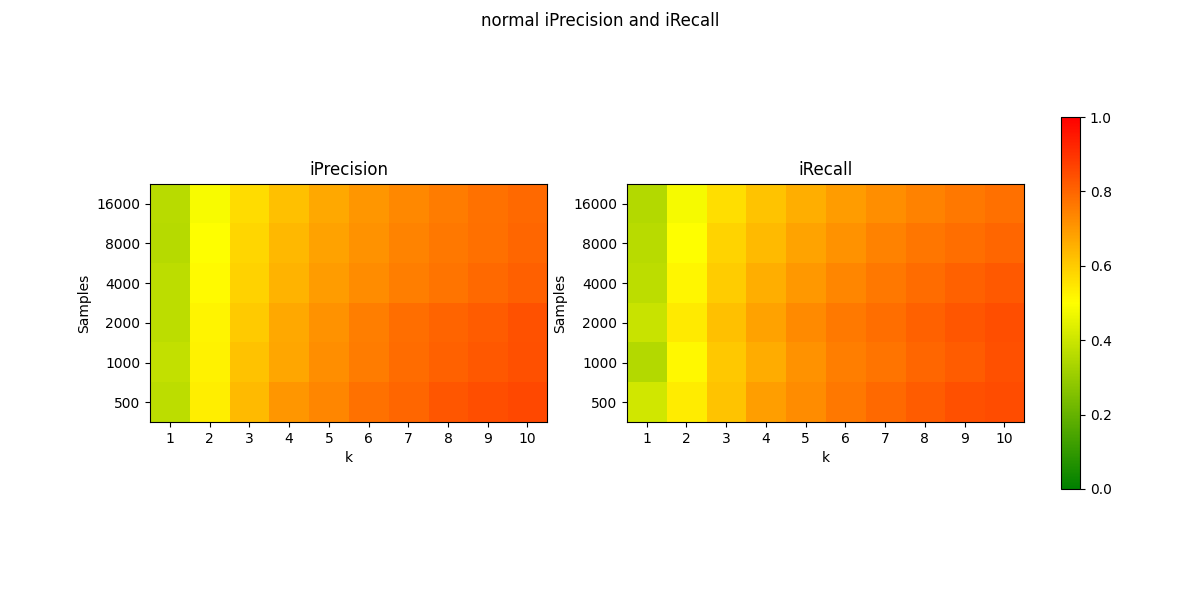
\includegraphics[width=0.8\textwidth]{../images/toyexperiments/kdim/normal_iPrecision_iRecall.png} 
\end{figure}

\begin{figure}[!ht]
    \label{fig:toyexperiments-kdim-normal}
    \centering
    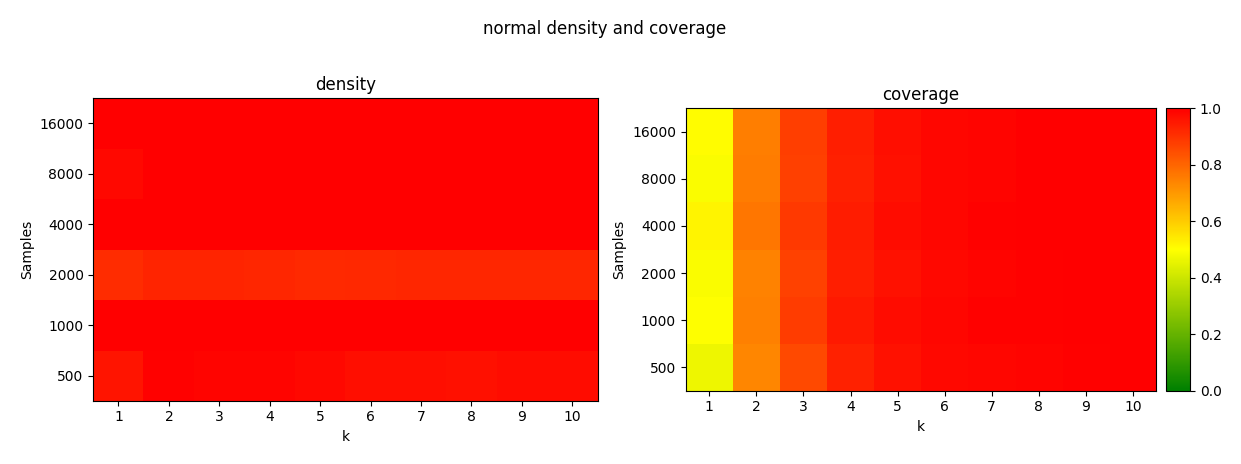
\includegraphics[width=0.8\textwidth]{../images/toyexperiments/kdim/normal_density_coverage.png} 
    \caption{Riproduzione delle heatmap presenti in Reliable Fidelity and Diversity Metrics for Generative Models \cite{3ReliableFidelityDiversityMetrics} per distribuzioni normali di dati}
\end{figure}

Come possiamo notare dai risultati in figura \ref{fig:toyexperiments-kdim-normal}, i risultati ottenuti sono molto simili a quelli presenti nel paper. Essendo le due distribuzioni di dati reali e generati identiche, una metrica che rispecchi tale somiglianza dovrebbe avere valori molto vicini ad \texttt{1.}, in particolar modo quando la dimensione del dataset è molto grande.
Un comportamento simile indicherebbe una buona robustezza della metrica rispetto a variazioni di \texttt{k}, ma come possiamo notare dai grafici, l'improved precision recall è molto più sensibile rispetto ai valori dell'iperparametro. 
Si può notare inoltre una sensibilità maggiore delle metriche al variare di \texttt{k} rispetto alla dimensione del dataset, i grafici sono infatti caratterrizati da colonne verticali di valori/colori molto simili.
La density dall'altra parte è molto più stabile, è però necessario ricordare che per distribuzioni di dati molto simili, non essendo normalizzata, ottenga valori persino maggiori di \texttt{1.}, portando la metrica a non essere molto significativa.
La coverage risulta anch'essa molto stabile, non dando valori molto diversi da \texttt{1.}, ad eccezione per \texttt{k = 1} con dimesione del dataset molto piccola.

C'è poi un altro elemento degno di nota che delude le aspettative ma che è perfettamente logico se si considera la natura delle metriche: l'improved precision-recall ottiene valori maggiori per dimensioni del dataset minori. Il motivo è che la metrica è basata sulla distanza fra i \texttt{k}-NN, e per dataset di dimensione ridotta, la distanza fra i \texttt{k}-NN è maggiore, portando a sovrastimare l'area del manifold di \(R\). Infatti il manifold ricopre un area che cresce quadraticamente rispetto alla distanza fra i campioni, e quando questi si fanno più radi il manifold cresce più velocemente andando ad includere più campioni (nonostante questi siano come detto più distanti fra loro).

Si riportano quindi i risultati per le due metriche ignorate dal paper sempre per distribuzioni normali di dati:

\begin{figure}[!ht]
    \centering
    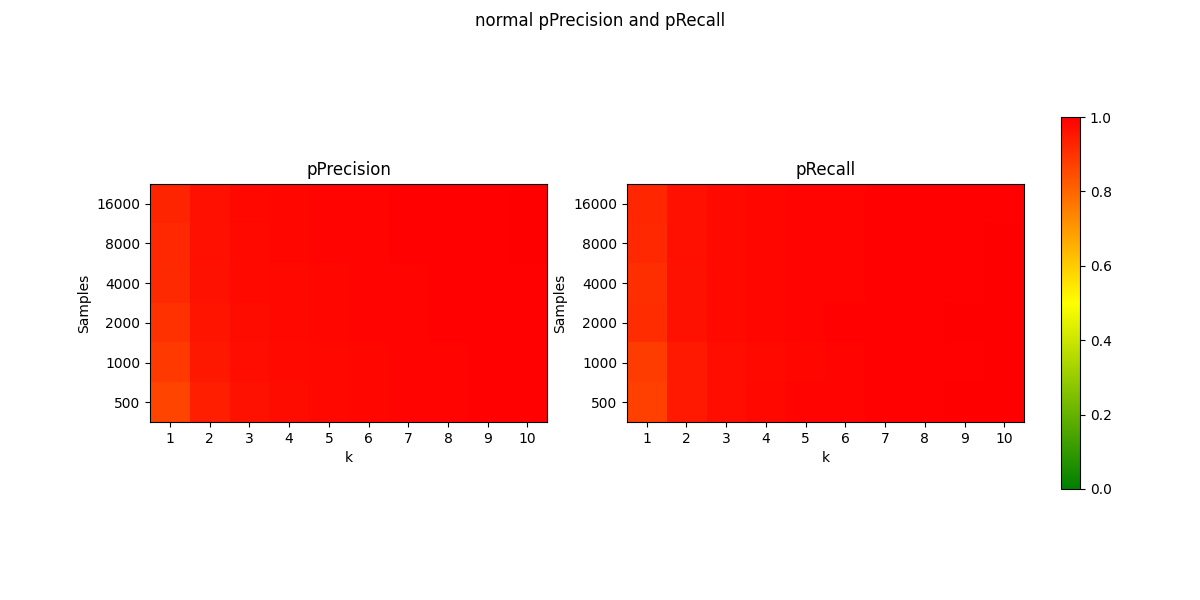
\includegraphics[width=0.8\textwidth]{../images/toyexperiments/kdim/normal_pPrecision_pRecall.png} 
    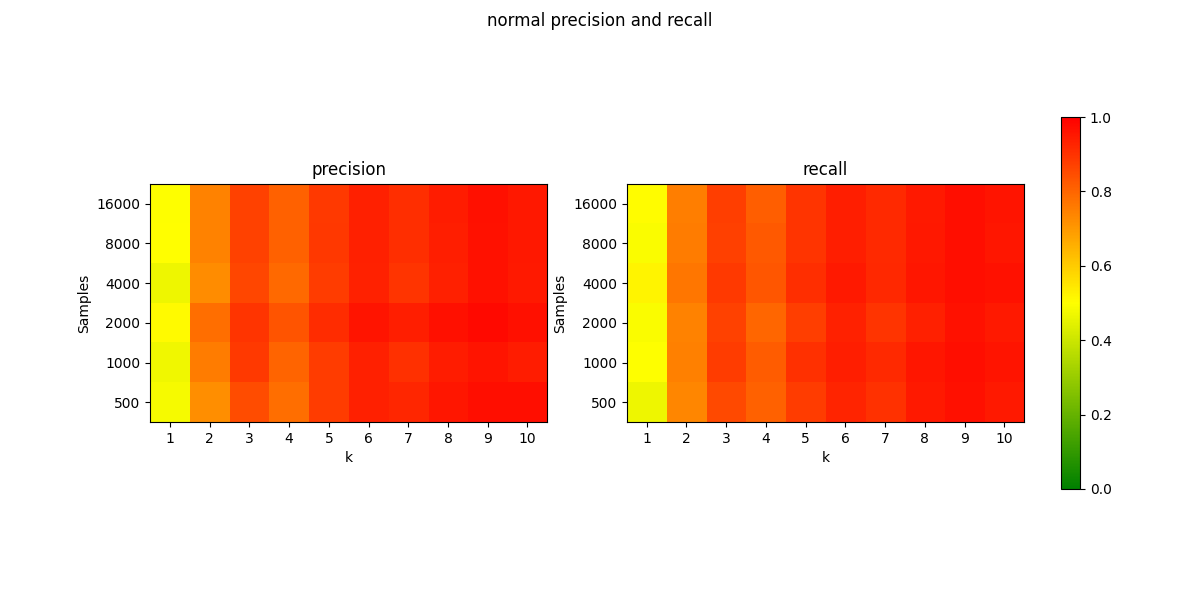
\includegraphics[width=0.8\textwidth]{../images/toyexperiments/kdim/normal_precision_recall.png} 
    \caption{Risultati per la probabibilistic precision-recall e la precision-recall coverage per distribuzioni normali di dati}
\end{figure}

In questo caso è apprezzabile l'uniformità di colore nei grafici della probabibilistic precision e recall, indice della corretta stima della sovrapposizione dei supporti dei dataset di eguale distribuzione.
Come per la density però, dobbiamo limitare i ragionamenti induttivi delle capacità della metrica di stimare la somiglianza fra due distribuzioni, a distribuzioni uguali. Questo vuol dire che con distribuzioni diverse la metrica potrebbe non risultare altrettanto sensibile e appunto continuare a dare valori alti quando non dovrebbe. 
Per la precision-recall coverage invece è interessante notare come per il valore di \texttt{k} consigliato in letteratura (\texttt{k = 3}) questa porti a una stima migliore persino che nel caso di \texttt{k} di valore superiore, dove teoricamente (esclusivamente per distribuzioni identiche), ci si aspetta stime migliori. 
Inoltre si può apprezzare la somiglianza fra i grafici della coverage e della precision-coverage, per i quali ricordiamo dalla teoria che con \texttt{k = 1} le due metriche risultano analiticamente identiche.

I risultati degli esperimenti su distribuzioni uniformi identiche sono i seguenti:

\begin{figure}[!ht]
    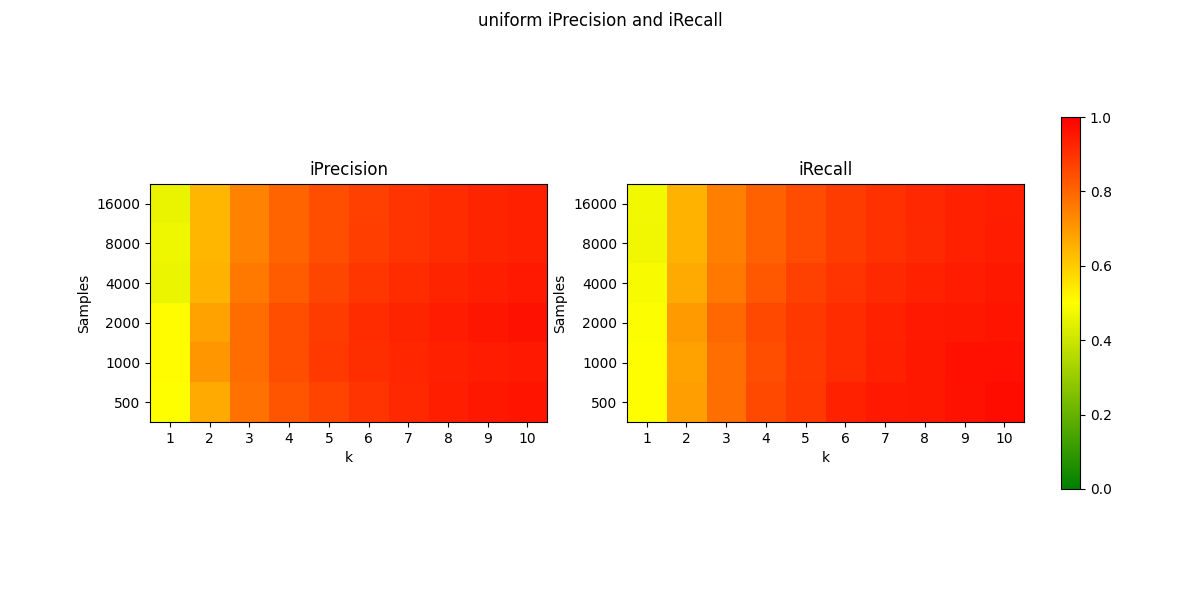
\includegraphics[width=0.5\textwidth]{../images/toyexperiments/kdim/uniform_iPrecision_iRecall.png} 
    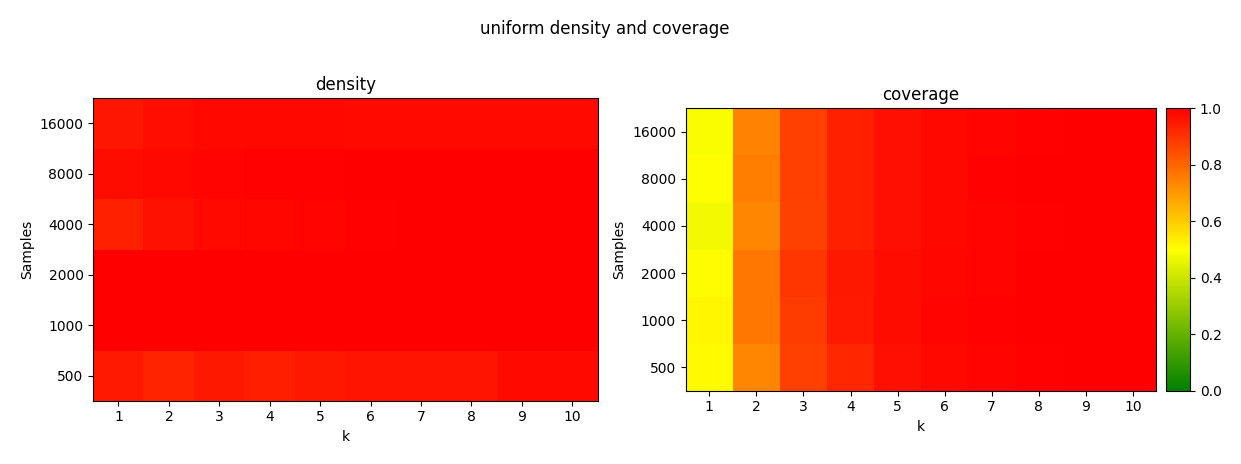
\includegraphics[width=0.5\textwidth]{../images/toyexperiments/kdim/uniform_density_coverage.png} 
    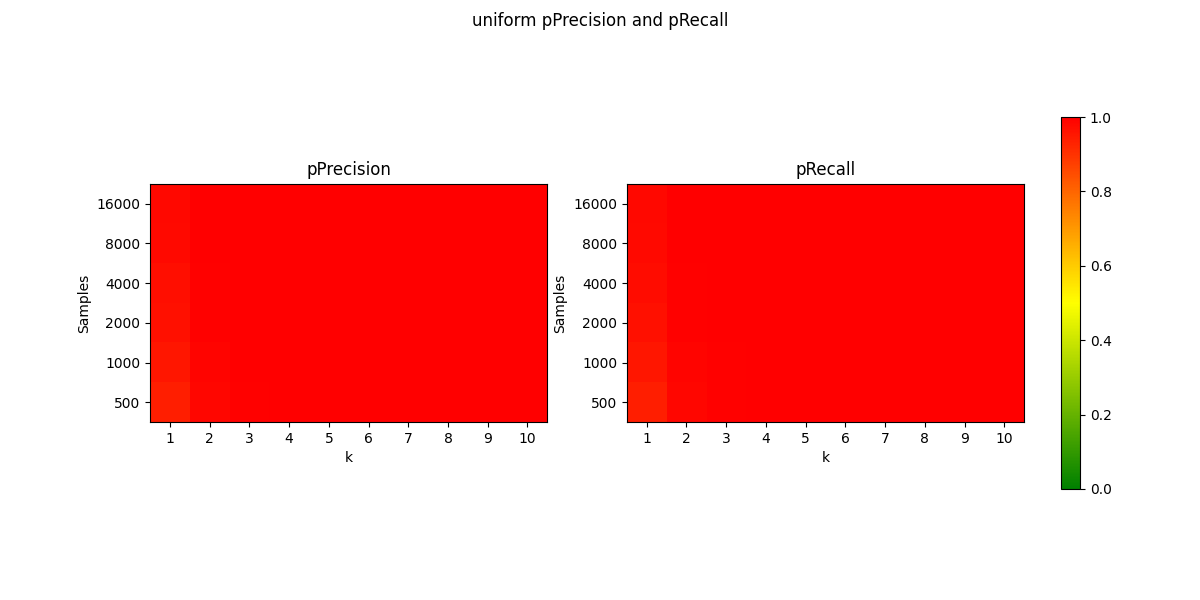
\includegraphics[width=0.5\textwidth]{../images/toyexperiments/kdim/uniform_pPrecision_pRecall.png}
    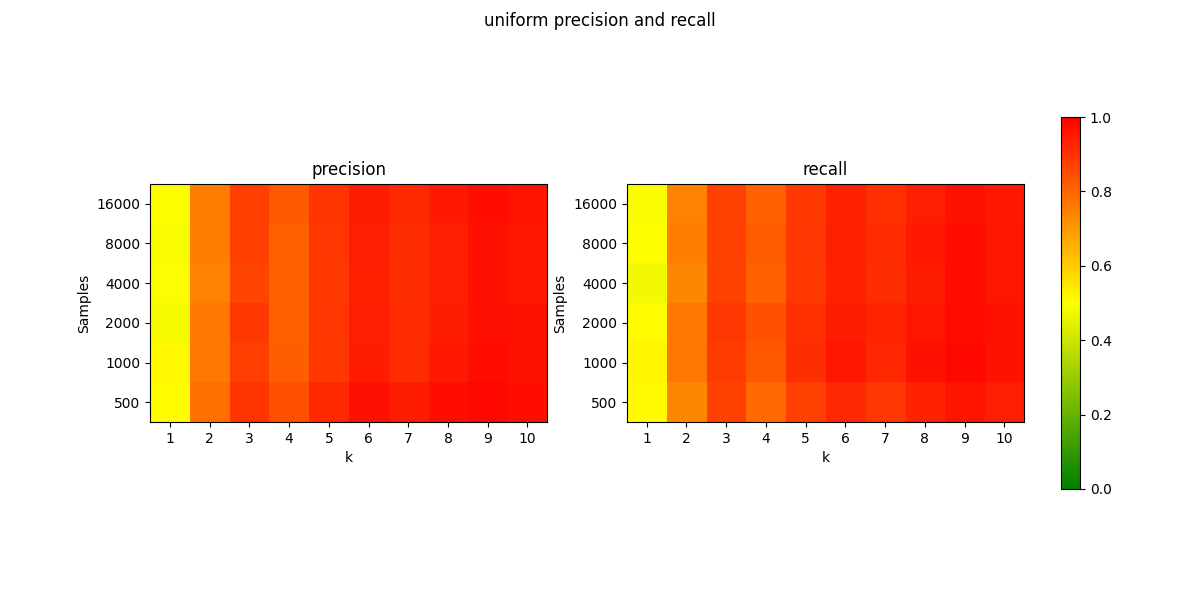
\includegraphics[width=0.5\textwidth]{../images/toyexperiments/kdim/uniform_precision_recall.png}
    \caption{Risultati per distribuzioni uniformi di dati identiche} 
\end{figure}

Come risulta a prima vista, non si discostano molto da i grafici ottenuti con distribuzioni normali. Possiamo quindi solo estendere le precedenti conclusioni a questa nuova distribuzione.
Unica eccezione è l'improved precision-recall che presenta risultati migliori in questo caso, segnalando una limitatezza della sensibilità in presenza di \texttt{k} con valori bassi e distribuzioni normali.

\subsection{Dimensione del dataset e dimensione dei dati}
\label{sec:res-dataset-data-dim}

Per quanto riguarda gli esperimenti sulla dimensione dei dati i risultati sono i seguenti:

\begin{figure}[!ht]
    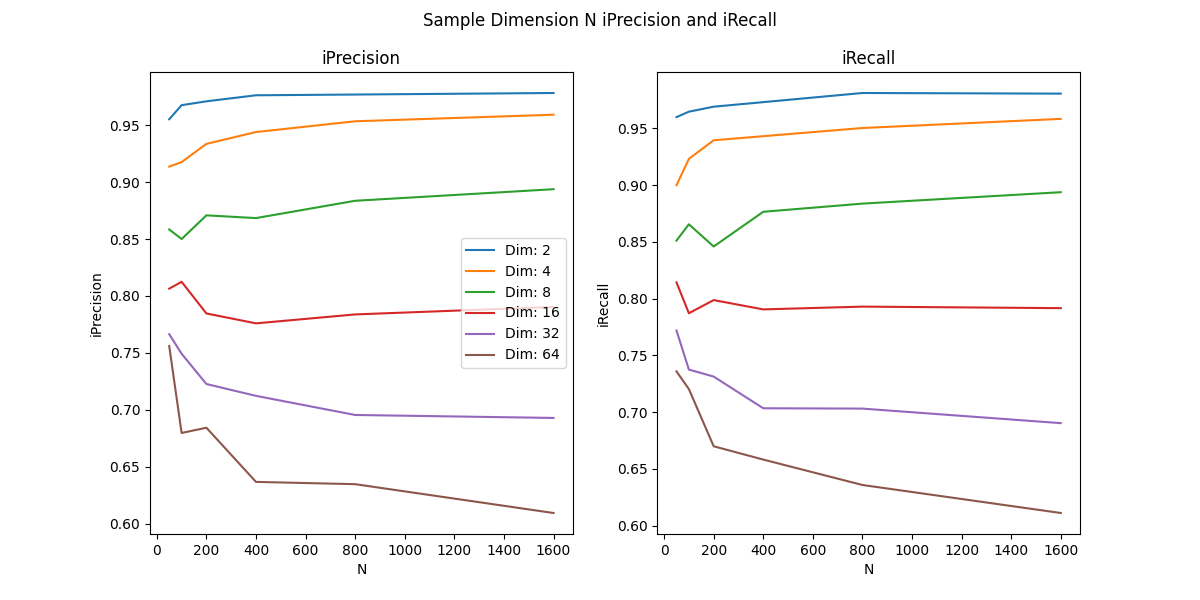
\includegraphics[width=0.5\textwidth]{../images/toyexperiments/ksampledim/sampleDimN_iPrecision_iRecall.png} 
    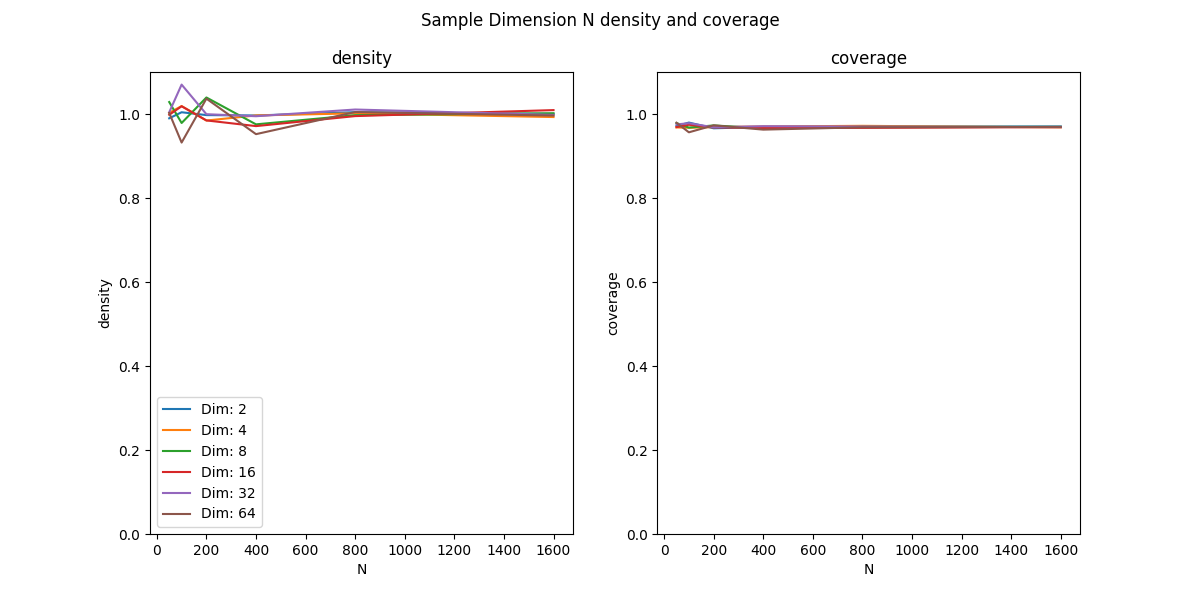
\includegraphics[width=0.5\textwidth]{../images/toyexperiments/ksampledim/sampleDimN_density_coverage.png} 
    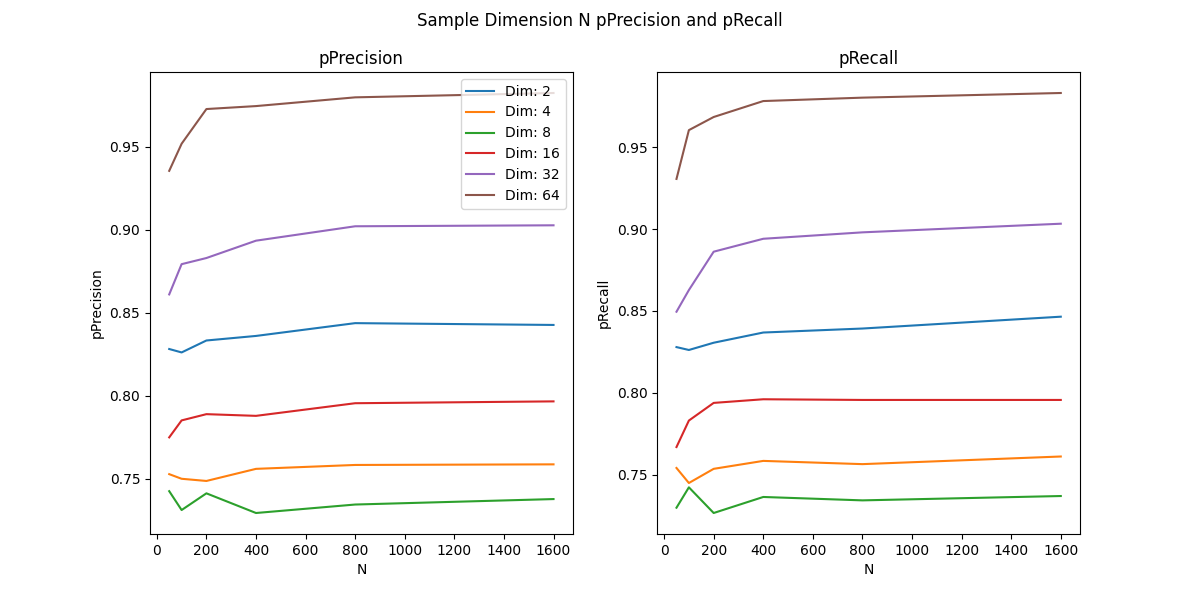
\includegraphics[width=0.5\textwidth]{../images/toyexperiments/ksampledim/sampleDimN_pPrecision_pRecall.png} 
    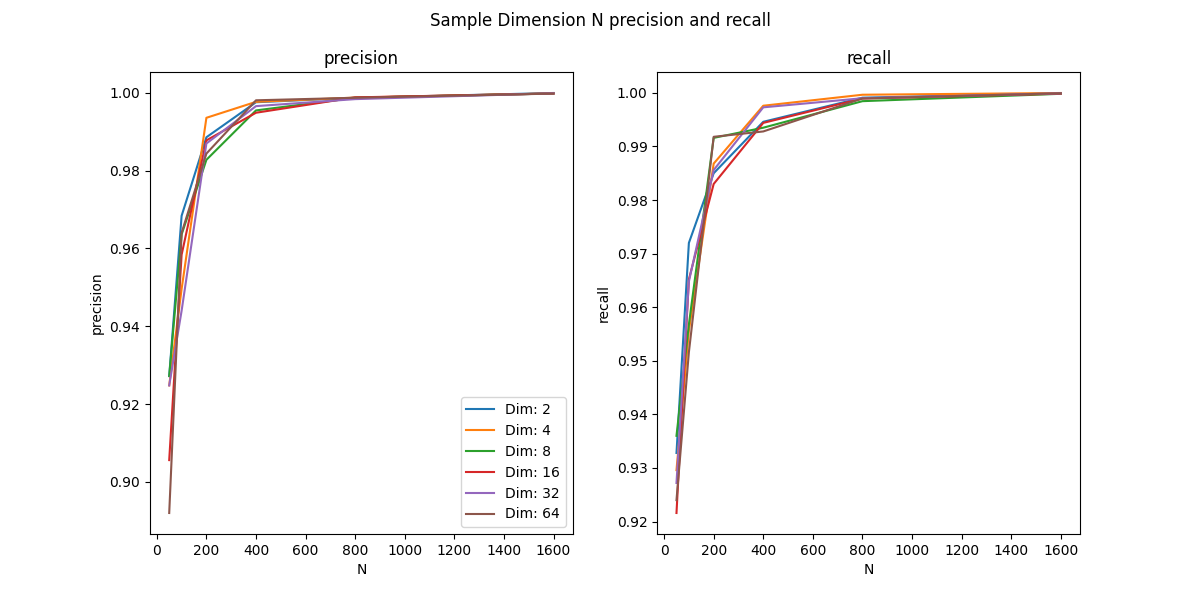
\includegraphics[width=0.5\textwidth]{../images/toyexperiments/ksampledim/sampleDimN_precision_recall.png} 
    \caption{Risultati per la variazione della dimensione dei dati, da sinistra a destra e dall'alto in basso le metriche sono: improved precision-recall, density-coverage, probabilistic precision-recall, precision-recall coverage}
\end{figure}

Le uniche due metriche che risultano sensibili alla variazione della dimensione dei dati sono la improved precision-recall e la probabibilistic precision-recall, mentre le altre due risultano molto stabili.
L'asse delle ascisse è stata limitata leggermente sopra a \texttt{1.} (\texttt{1.25}) possiamo quindi apprezzare visimamente una delle proprietà di cui abbiamo accennato nella sezione precedente e nel primo capitolo:
la density non essendo normalizzata presenta valori che superano il limite logico delle condiviso dalle altre metriche.

Per l'improved precision recall si individua la fragilità della metrica alla dimensione dei dati. Per dimensioni elevate, a parità di numero di campioni e di distribuzione, si registra valori di precision e recall inferiori.
Risulta infatti che per dati in \(\mathbb{R}^{64}\) i valori della metrica siano inferiori di circa 30 punti percentuale rispetto a i dati in  \(\mathbb{R}^{2}\). Si nota inoltre lo stesso difetto visto nella sezione precedente \ref{sec:res-k-dataset-dim}, ovvero che la metrica risulta produrre valori migliori per dimensioni dei dati minori.
Le ragioni sono le stesse, la distanza interna fra i dati è maggiore e quindi il manifold viene sovrastimato.

Per la probabilistic precision recall è sempre presente questa fragilità, ma non è ben chiaro come la dimensione dei dati sia legata agli effettivi risultati della metrica, risulta infatti che per le due dimensioni dei dati maggiori
testate i valori della metrica siano migliori ma con essi è presente anche la dimensione dei dati minore testata, mentre per \(\mathbb{R}^{8}\) otteniamo la stima più bassa.

\subsection{Outliers}
\label{sec:res-outliers}

I casi di studio, come detto nel capitolo precedente sono tre: valori della metrica per distribuzioni normali di dati reali e generate, con la distribuzione dei dati generati centrata nei diversi valori dell'ordinata senza outliers, con outliers nei dati reali e con outliers nei dati generati.

I risultati ottenuti per l'improved precision-recall sono riportati nell immagine \ref{fig:toyexperiments-outliers}. 

\begin{figure}[!ht]
    \label{fig:toyexperiments-outliers}
    \centering
    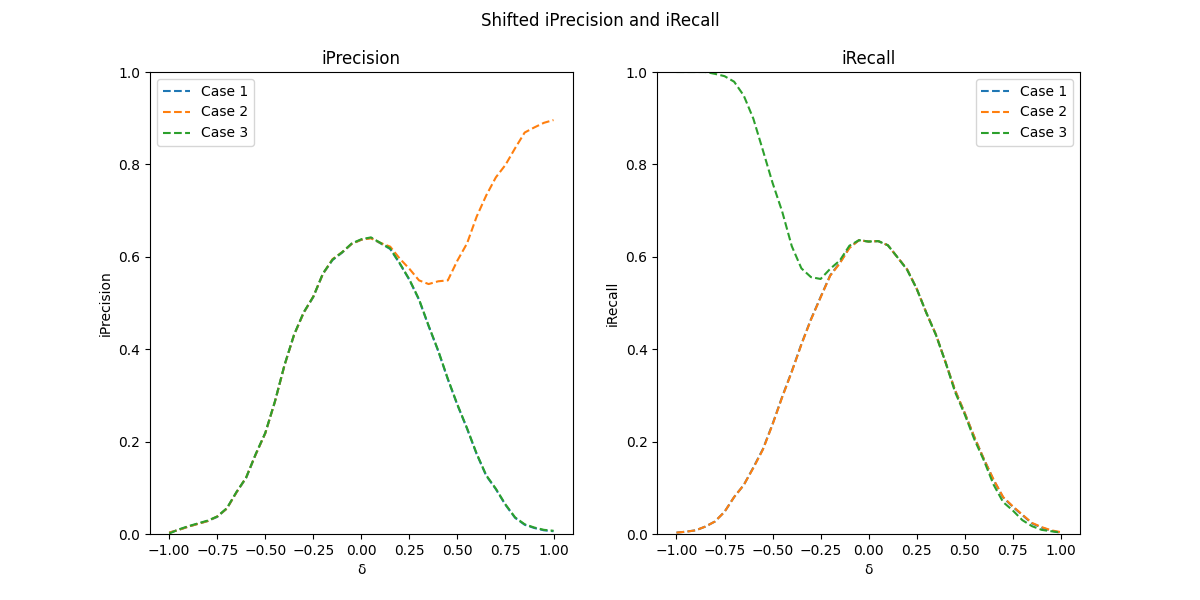
\includegraphics[width=0.8\textwidth]{../images/toyexperiments/outliers/shift_iPrecision_iRecall.png} 
    \caption{Risultati per la resistenza della improved precision-recall alla presenza di outliers nei dati, riprodotto da Reliable Fidelity and Diversity Metrics for Generative Models \cite{3ReliableFidelityDiversityMetrics}}
\end{figure}

È possibile notare che i risultati ottenuti rispettano quanto atteso dalla letteratura. La metrica risulta essere molto sensibile alla presenza di outliers nei dati.
In particolare la precision risulta essere estremamente sensibile alla presenza di outliers nei dati \textbf{reali}, poichè questi vanno a determinare una sovrastimare dell'area del manifold di \(R\), dall'altra parte 
la recall risulta essere molto sensibile alla presenza di outliers nei dati \textbf{generati}, poichè in questo caso si va a sovrastimare l'area del manifold di \(G\).
Un singolo dato outlier può far variare la metrica dell'80\% rispetto al caso senza outliers.
Un altro problema grave delle due metriche è che quando lo shift fra le due distribuzioni è \texttt{0.} la metrica è molto più bassa di \texttt{1.}, paradossalmente viene registrato un valore maggiore dei manifold per distribuzioni con media spostata rispetto a distribuzioni con media centrata.

I risultati ottenuti per la density-coverage sono i seguenti:

\begin{figure}[!ht]
    \centering
    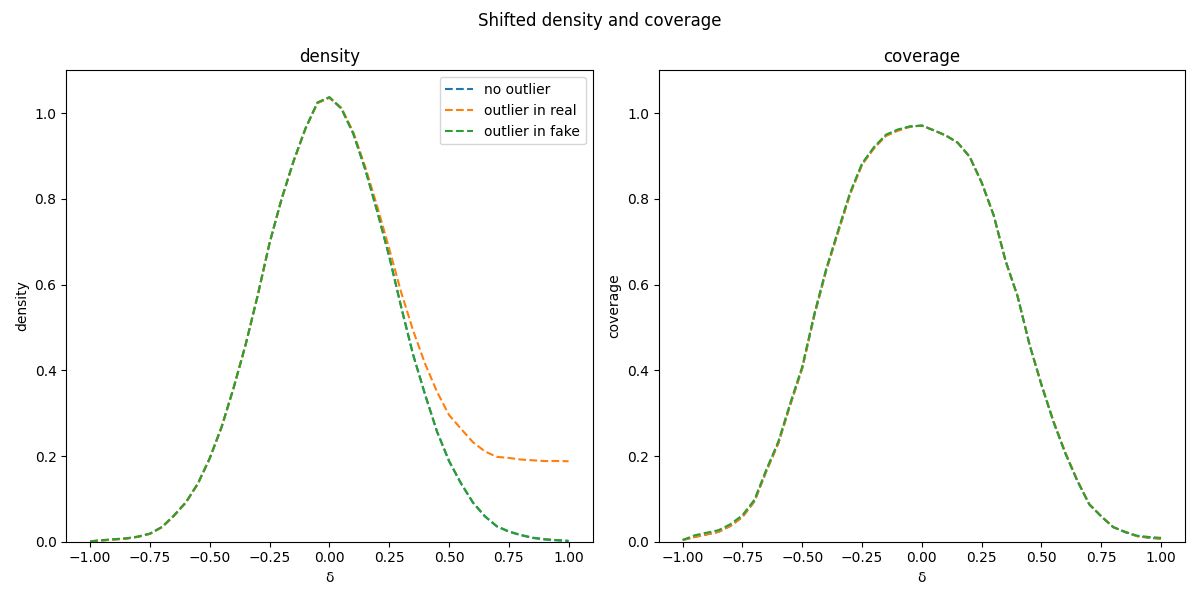
\includegraphics[width=0.8\textwidth]{../images/toyexperiments/outliers/shift_density_coverage.png} 
    \caption{Risultati per la resistenza della density-coverage alla presenza di outliers nei dati, riprodotto da Reliable Fidelity and Diversity Metrics for Generative Models \cite{3ReliableFidelityDiversityMetrics}}
\end{figure}

Ancora una volta i risultati ottenuti rispettano quanto atteso dalla letteratura. La metrica risulta essere molto robusta alla presenza di outliers nei dati.
La density è leggermente influenzata dalla presenza di outliers nei dati reali, ma non in maniera significativa, mentre la coverage non risente della presenza di outliers sia nei dati reali che nei dati generati.
Al contrario dell'improved precision recall, la density e la coverage hanno valori molto vicini a \texttt{1.} quando lo shift fra le due distribuzioni è \texttt{0.} (la density non essendo normalizzata ha valori maggiori di \texttt{1.}).

Per le altre due metriche non indagate nel paper i risultati sono i seguenti:

\begin{figure}[!ht]
    \centering
    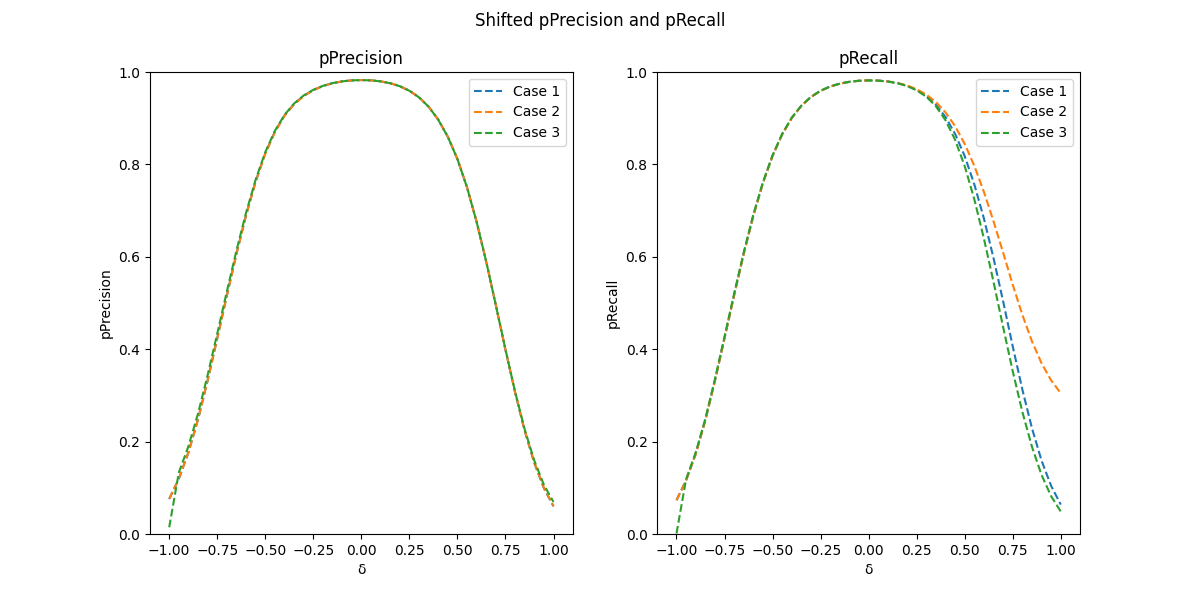
\includegraphics[width=0.8\textwidth]{../images/toyexperiments/outliers/shift_pPrecision_pRecall.png} 
    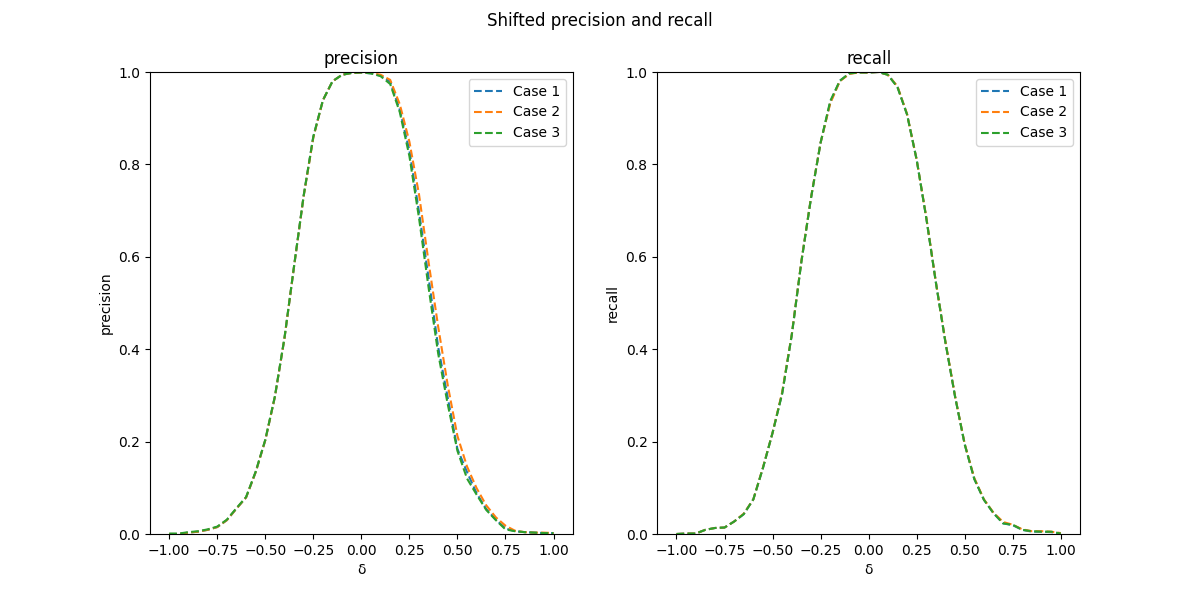
\includegraphics[width=0.8\textwidth]{../images/toyexperiments/outliers/shift_precision_recall.png} 
    \caption{Risultati per la resistenza della probabibilistic precision-recall e della precision-recall coverage alla presenza di outliers nei dati}
\end{figure}

Come per la density e coverage, le due metriche più recenti risultano essere molto robuste alla presenza di outliers nei dati e misurano correttamente la sovrapposizione dei manifold delle due distribuzioni in assenza di shift.
Data la diversa natura delle due metriche, la probabibilistic precision-recall presenta valori più alti quando lo shift è non nullo.

\subsection{Comparazione con implementazioni esistenti e riproduzione delle pr-curves}

Come avevamo anticipato nell'introduzione dei ToyData experiments, abbiamo verificato che le implementazioni presentate nei vari paper presi in esame riportassero risultati conformi a quelli ottenuti con la nostra implementazione.
Per fare ciò, oltre a riprodurre esperimenti simili a quelli presenti nei paper e confrontato i grafici come visto sino ad adesso, abbiamo verificato numericamente che i valori delle metriche fossero effettivamente gli stessi.
Una rapida presa visione del codice sorgente ha permesso di verificare delle differenze implementative che però sono risultate indifferenti se non in termini di complessità computazionale.

Per quanto riguarda le implementazioni di improved precision-recall \cite{2ImprovedPrecisionRecall} i risultati ottenuti sono identici per tutte e tre le distribuzioni di dati presi in analisi.

Per le implementazioni di improved precision-recall e density-coverage \cite{3ReliableFidelityDiversityMetrics} i risultati ottenuti sono identici per tutte e tre le distribuzioni di dati presi in analisi.

Per le implementazioni di probabilistic precision-recall \cite{4ProbabilisticPrecisionRecall} i risultati ottenuti differiscono alla 15esima cifra significativa per tutte e tre le distribuzioni di dati presi in analisi.
Tale differenza non è significativa e può essere attribuita a errori numerici dovuti alla precisione di calcolo delle macchine. Per il calcolo della probabibilistic precision-recall è necessario anche il calcolo della \(\rho(\Phi)\) che è come visto nel capitolo 1 \ref{eq:rho} una media delle \texttt{k}-NN distances,
e nei nostri esperimenti risulta che anche la misura di questa distanza risulta essere equivalente a quella calcolata dalle implementazioni dei papers.

Passiamo ora alla comparazione delle pr-curves. In questo caso le pr-curves riprodotte dipendevano dalla scelta del parametro \texttt{k}, dallo shift fra le due distribuzioni e dallo split del traing set e del test set.
Per i dataset normali con split del 50\% abbiamo ottenuto i seguenti risultati:

\begin{figure}[!ht]
    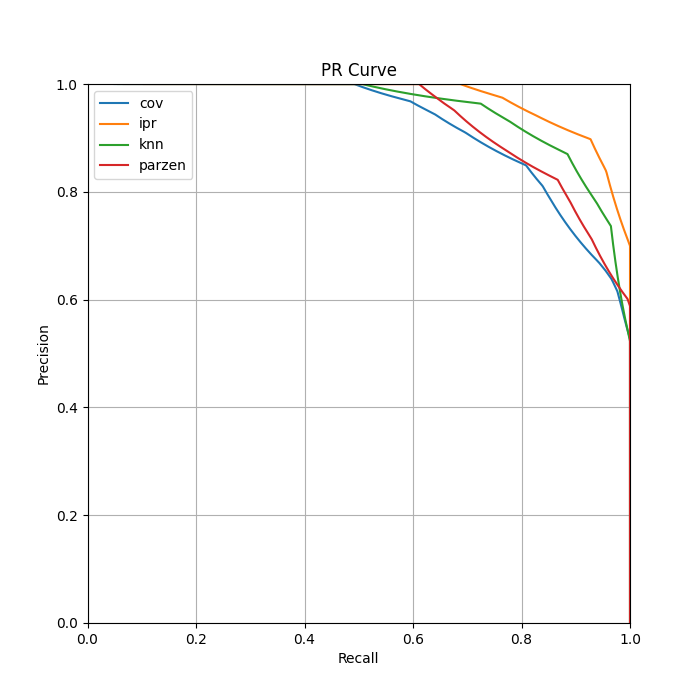
\includegraphics[width=0.5\textwidth]{../images/toyexperiments/prcurves/PRCurve_k4_s1.png} 
    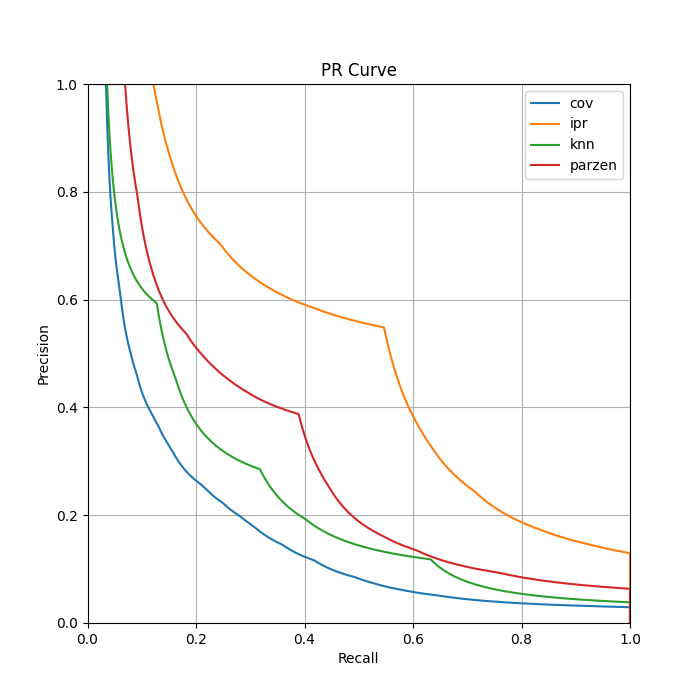
\includegraphics[width=0.5\textwidth]{../images/toyexperiments/prcurves/PRCurve_k4_s3.png}
    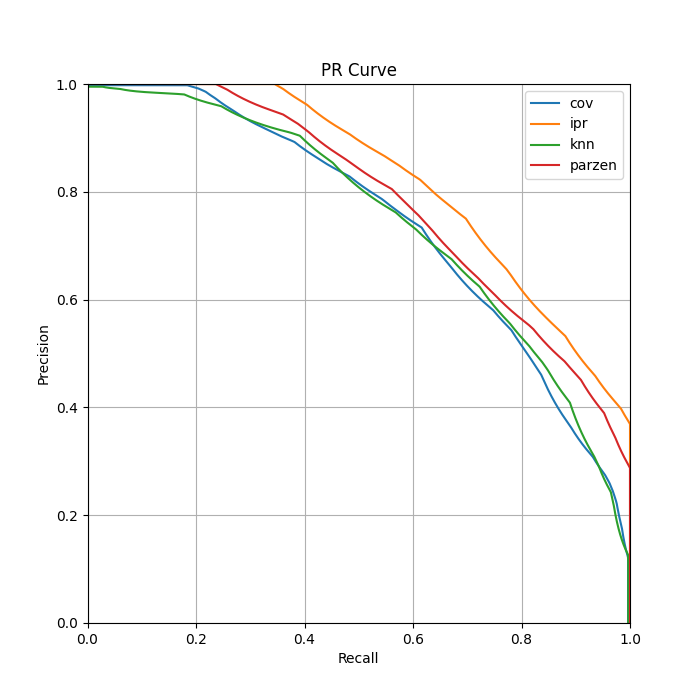
\includegraphics[width=0.5\textwidth]{../images/toyexperiments/prcurves/PRCurve_ksqrt_s1.png} 
    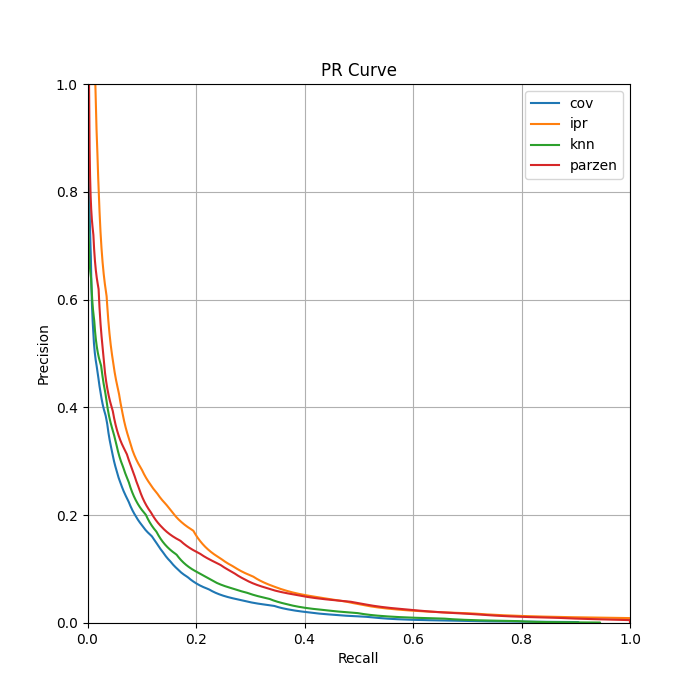
\includegraphics[width=0.5\textwidth]{../images/toyexperiments/prcurves/PRCurve_ksqrt_s3.png}
    \caption{Risultati per le pr-curves per dataset normali con split del 50\%} 
\end{figure}


Per i dataset normali senza split abbiamo ottenuto i seguenti risultati:

\begin{figure}[!ht]
    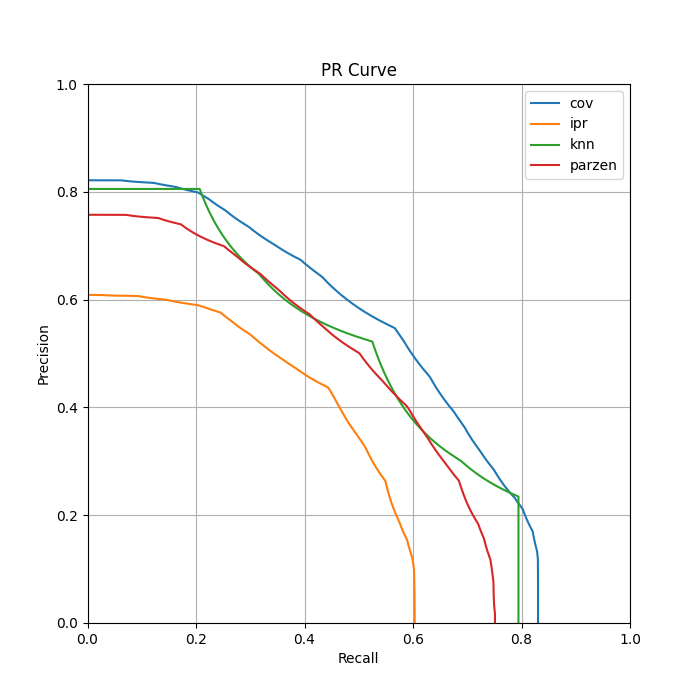
\includegraphics[width=0.5\textwidth]{../images/toyexperiments/prcurves/PRCurve_nosplit_k4_s1.png}
    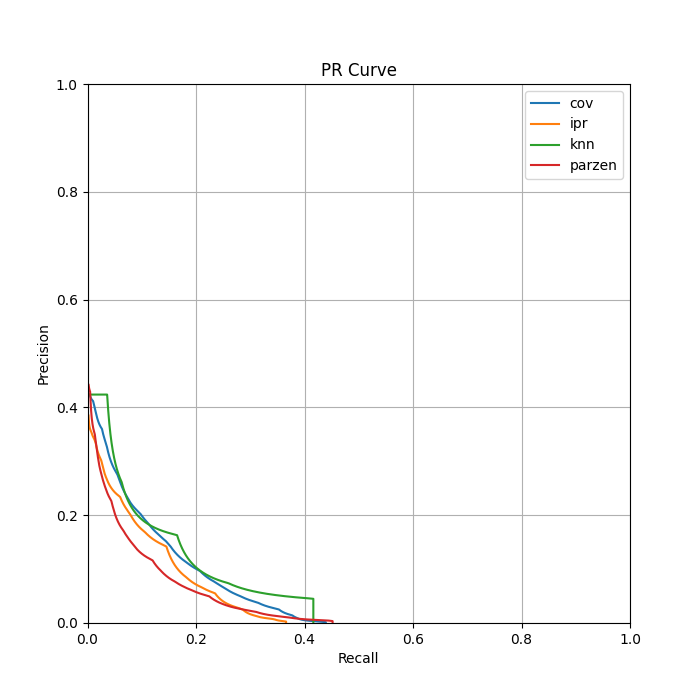
\includegraphics[width=0.5\textwidth]{../images/toyexperiments/prcurves/PRCurve_nosplit_k4_s3.png}
    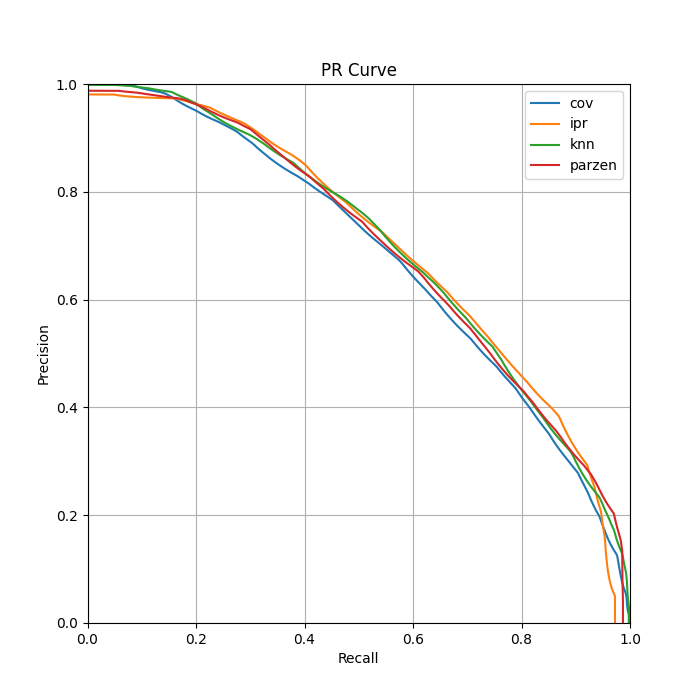
\includegraphics[width=0.5\textwidth]{../images/toyexperiments/prcurves/PRCurve_nosplit_ksqrt_s1.png}
    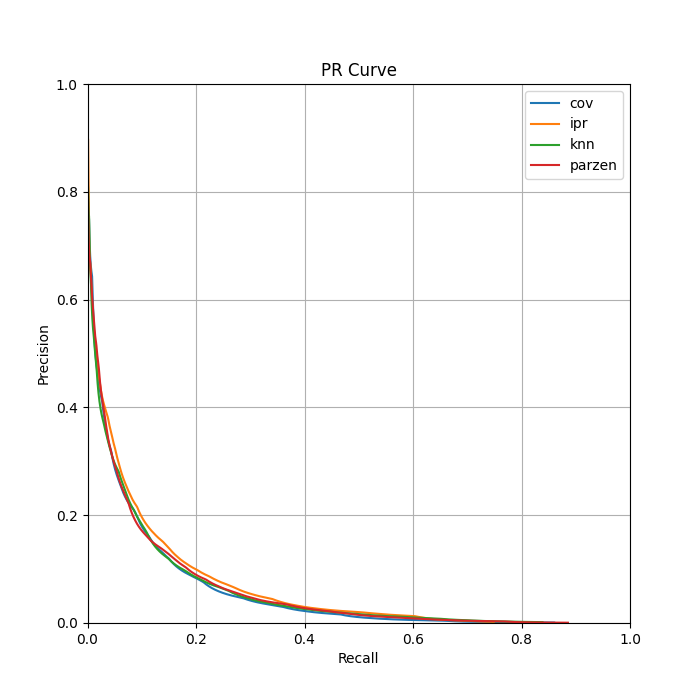
\includegraphics[width=0.5\textwidth]{../images/toyexperiments/prcurves/PRCurve_nosplit_ksqrt_s3.png}
    \caption{Risultati per le pr-curves per dataset normali senza split}
\end{figure}

Anche in questo caso i risultati ottenuti sono conformi a quelli attesi e presenti nei paper. Le conclusioni che si possono trarre sono pertanto le stesse di quelle presenti nei paper, vale a dire che si nota una maggiore stabilità delle pr-curves in presenza di uno split del dataset e con \texttt{k = \(\sqrt{|\Phi|}\)}.

\section{Risultati degli esperimenti su dataset reali}

\subsection{Butterflies}
\label{subsec:res-butterflies}

Prima di condurre gli esperimenti per identificare se le metriche possano operare correttamente da filtro per la selezione di dati generati di alta qualità, abbiamo condotto degli esperimenti preliminari per studiare il dominio in cui avrebbero operato le metriche.
In particolare abbiamo analizzato le kde delle divese caratterristiche proposte per le distanze inter e intra set. L'obbiettivo era quello di verificare che tali caratterristiche fossero sufficientemente descrittive per poter distinguere dati generati di alta qualità da dati generati di bassa qualità.
I risultati ottenuti sono i seguenti:

\begin{figure}[!ht]
    \centering
    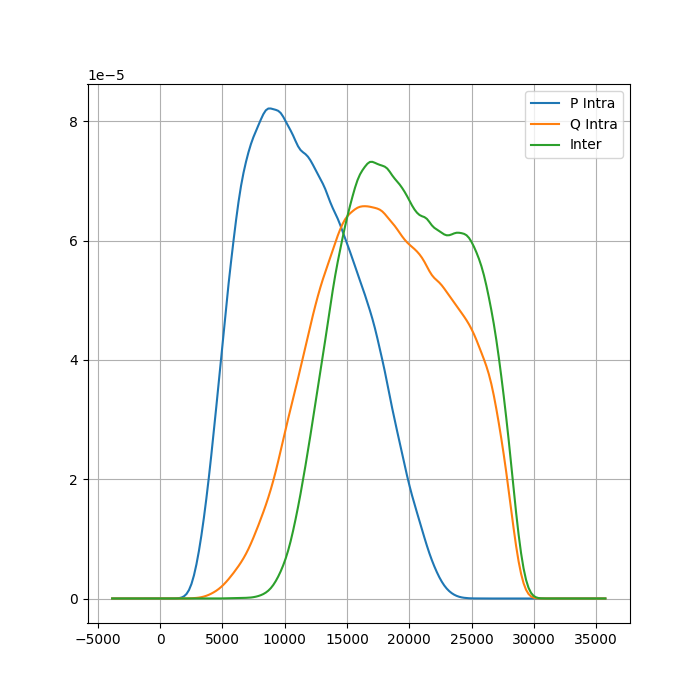
\includegraphics[width=0.3\textwidth]{../images/realworldexperiments/butterflies/kde/kde_grayscale_histogram.png}
    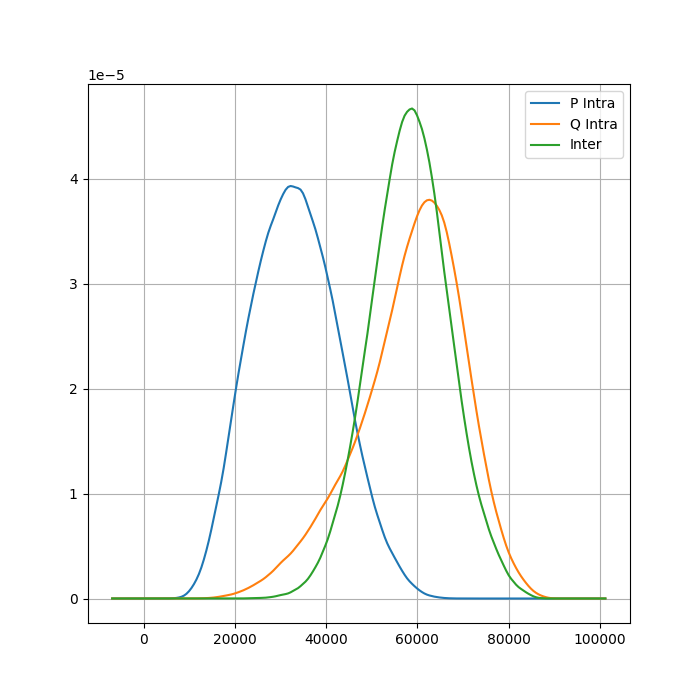
\includegraphics[width=0.3\textwidth]{../images/realworldexperiments/butterflies/kde/kde_hsv_histogram.png}
    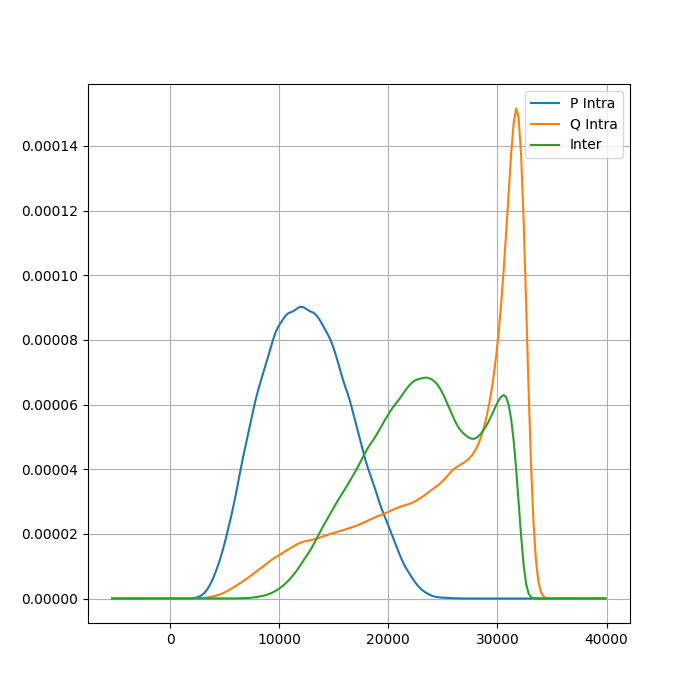
\includegraphics[width=0.3\textwidth]{../images/realworldexperiments/butterflies/kde/kde_hue_histogram.png}
\end{figure}
\begin{figure}[!ht]
    \centering
    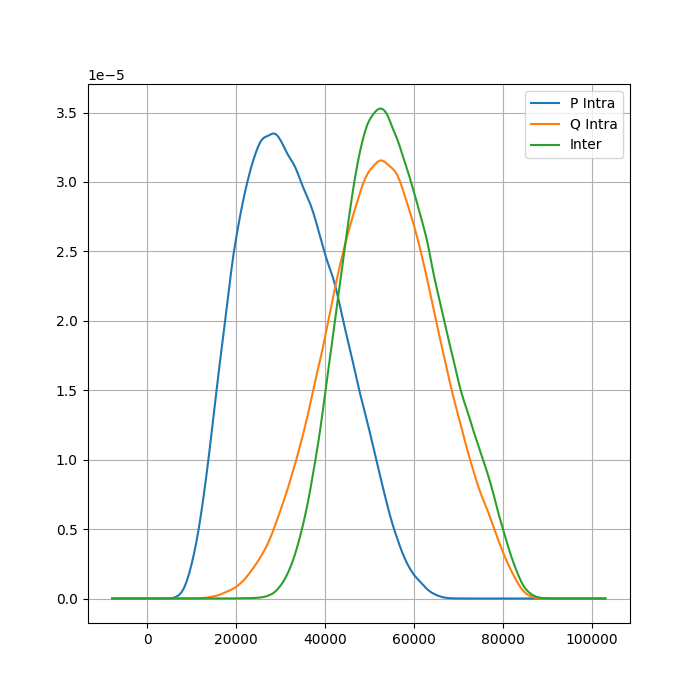
\includegraphics[width=0.3\textwidth]{../images/realworldexperiments/butterflies/kde/kde_rgb_histogram.png}
    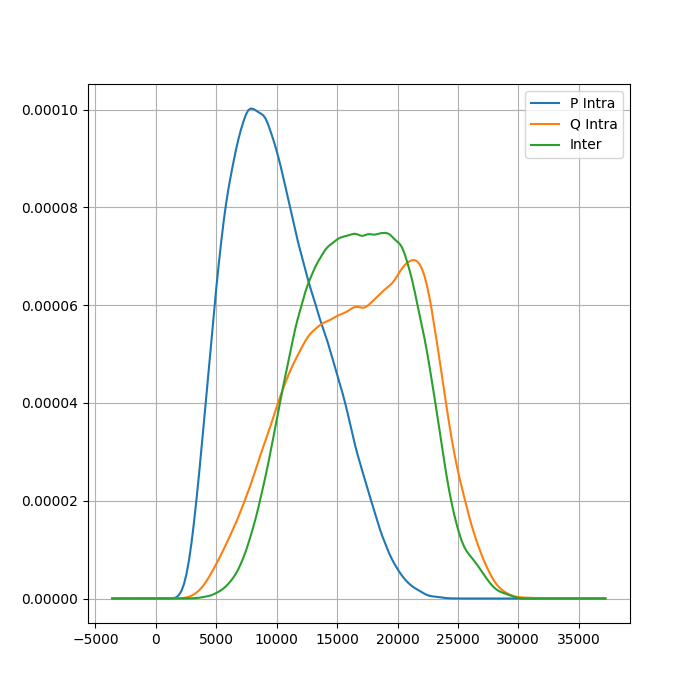
\includegraphics[width=0.3\textwidth]{../images/realworldexperiments/butterflies/kde/kde_saturation_histogram.png}
    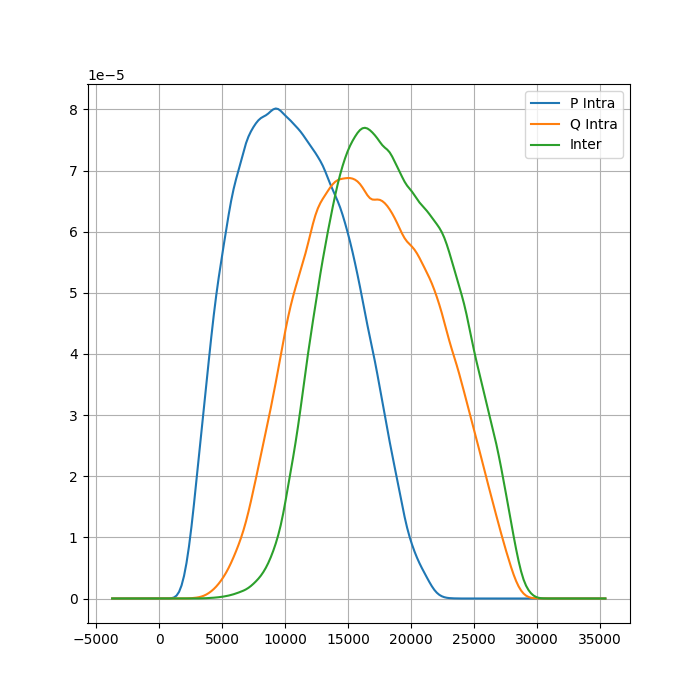
\includegraphics[width=0.3\textwidth]{../images/realworldexperiments/butterflies/kde/kde_value_histogram.png}
    \caption{l'ordine delle immagini da sinistra a destra e dall'alto in basso è: grayscale, hsv, hue, rgb, saturation, value}
\end{figure}

L'analisi delle Kernel Density Estimation (KDE) applicata alle distanze intra-set per i campioni reali e quelli generati evidenzia una limitata sovrapposizione tra le distribuzioni. Le distanze intra-set dei dati reali si concentrano, come ci si potrebbe aspettare intorno a valori più bassi, mentre quelle dei dati generati mostrano una maggiore dispersione, con una tendenza verso distanze più elevate. Questo comportamento implica che i campioni generati, anche quelli più vicini al manifold dei dati reali, difficilmente raggiungono la stessa compattezza dei campioni reali.

Per ogni tipo di istogramma analizzato, sono stati selezionati i 5 falsi positivi (immagini generate che ricadono nel manifold dei dati reali) con le distanze più elevate dai dati reali e i 5 veri positivi (immagini generate correttamente che ricadono sotto il manifold dei dati reali) con le distanze minori. Questi sono stati confrontati con le rispettive immagini reali più vicine, per un totale di 20 immagini per ogni istogramma. 
I risultati sono nella figura \ref{fig:realworldexperiments-butterflies} che segue.

\begin{figure}[!ht]
    \label{fig:realworldexperiments-butterflies}
    \centering
    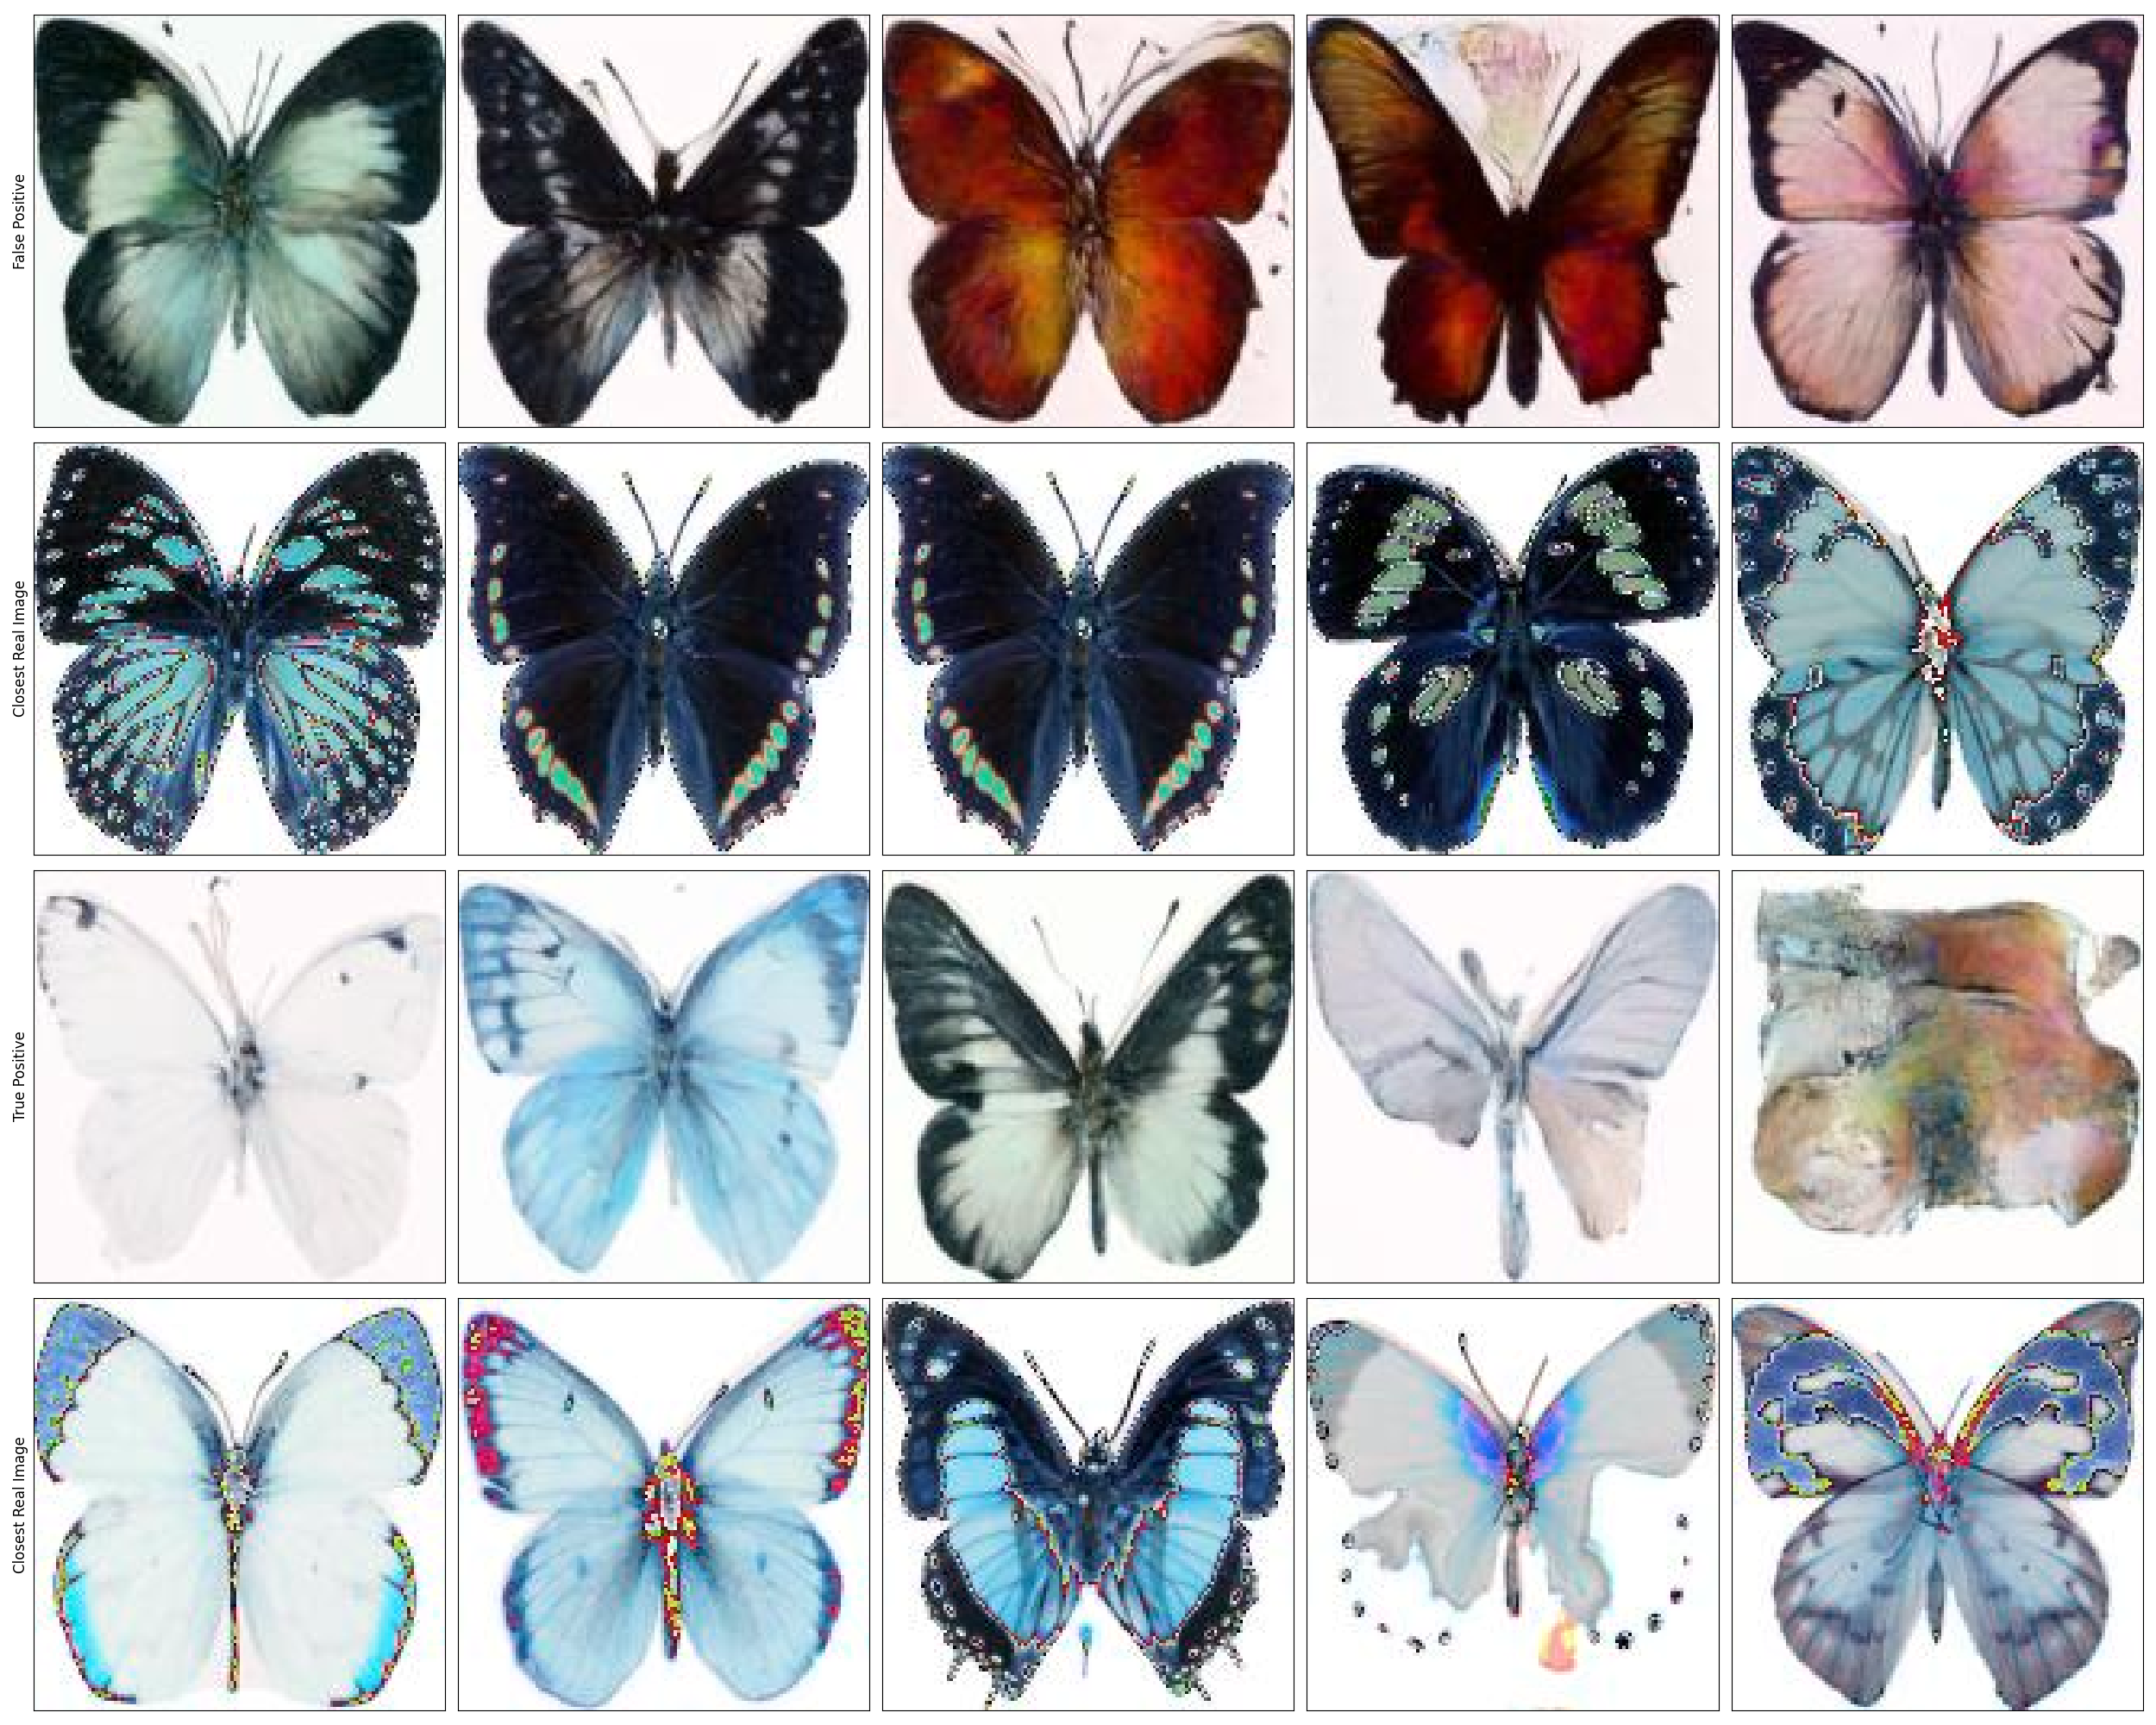
\includegraphics[width=0.45\textwidth]{../images/realworldexperiments/butterflies/examples/fp_grayscale_histogram.png}
    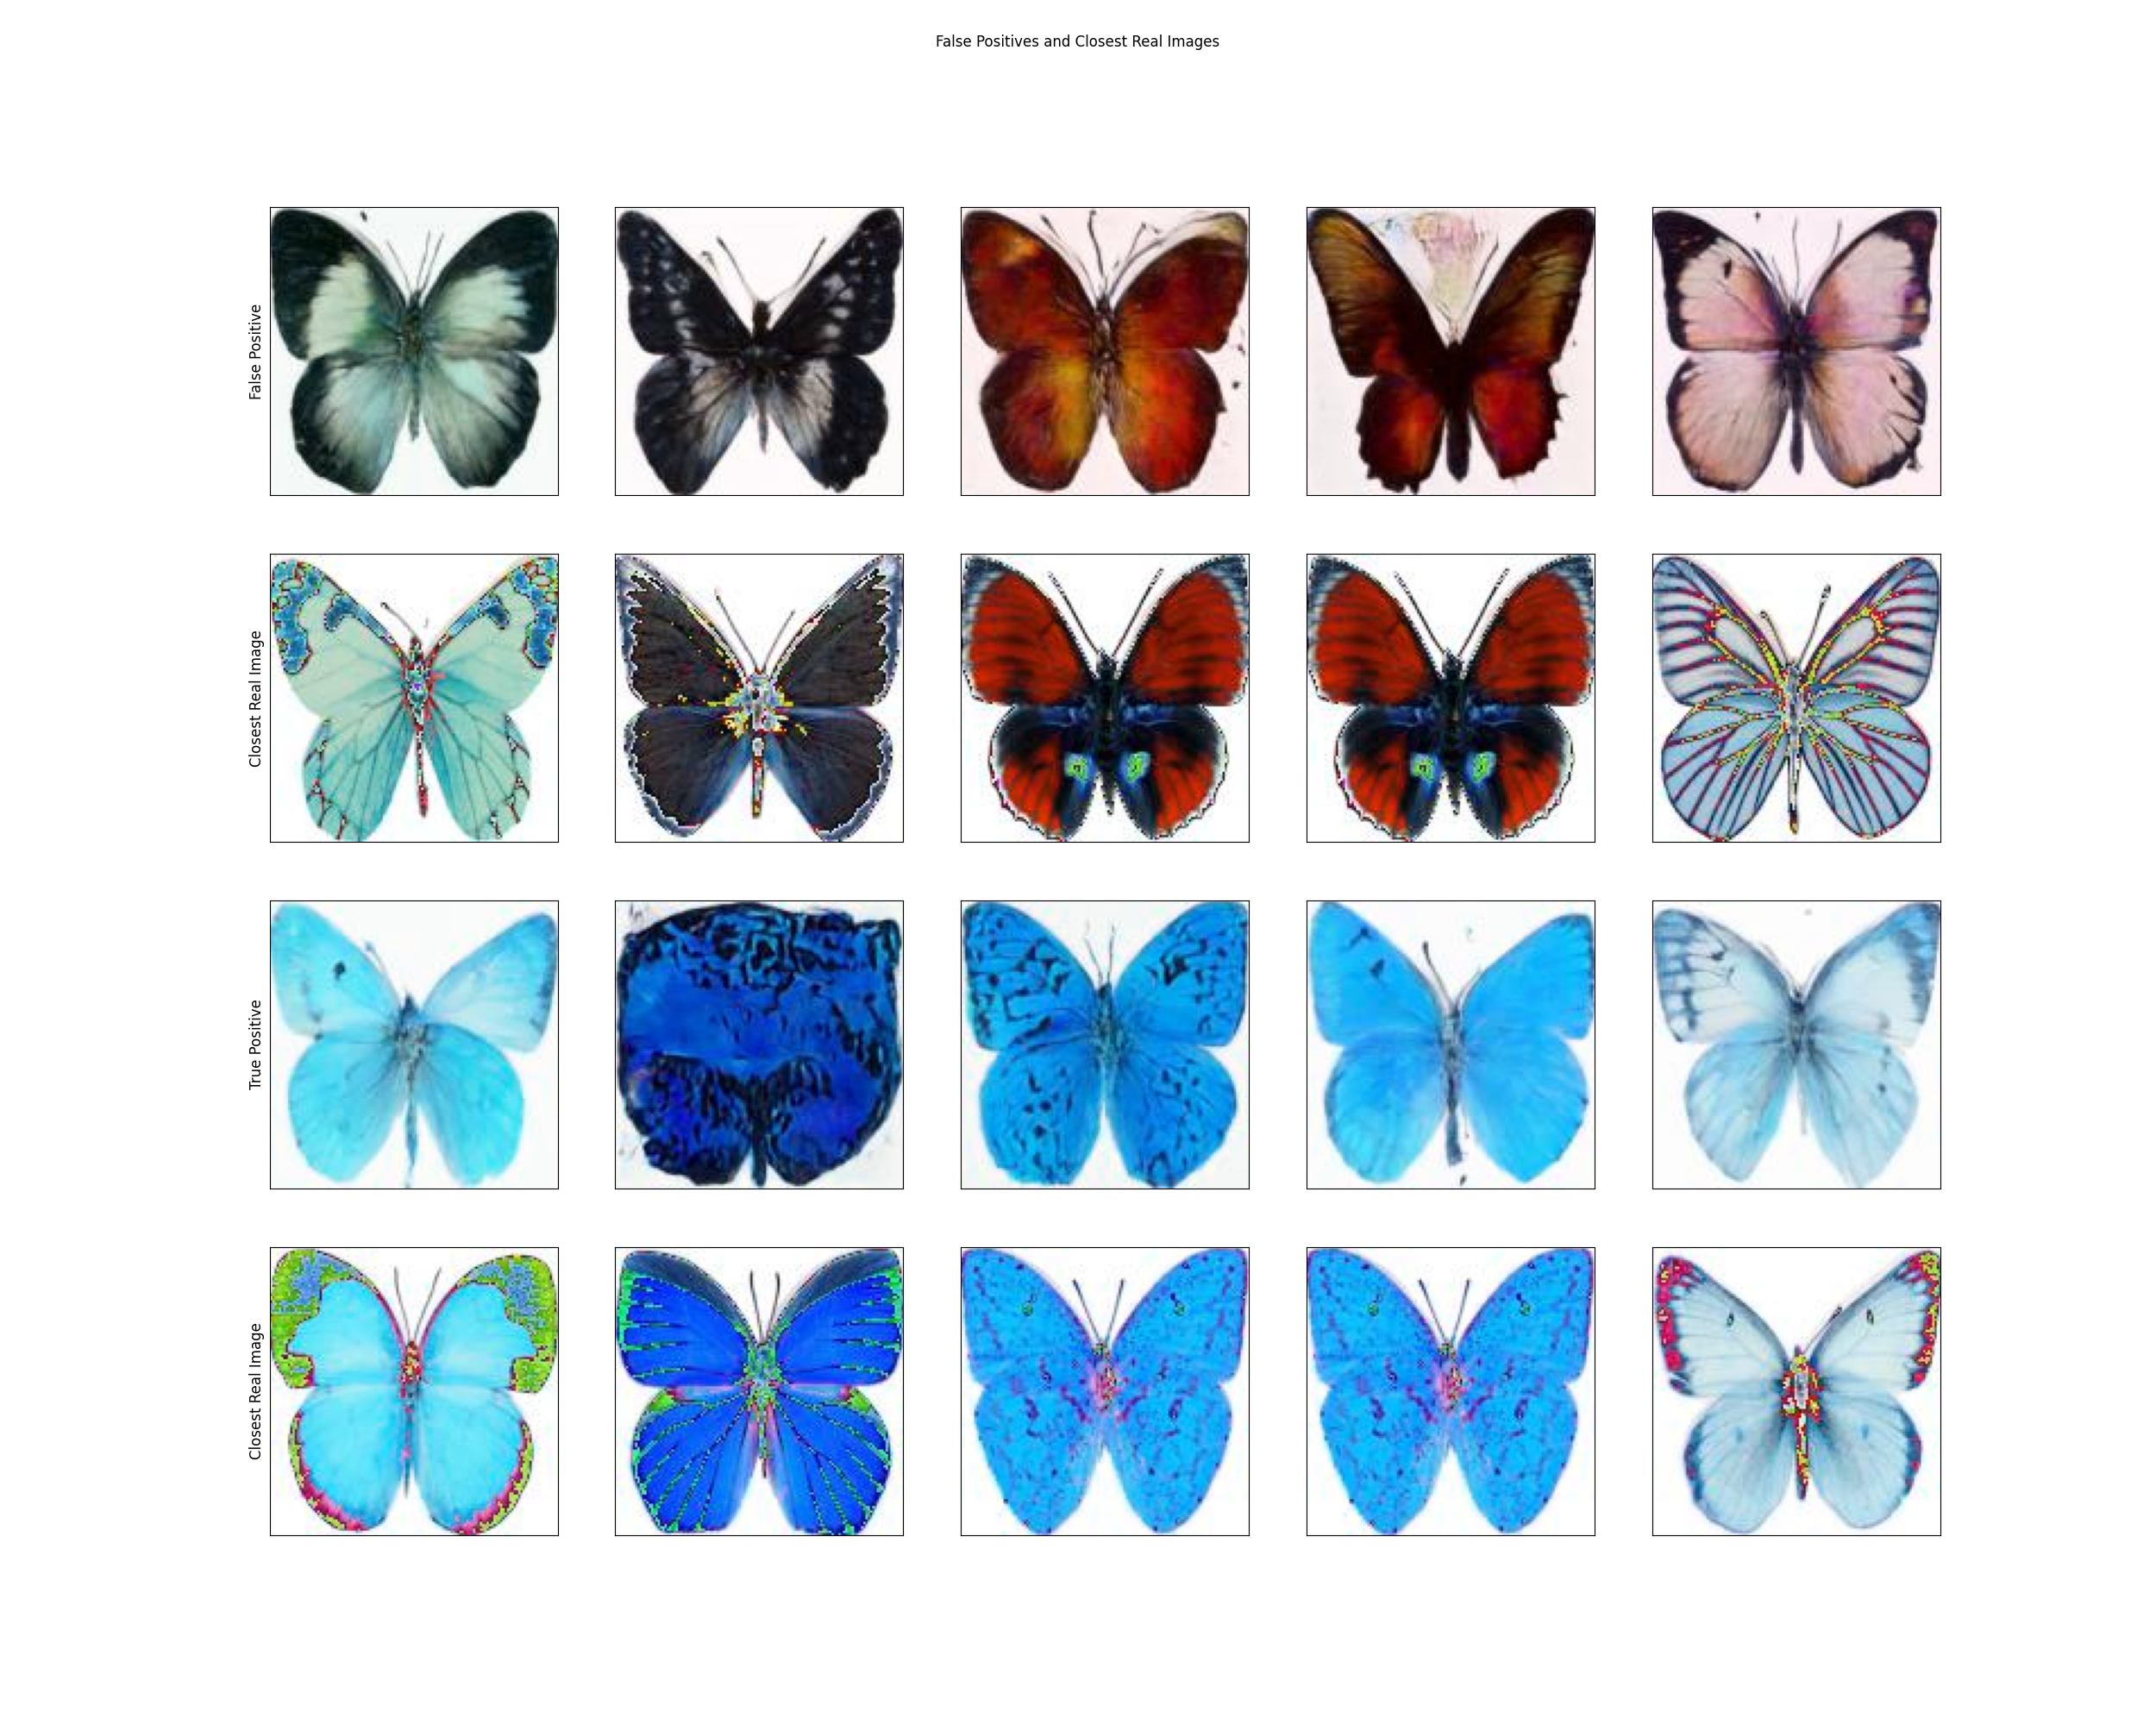
\includegraphics[width=0.45\textwidth]{../images/realworldexperiments/butterflies/examples/fp_hsv_histogram.png}
    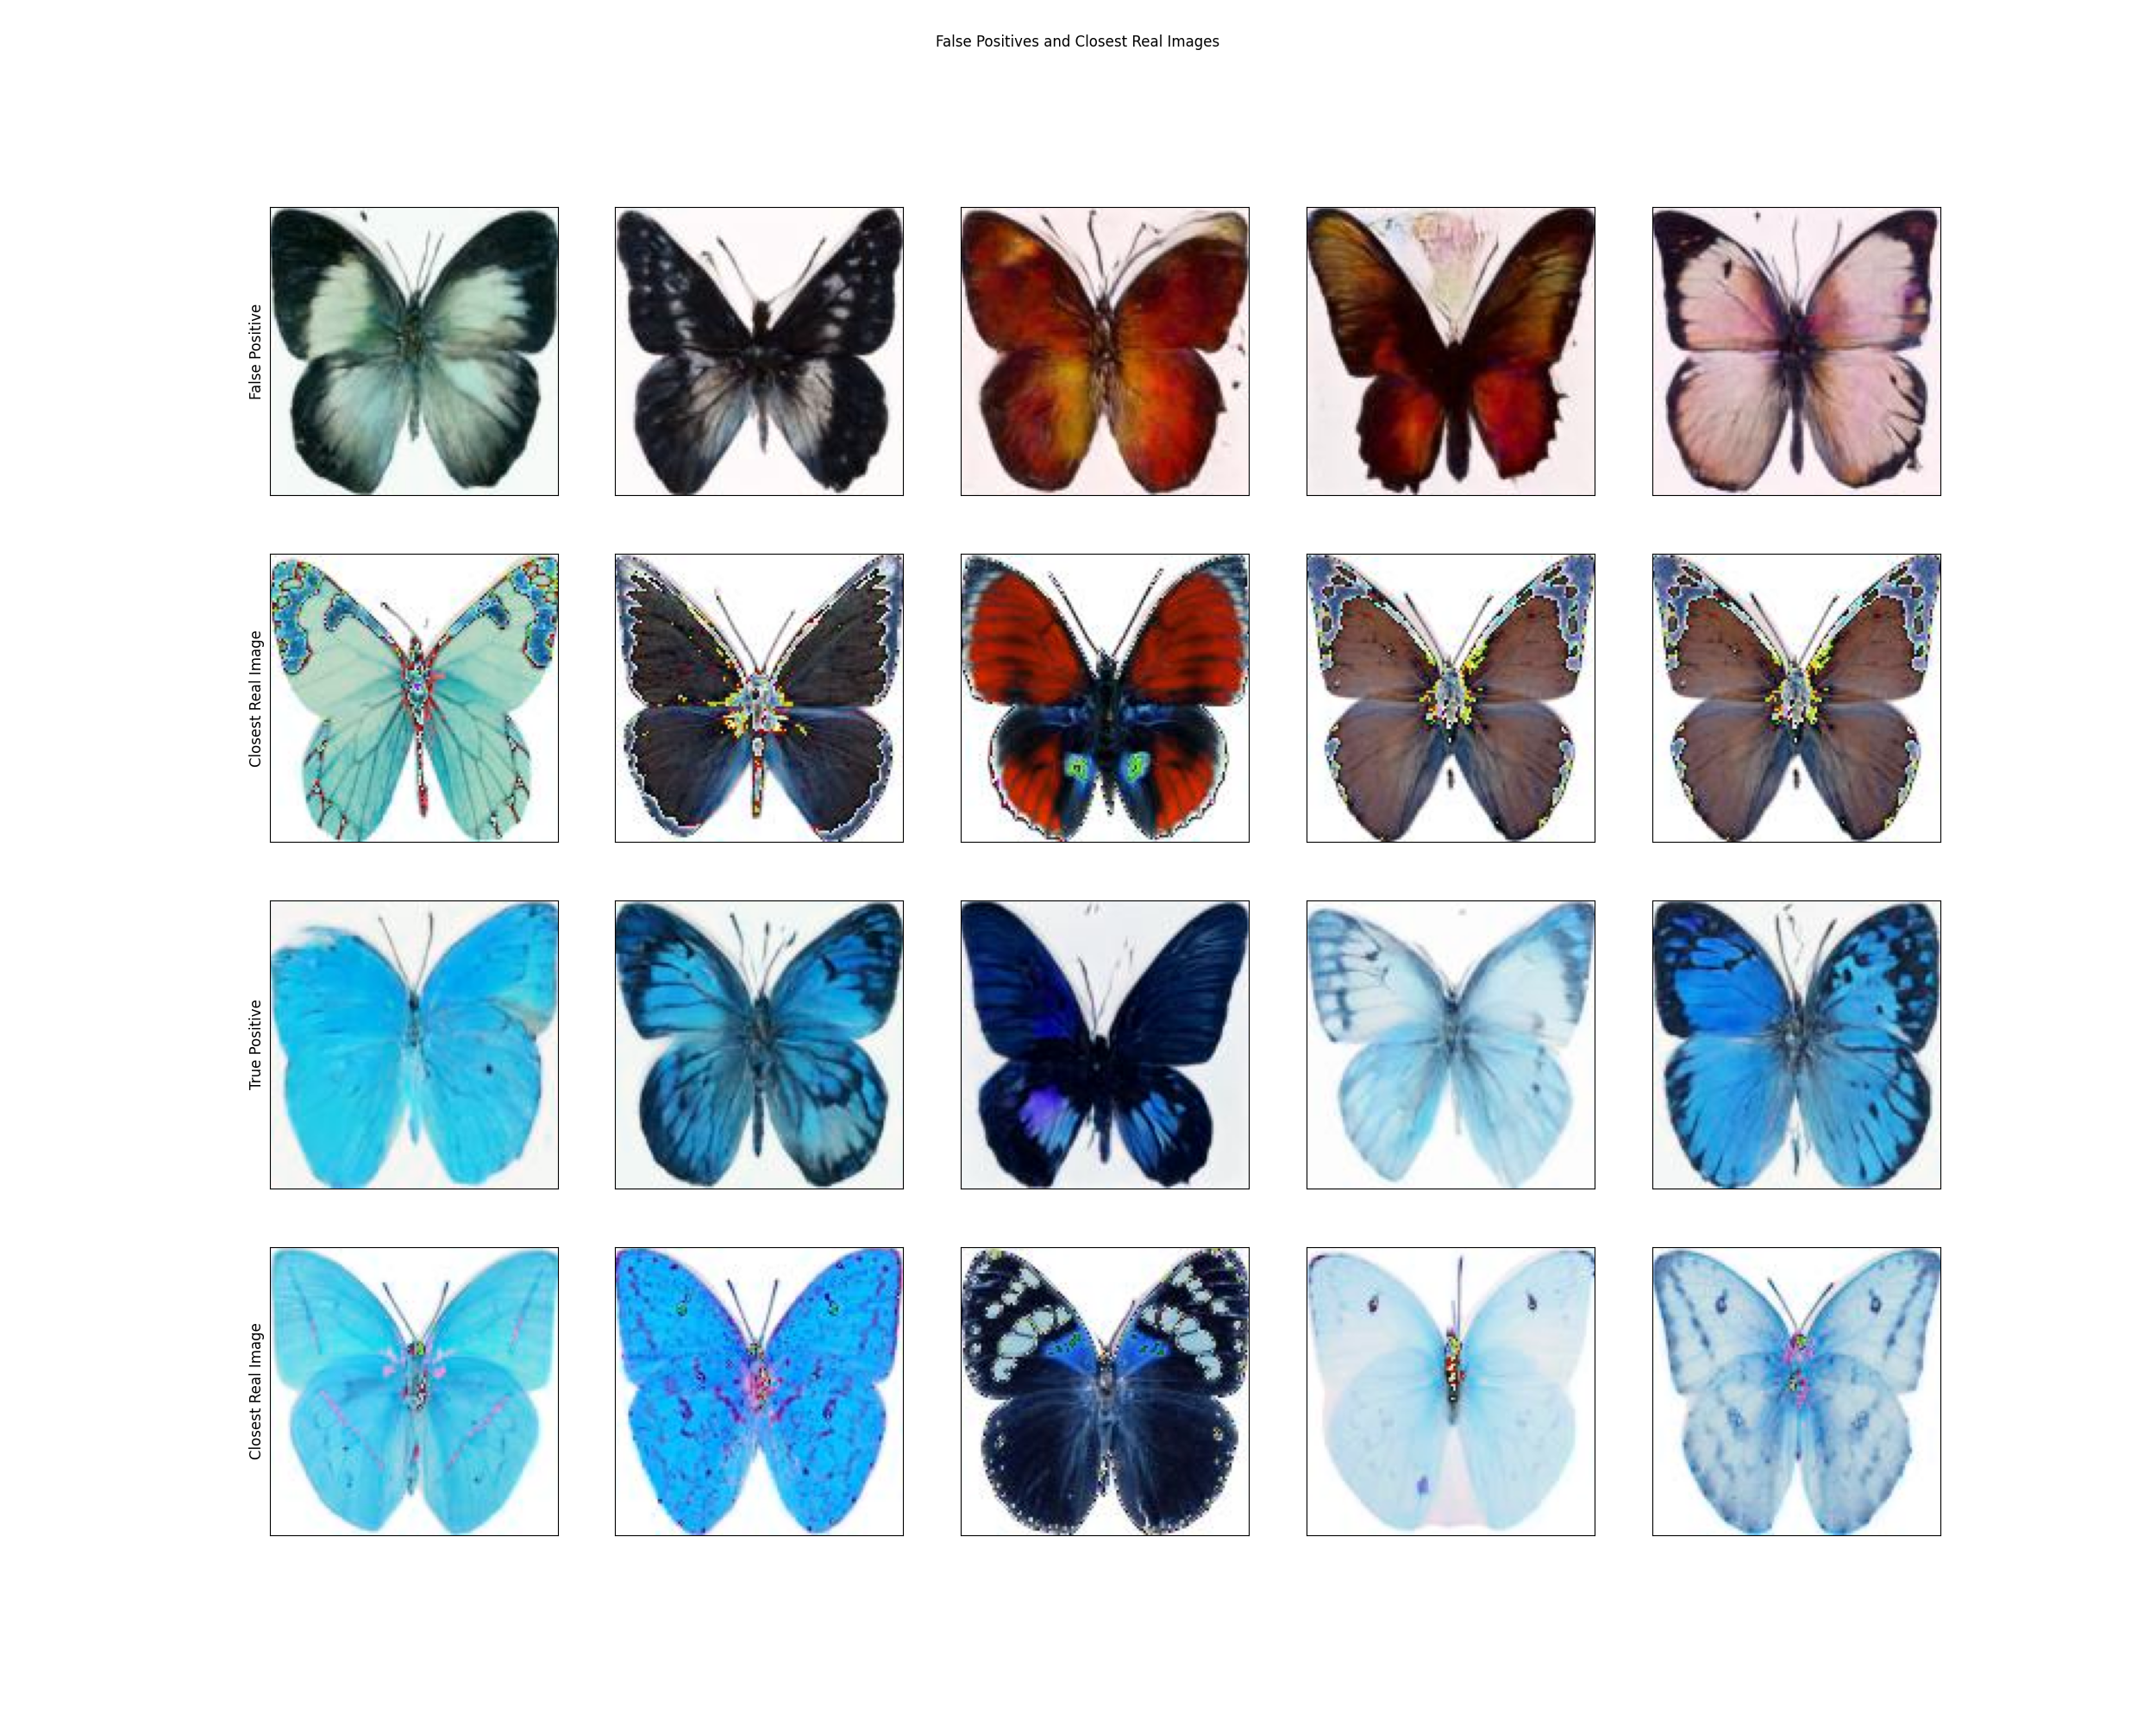
\includegraphics[width=0.45\textwidth]{../images/realworldexperiments/butterflies/examples/fp_hue_histogram.png}
    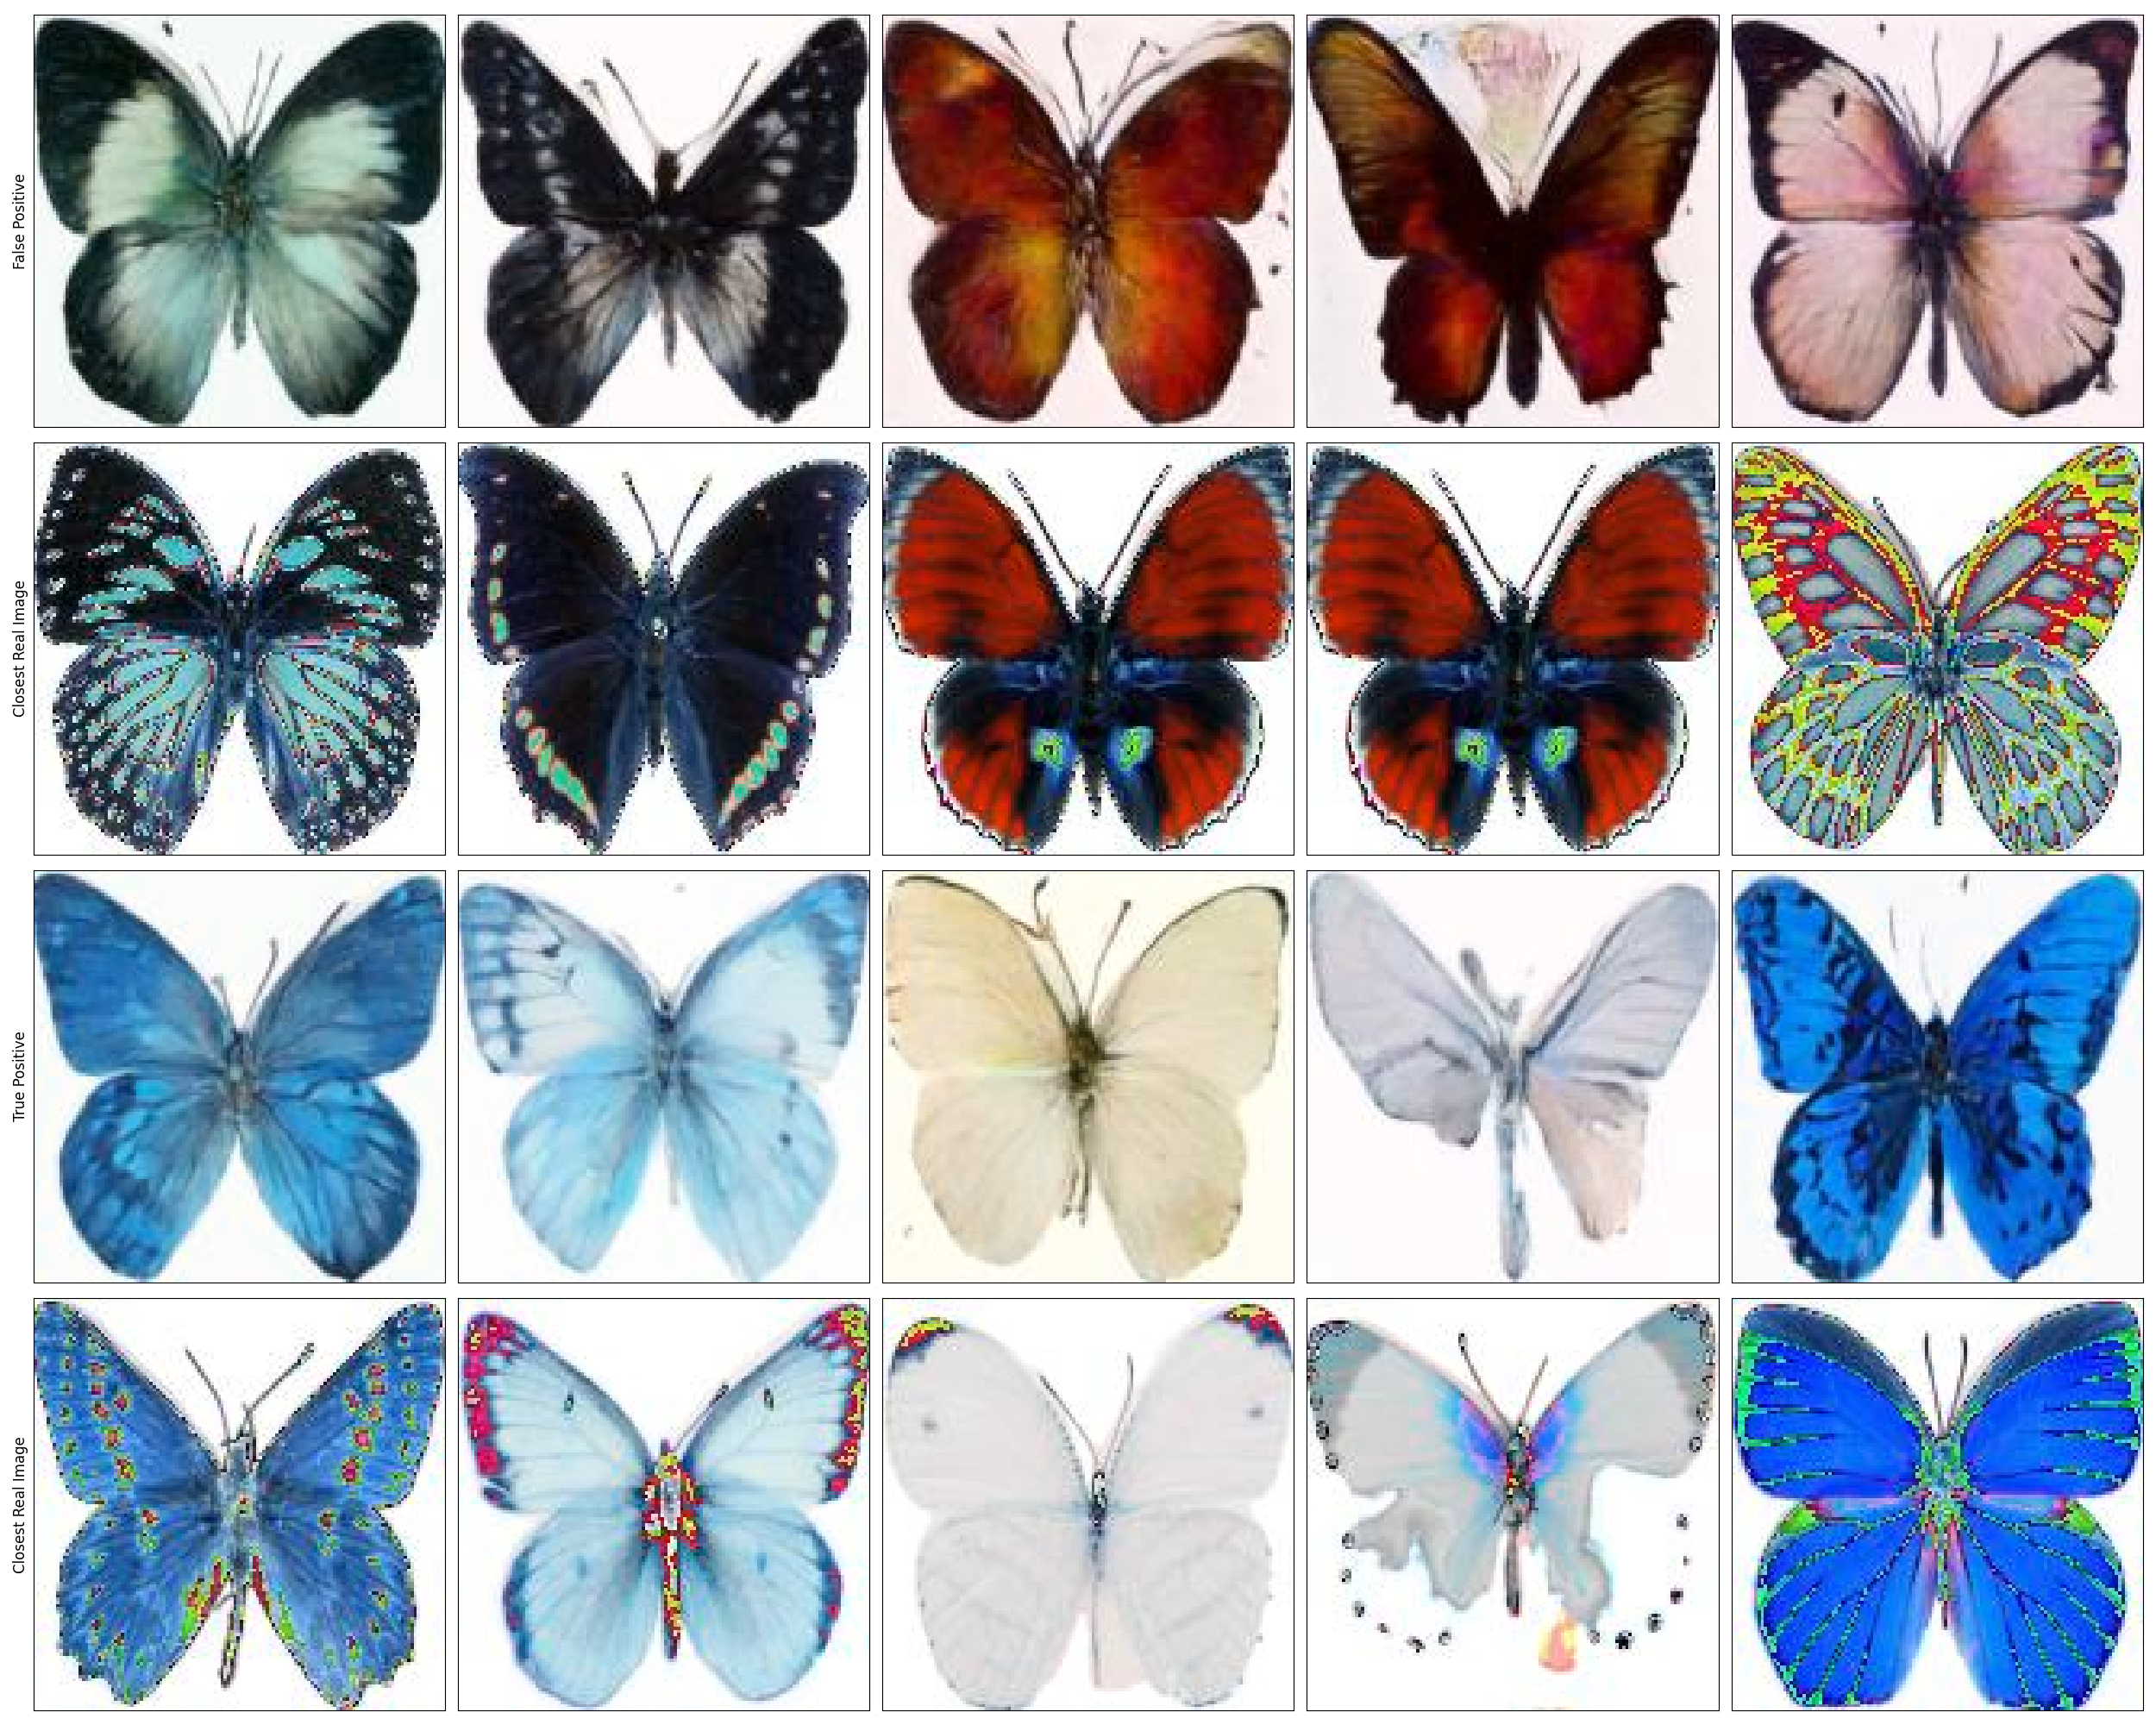
\includegraphics[width=0.45\textwidth]{../images/realworldexperiments/butterflies/examples/fp_rgb_histogram.png}
    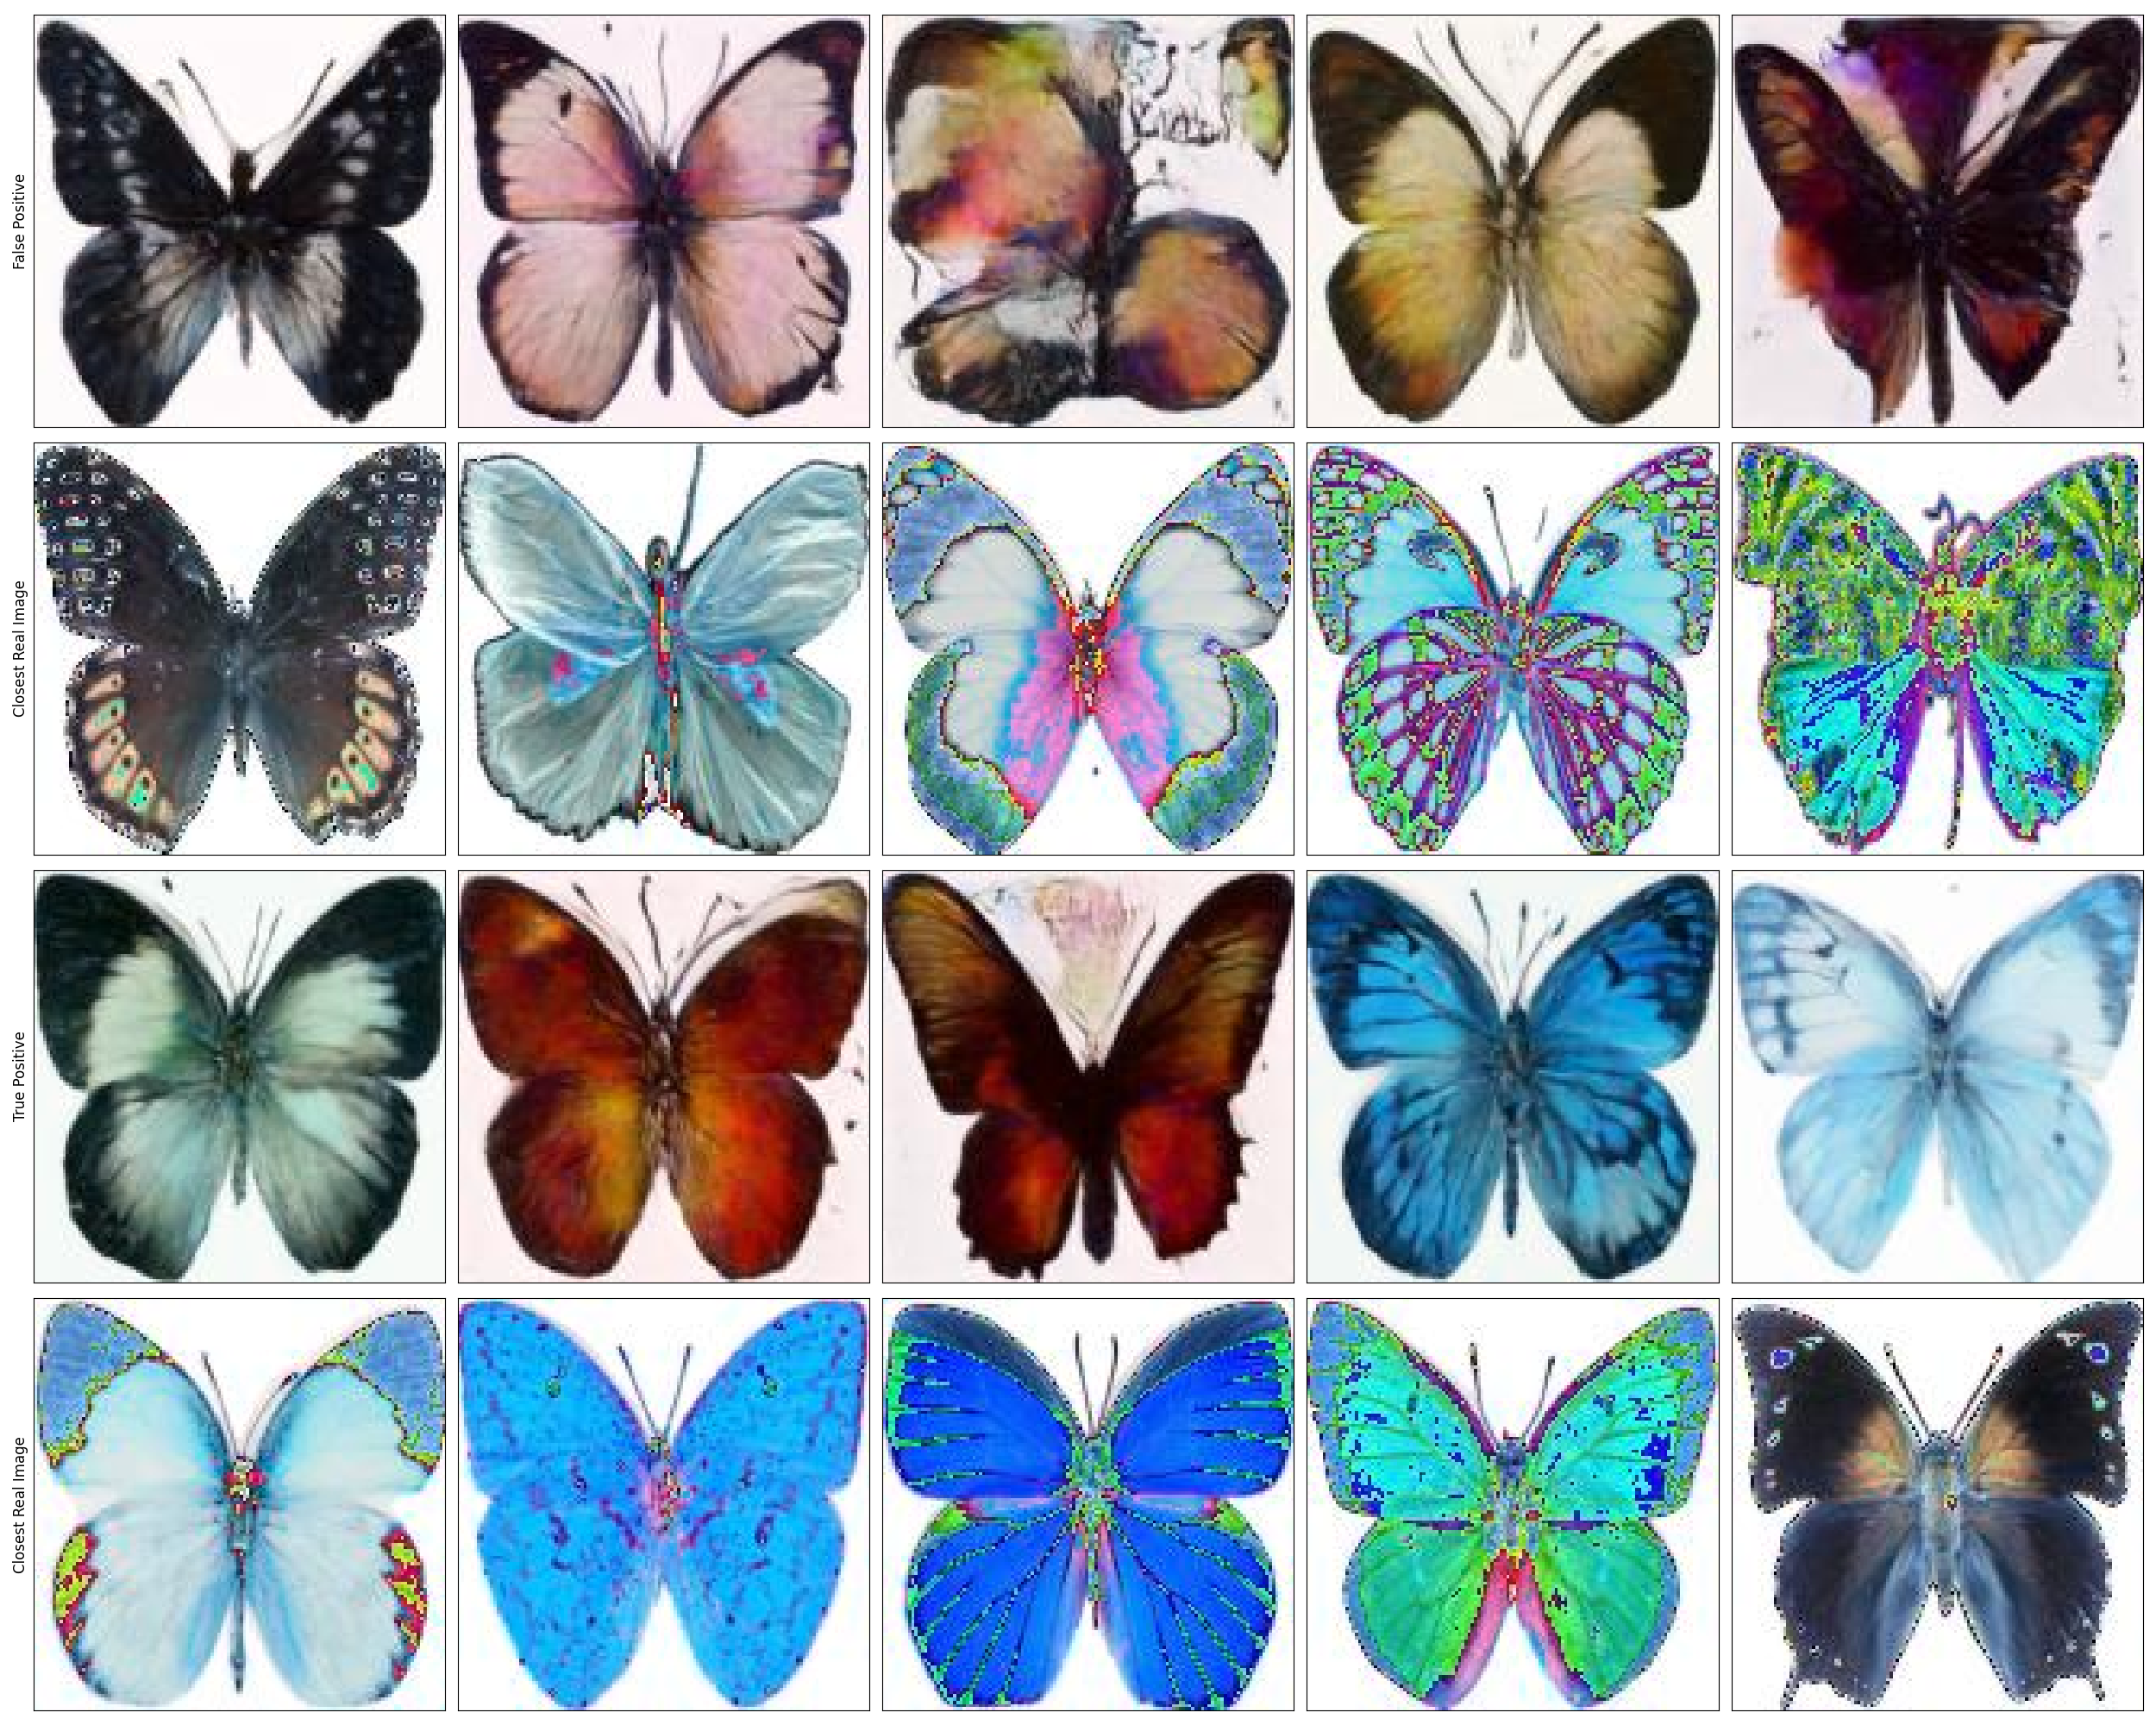
\includegraphics[width=0.45\textwidth]{../images/realworldexperiments/butterflies/examples/fp_saturation_histogram.png}
    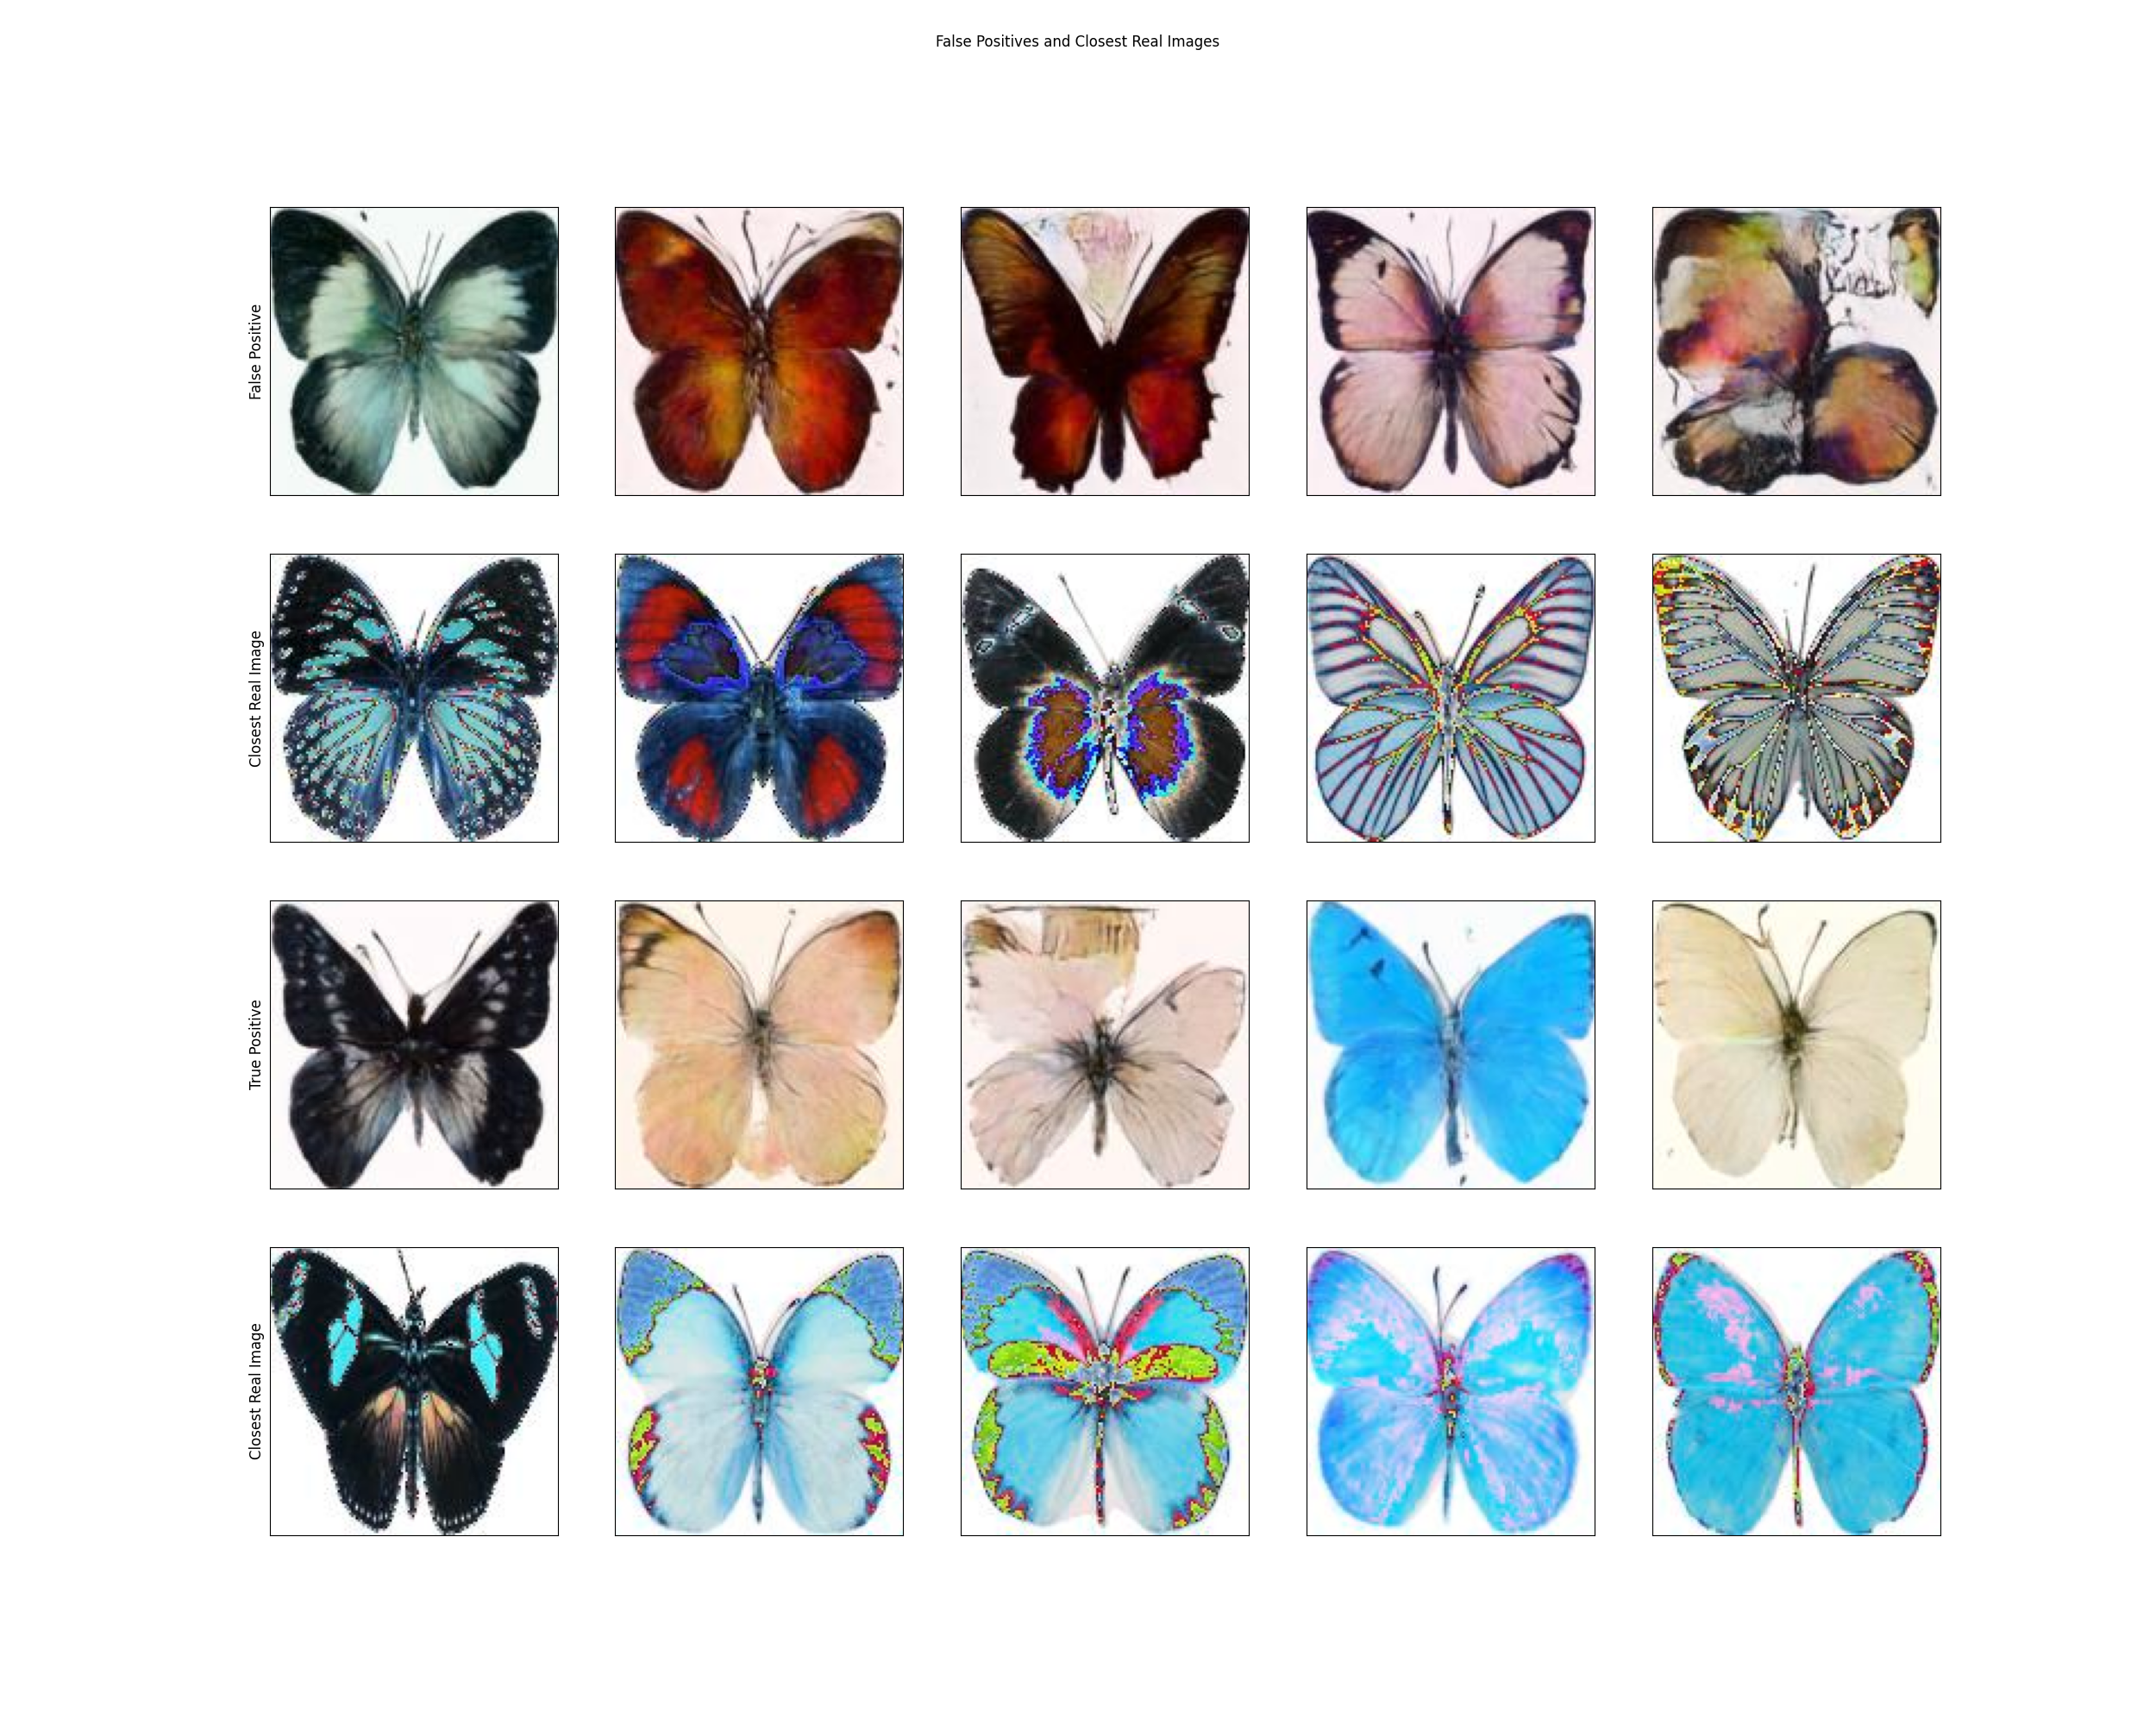
\includegraphics[width=0.45\textwidth]{../images/realworldexperiments/butterflies/examples/fp_value_histogram.png}
    \caption{l'ordine delle immagini da sinistra verso destra e dall'alto in basso è: grayscale, hsv, hue, rgb, saturation, value}
\end{figure}

La maggior parte dei falsi positivi e dei veri positivi sono risultati comuni a tutti gli istogrammi, indicando che questi catturano in modo coerente caratteristiche simili delle immagini.

I falsi positivi presentano frequentemente artefatti visivi o pattern innaturali, mentre i veri positivi, pur essendo più vicini alle immagini reali in termini di colore e luminosità, possono comunque mostrare aberrazioni. Questo è dovuto al fatto che gli istogrammi considerati non catturano informazioni spaziali, ma solo proprietà cromatiche. Le caratteristiche spaziali, fondamentali per identificare la struttura delle immagini, non vengono analizzate in questo approccio, limitando la capacità di distinguere campioni generati di alta qualità.

Ricordiamo inoltre che la selezione si è basata interamente su quei dati che ricadono o meno nel manifold definito dall'improved precision recall, che come visto dagli esperimenti sui toy dataset soffre della presenza di outliers. Dall'analisi della kde risulta che i dati reali sono meno sparsi rispetto ai dati generati, e quindi la presenza di outliers non dovrebbe essere particolarmente influente sull'identificazione dei falsi positivi. Dall'altra parte i dati generati sono più sparsi, è quindi probabile che ci sia una sovrastima del manifold di \(G\), portando a un elevato numero di falsi negativi e veri positivi reali.

I risultati quantitativi delle metriche sono riportati nella Tabella \ref{tab:metriche}. Questi dati evidenziano i compromessi tra precision, recall e altre metriche di performance.

\begin{table}[h!]
    \label{tab:metriche}
    \centering
    \resizebox{\textwidth}{!}{
    \begin{tabular}{lcccccccc}
        \hline
        \textbf{Istogramma} & \textbf{Precision} & \textbf{Recall} & \textbf{Density} & \textbf{Coverage} & \textbf{FPR*} & \textbf{FNR*} & \textbf{n. False Positives} & \textbf{n. True Positives} \\
        \hline
        Hue & 0.4654 & 0.9855 & 0.0720 & 0.1908 & 0.6897 & 0.0402 & 618 & 278 \\
        Saturation & 0.5904 & 0.9978 & 0.1833 & 0.7824 & 0.3996 & 0.0033 & 358 & 538 \\
        HSV & 0.3783 & 0.9866 & 0.0546 & 0.2254 & 0.6719 & 0.0112 & 602 & 294 \\
        RGB & 0.0446 & 0.9978 & 0.0120 & 0.1998 & 0.9096 & 0.0000 & 815 & 81 \\
        Value & 0.2578 & 0.9877 & 0.1113 & 0.7679 & 0.7366 & 0.0022 & 660 & 236 \\
        Grayscale & 0.1071 & 1.0000 & 0.0533 & 0.6763 & 0.9040 & 0.0000 & 810 & 86 \\
        \hline
    \end{tabular}
    }
    \caption{FPR* = False Positive Rate, FNR* = False Negative Rate}
\end{table}

Ai fini di utilizzare la metrica come filtro per i dati generati di alta qualità, siamo poco interessati alla statistica di recall tuttavia è apprezzabile che tutte le distanze considerate abbiano un valore di recall molto alto (che conferma le ipotesi sollevate dall'osservazione della kde).
La precision è molto variabile, con valori che vanno da 0.0446 a 0.5904. Sebbene la saturation registri il valore più alto, come si può vedere dagli esempi visivi, è probabile che la hue sia la metrica più adatta per identificare i falsi positivi.
Questi risultati confermano che, pur fornendo una base solida per l'analisi delle caratteristiche cromatiche, le metriche basate sugli istogrammi richiedono un'integrazione con descrittori spaziali per migliorare la capacità di discriminazione tra dati reali e generati di alta qualità.

\subsection{Scarlatti}

Come descritto nel capitolo precedente \ref{subsec:scarlatti}, i primi esperimenti condotti sul dataset degli Scarlatti sono finalizzati a verificare l'applicabilità della KDE per la rappresentazione delle distribuzione dei dati e a valutare la capacità descrittive delle caratteristiche scelte.
Per fare ciò sono riportati in seguito figura \ref{fig:realworldexperiments-scarlatti-real} i risultati delle KDE applicate alle distanze intra-set per i campioni reali divisi in training set e validation più test set.
Le distribuzioni risultano pressochè identiche, con una leggera differenza dovuta, con molta probabilità, alla diversa dimensione dei due set ( il trainig contiene 920 campioni, il validation 309 e il test 305).

\begin{figure}[!ht]
    \label{fig:realworldexperiments-scarlatti-real}
    \centering
    \includegraphics[width=0.3\textwidth]{../images/realworldexperiments/scarlatti/realdata/TrainVsTest_avgIOI.png}
    \includegraphics[width=0.3\textwidth]{../images/realworldexperiments/scarlatti/realdata/TrainVsTest_avgPitchShift.png}
    \includegraphics[width=0.3\textwidth]{../images/realworldexperiments/scarlatti/realdata/TrainVsTest_nNotesPerMeasure.png}
    \includegraphics[width=0.3\textwidth]{../images/realworldexperiments/scarlatti/realdata/TrainVsTest_noteLengthHist.png}
    \includegraphics[width=0.3\textwidth]{../images/realworldexperiments/scarlatti/realdata/TrainVsTest_noteLengthTransMatrix.png}
    \includegraphics[width=0.3\textwidth]{../images/realworldexperiments/scarlatti/realdata/TrainVsTest_nPitchesPerMeasure.png}
    \includegraphics[width=0.3\textwidth]{../images/realworldexperiments/scarlatti/realdata/TrainVsTest_pitchClassHist.png}
    \includegraphics[width=0.3\textwidth]{../images/realworldexperiments/scarlatti/realdata/TrainVsTest_pitchClassHistPerMeasure.png}
    \includegraphics[width=0.3\textwidth]{../images/realworldexperiments/scarlatti/realdata/TrainVsTest_pitchClassTransMatrix.png}
    \includegraphics[width=0.3\textwidth]{../images/realworldexperiments/scarlatti/realdata/TrainVsTest_pitchRange.png}
    \caption{l'ordine delle immagini da sinistra verso destra e dall'alto in basso è: avgIOI, avgPitchShift, nNotesPerMeasure, noteLengthHist, noteLengthTransMatrix, nPitchesPerMeasure, pitchClassHist, pitchClassHistPerMeasure, pitchClassTransMatrix, pitchRange}
\end{figure}

Possiamo notare che una delle caratteristiche, la \textbf{pitchRange}, presenta una distribuzione che, sebbene sia molto simile per i due set, fallisce l'approssimazione della bandwidth della KDE, portando alla presenza di picchi multipli. Questo è dovuto, oltre che alla scalarità della feature, alla sua discretezza.
I pitch range potendo assumere solo valori interi presenterà delle distanze intra-set intere a loro volta, e quindi la KDE non sarà in grado di approssimare correttamente la distribuzione. Gli esperimenti successivi riporteranno comunque i risultati per questa feature, ma è fondamentale ridimensionarne l'importanza.

Si passa ora alla valutazione delle metriche per i dati generati. I risultati ottenuti sono riportati in figura \ref{fig:realworldexperiments-scarlatti-fake}.

\begin{figure}[!ht]
    \centering
    \includegraphics[width=0.6\textwidth]{../images/realworldexperiments/scarlatti/violinplots/TrainVsFake_avgIOI.png}
    \includegraphics[width=0.3\textwidth]{../images/realworldexperiments/scarlatti/prcurves/PRCurveScarlatti_avgIOI.png}
\end{figure}
\begin{figure}[!ht]
    \centering
    \includegraphics[width=0.6\textwidth]{../images/realworldexperiments/scarlatti/violinplots/TrainVsFake_avgPitchShift.png}
    \includegraphics[width=0.3\textwidth]{../images/realworldexperiments/scarlatti/prcurves/PRCurveScarlatti_avgPitchShift.png}
\end{figure}  
\begin{figure}[!ht]
    \centering
    \includegraphics[width=0.6\textwidth]{../images/realworldexperiments/scarlatti/violinplots/TrainVsFake_nNotesPerMeasure.png}
    \includegraphics[width=0.3\textwidth]{../images/realworldexperiments/scarlatti/prcurves/PRCurveScarlatti_nNotesPerMeasure.png}
\end{figure} 
\begin{figure}[!ht]
    \centering
    \includegraphics[width=0.6\textwidth]{../images/realworldexperiments/scarlatti/violinplots/TrainVsFake_noteLengthHist.png}
    \includegraphics[width=0.3\textwidth]{../images/realworldexperiments/scarlatti/prcurves/PRCurveScarlatti_noteLengthHist.png}
\end{figure}   
\begin{figure}[!ht]
    \centering
    \includegraphics[width=0.6\textwidth]{../images/realworldexperiments/scarlatti/violinplots/TrainVsFake_noteLengthTransMatrix.png}
    \includegraphics[width=0.3\textwidth]{../images/realworldexperiments/scarlatti/prcurves/PRCurveScarlatti_noteLengthTransMatrix.png}
\end{figure}   
\begin{figure}[!ht]
    \centering
    \includegraphics[width=0.6\textwidth]{../images/realworldexperiments/scarlatti/violinplots/TrainVsFake_nPitchesPerMeasure.png}
    \includegraphics[width=0.3\textwidth]{../images/realworldexperiments/scarlatti/prcurves/PRCurveScarlatti_nPitchesPerMeasure.png}
\end{figure}  
\begin{figure}[!ht]
    \centering
    \includegraphics[width=0.6\textwidth]{../images/realworldexperiments/scarlatti/violinplots/TrainVsFake_pitchClassHist.png}
    \includegraphics[width=0.3\textwidth]{../images/realworldexperiments/scarlatti/prcurves/PRCurveScarlatti_pitchClassHist.png}
\end{figure}
\begin{figure}[!ht]
    \centering
    \includegraphics[width=0.6\textwidth]{../images/realworldexperiments/scarlatti/violinplots/TrainVsFake_pitchClassHistPerMeasure.png}
    \includegraphics[width=0.3\textwidth]{../images/realworldexperiments/scarlatti/prcurves/PRCurveScarlatti_pitchClassHistPerMeasure.png}
\end{figure}
\begin{figure}[!ht]
    \centering
    \includegraphics[width=0.6\textwidth]{../images/realworldexperiments/scarlatti/violinplots/TrainVsFake_pitchClassTransMatrix.png}
    \includegraphics[width=0.3\textwidth]{../images/realworldexperiments/scarlatti/prcurves/PRCurveScarlatti_pitchClassTransMatrix.png}
\end{figure}
\begin{figure}[!ht]
    \label{fig:realworldexperiments-scarlatti-fake}
    \centering
    \includegraphics[width=0.6\textwidth]{../images/realworldexperiments/scarlatti/violinplots/TrainVsFake_pitchRange.png}
    \includegraphics[width=0.3\textwidth]{../images/realworldexperiments/scarlatti/prcurves/PRCurveScarlatti_pitchRange.png}
    \caption{l'ordine delle immagini dall'alto in basso è: avgIOI, avgPitchShift, nNotesPerMeasure, noteLengthHist, noteLengthTransMatrix, nPitchesPerMeasure, pitchClassHist, pitchClassHistPerMeasure, pitchClassTransMatrix, pitchRange}
\end{figure}

Si può notare una generale tendenza delle pr-curves a confermare quanto osservato anche nelle kde. Come sollevato in ipotesi, per molte delle metriche si nota che con il passare delle epoche il modello generativo tende a generare dati sempre più simili a quelli reali, e quindi la sovrapposizione dei manifold di \(G\) e \(R\) aumenta.
In particolare il fenomeno è più evidente per le distanze matriciali quali \textbf{noteLengthTransMatrix} e \textbf{pitchClassTransMatrix}, e per il numero di altezze diverse per misura \textbf{nPitchesPerMeasure}. Meno marcato invece per le distanze scalari.
Un altro aspetto interessante è che, a meno delle \textbf{pitchClassHist} e \textbf{pitchClassTransMatrix} il modello generativo produce buoni risultati già alla seconda epoca di allenamento considerata, che risulta la migliore per numero di note per misura e per l'istogramma delle lunghezza delle note.
Questi risultati che vediamo nei grafici sono verificati anche numericamente, vedi tabella \ref{tab:res-scarlatti-supp}.

\begin{table}[h!]
    \textbf{Model - 011809}
    \centering
    \resizebox{\textwidth}{!}{
    \begin{tabular}{lccccccc}
        \hline
        \textbf{Feature} & \textbf{IP} & \textbf{IR} & \textbf{Density} & \textbf{Coverage} & \textbf{FPR} & \textbf{FNR} & \textbf{OA}\\ 
        \hline
        nNotesPM&0.6044&0.8956&0.3674&0.3911&0.3333&0.0822&0.7442 \\
        nPitchesPM&0.7211&0.9100&0.4904&0.5556&0.1922&0.0578&0.8335 \\
        pitchHist&0.8522&0.7978&0.7881&0.6611&0.2156&0.1811&0.7608 \\
        pitchHistPM&0.5489&0.6200&0.4296&0.5167&0.3811&0.3044&0.8639 \\
        pitchTrans&0.7311&0.2156&0.9330&0.5589&0.3578&0.6878&0.6215 \\
        pitchRange&0.0744&0.0267&0.0626&0.0122&0.0244&0.0144&0.9506 \\
        avgPitchShift&0.9189&0.9300&0.8807&0.7967&0.0189&0.0333&0.9477 \\
        avgIOI&0.4889&0.4322&0.3626&0.2833&0.1478&0.1000&\cellcolor{green}0.9178 \\
        lengthHist&0.7711&0.8800&0.7874&0.7522&0.2322&0.1056&0.8427 \\
        lengthHistPM&0.7811&0.8611&0.7511&0.7067&0.2411&0.1511&0.8656 \\
        lengthTrans&0.9489&0.7933&1.0593&0.6433&0.1656&0.2400&0.9043 \\
        \hline
    \end{tabular}
    }
\end{table}
\begin{table}[h!]
    \textbf{Model - 516209}
    \centering
    \label{tab:res-scarlatti-supp}
    \resizebox{\textwidth}{!}{
    \begin{tabular}{lccccccc}
        \hline
        \textbf{Feature} & \textbf{IP} & \textbf{IR} & \textbf{Density} & \textbf{Coverage} & \textbf{FPR} & \textbf{FNR} & \textbf{OA} \\ 
        \hline
        nNotesPM&0.7933&0.7900&0.6074&0.6278&\cellcolor{green}0.1533&0.1656&\cellcolor{green}0.8671 \\
        nPitchesPM&0.7978&0.7789&0.6793&0.6833&0.1178&0.1522&0.8758 \\
        pitchHist&0.9078&0.8511&1.0900&0.7956&0.0833&0.1800&0.9018 \\
        pitchHistPM&0.6222&0.6578&0.5841&0.6900&0.2733&0.2544&0.9118 \\
        pitchTrans&0.8978&0.3533&1.8900&0.8711&0.0911&0.6167&0.7370 \\
        pitchRange&0.0311&0.0222&0.0300&0.0144&0.0044&0.0122&\cellcolor{green}0.9809 \\
        avgPitchShift&0.9233&0.9067&0.8752&0.7867&0.0200&0.0489&0.9688 \\
        avgIOI&0.3778&0.3222&0.3078&0.2589&\cellcolor{green}0.0700&0.0933&0.8926 \\
        lengthHist&0.8600&0.8356&0.9978&0.8167&\cellcolor{green}0.1611&0.1656&\cellcolor{green}0.9335 \\
        lengthHistPM&0.8256&0.7967&0.8678&0.7778&\cellcolor{green}0.1122&0.2189&0.9497 \\
        lengthTrans&0.9722&0.8144&1.1374&0.7789&\cellcolor{green}0.0556&0.2500&0.9002 \\
        \hline
    \end{tabular}
    }
\end{table}
\begin{table}[h!]
    \textbf{Model - 2077006}
    \centering
    \resizebox{\textwidth}{!}{
    \begin{tabular}{lccccccc}
        \hline
        \textbf{Feature} & \textbf{IP} & \textbf{IR} & \textbf{Density} & \textbf{Coverage} & \textbf{FPR} & \textbf{FNR} & \textbf{OA} \\ 
        \hline
        nNotesPM&0.7533&0.8611&0.5519&0.5944&0.1878&0.1067&0.8549 \\
        nPitchesPM&0.7778&0.8300&0.6130&0.6467&0.1378&0.1311&0.9122 \\
        pitchHist&0.9111&0.8911&0.9100&0.8356&0.0856&0.0933&0.9111 \\
        pitchHistPM&0.6289&0.7733&0.5578&0.6622&0.2356&0.1589&0.9347 \\
        pitchTrans&0.8911&0.5789&1.2419&0.8778&0.1056&0.3711&0.9266 \\
        pitchRange&0.0289&0.0056&0.0241&0.0133&0.0022&0.0033&0.9283 \\
        avgPitchShift&0.9100&0.9222&0.8656&0.7844&0.0244&0.0422&0.9744 \\
        avgIOI&0.4467&0.4222&0.3533&0.2711&0.1278&0.0556&0.8827 \\
        lengthHist&0.7856&0.8933&0.7659&0.7478&0.2200&0.1100&0.8624 \\
        lengthHistPM&0.8156&0.8689&0.8567&0.7767&0.1611&0.1611&\cellcolor{green}0.9765 \\
        lengthTrans&0.9367&0.8811&1.0404&0.8333&0.1011&0.1733&0.9595 \\
        \hline
    \end{tabular}
    }
\end{table}
\begin{table}[h!]
    \textbf{Model - 7083228}
    \centering
    \resizebox{\textwidth}{!}{
    \begin{tabular}{lccccccc}
        \hline
        \textbf{Feature} & \textbf{IP} & \textbf{IR} & \textbf{Density} & \textbf{Coverage} & \textbf{FPR} & \textbf{FNR} & \textbf{OA} \\ 
        \hline
        nNotesPM&0.7767&0.8456&0.5937&0.6167&0.1767&0.1211&0.8615 \\
        nPitchesPM&0.8156&0.8333&0.6463&0.6867&\cellcolor{green}0.1067&0.1033&\cellcolor{green}0.9518 \\
        pitchHist&0.9200&0.9111&0.9515&0.8689&0.0789&0.1056&0.9458 \\
        pitchHistPM&0.7322&0.7722&0.6519&0.7556&0.1656&0.1744&0.9305 \\
        pitchTrans&0.8911&0.7122&1.1104&0.9089&\cellcolor{green}0.0856&0.2589&\cellcolor{green}0.9719 \\
        pitchRange&0.0478&0.0056&0.0426&0.0167&\cellcolor{green}0.0000&0.0022&0.9704 \\
        avgPitchShift&0.9156&0.9000&0.8641&0.8067&0.0267&0.0356&0.9474 \\
        avgIOI&0.4633&0.4656&0.3493&0.2622&0.1344&0.0589&0.9006 \\
        lengthHist&0.7978&0.9100&0.7593&0.8067&0.1778&0.0978&0.8585 \\
        lengthHistPM&0.8378&0.8811&0.8859&0.8233&0.1344&0.1322&0.9657 \\
        lengthTrans&0.9267&0.8978&0.9889&0.8311&0.1111&0.1244&0.9693 \\
        \hline
    \end{tabular}
    }
\end{table}
\begin{table}[h!]
    \textbf{Model - 7969400}
    \centering
    \resizebox{\textwidth}{!}{
    \begin{tabular}{lccccccc}
        \hline
        \textbf{Feature} & \textbf{IP} & \textbf{IR} & \textbf{Density} & \textbf{Coverage} & \textbf{FPR} & \textbf{FNR} & \textbf{OA} \\ 
        \hline
        nNotesPM&0.7922&0.8289&0.6074&0.6167&0.1567&0.1289&0.8574 \\
        nPitchesPM&0.8156&0.8578&0.6822&0.7367&0.1133&0.0922&0.9425 \\
        pitchHist&0.9256&0.8967&0.9215&0.8667&\cellcolor{green}0.0722&0.1167&\cellcolor{green}0.9548 \\
        pitchHistPM&0.7456&0.7656&0.6800&0.7767&\cellcolor{green}0.1489&0.1767&\cellcolor{green}0.9491 \\
        pitchTrans&0.8922&0.7000&1.0985&0.9011&0.1133&0.2567&0.9700 \\
        pitchRange&0.0389&0.0056&0.0348&0.0167&0.0033&0.0000&0.9504 \\
        avgPitchShift&0.9322&0.9256&0.8930&0.8144&\cellcolor{green}0.0156&0.0400&\cellcolor{green}0.9897 \\
        avgIOI&0.4367&0.4322&0.3478&0.2656&0.1144&0.0478&0.8864 \\
        lengthHist&0.8111&0.8933&0.7648&0.7744&0.1789&0.1033&0.8685 \\
        lengthHistPM&0.8489&0.8644&0.8870&0.8178&0.1144&0.1589&0.9499 \\
        lengthTrans&0.9378&0.8956&1.0115&0.8656&0.1033&0.1433&\cellcolor{green}0.9614 \\
        \hline
    \end{tabular}
    }
    \caption{I risultati ottenuti con l'identificazione dei falsi positivi tramite supporto (indicata con OA l'Overlapped Area)}
\end{table}

Quello che si nota e che giustifica gli esperimenti successivi è che non sempre c'è una corrispondenza fra il modello con minor numero di falsi positivi e maggior overlapped area. Questo vale in particolare proprio per il modello appena citato, il 516209, che presenta spesso il maggior numero di falsi positivi ma anche il maggior numero di falsi negativi. 
Se si osserva i valori della density e della coverage possiamo facilmente stabilire che questa epoca tende a generare dati con poca varianza, \textit{diversity}. Vogliamo quindi verificare se si ottengono gli stessi risultati operando invece che con il supporto dell'improved precision-recall, con le kde.
Utilizzare un diverso approccio permette, oltre che mezzo di confronto, controprova per la validità dei risultati ottenuti. 

Come indicato nel capitolo precedente \ref{subsec:scarlatti}, utilizzando un percentile fisso per la selezione dei falsi positivi, si ottiene sempre lo stesso numero di outliers indipendentemente dal modello. Tuttavia si può verificare sperimentalmente che i risultati prodotti sono migliori rispetto a quelli ottenuti con il supporto dell'improved precision-recall. 
Un ascolto degli esempi raccolti con questo metodo verifica immediatamente che i falsi positivi sono effettivamente dati generati di bassa qualità, sono infatti discriminati quei dati mal generati che non hanno il numero corretto di misure, sono individuati i dati che tendono a ripetere sempre la stessa nota e lo stesso vale per i dati che presentano pause o passaggi armonici poco naturali.

\chapter{Note Implementative}\label{ch:notes}

Per la generazione di dataset con distribuzione uniforme è stata utilizzata la funzione \texttt{numpy.random.uniform}, mentre per la generazione di dataset con distribuzione normale è stata utilizzata la funzione \texttt{numpy.random.multivariate\_normal} di numpy. La prima oltre alla dimensione dei sample e al numero prende come parametri anche il range di valori che i dati possono assumere, mentre la seconda prende come parametri lo shift (che di default è 0). Come media avremo quindi \texttt{shift*numpy.ones(dim)} e come covarianza la matrice identità (\texttt{numpy.eye(dim)}).\
Sono state poi adottate una serie di funzioni per facilitare il debugging attraverso la visualizzazione dei dati. In particolare una funzione che mostri dati di due dimensioni con il corrispondente manifold e fuzioni come il \textbf{realism score} che permette di valutare la verosimiglianza dei singoli dati generati.\

Questi grafici sono stati prodotti utilizzando la libreria \texttt{matplotlib} di python.

\addcontentsline{toc}{chapter}{Bibliografia}
\bibliographystyle{plain}
\bibliography{files/biblio}
\bibliographystyle{unsrt}
%\bibliography{sp,xml}

\end{document} 
